\chapter*{Chapter 152: \\
	Zoning}
    \addstarredchapter{Chapter 152: Zoning}
    \minitoc
    \pagebreak

\subchapter{GENERAL PROVISIONS}

\section{Intent and Purpose\footnote{(‘83 Code, SEC. 11.01)}}
This chapter is adopted for the purpose of:
\begin{enumerate}[{\indent}A)]
    \item Protecting the public health, safety, comfort, convenience and general welfare; 
    \item Promoting orderly development of the residential, commercial, industrial, recreational and public areas; 
    \item Conserving the natural and scenic beauty and attractiveness of the city; 
    \item Conserving and developing natural resources in the city; 
    \item Providing for the compatibility of different land uses and the most appropriate use of land throughout the city; 
    \item Minimizing environmental pollution; and
    \item Conserving energy through the use of solar systems and the encouragement of solar and earth-sheltered structures for commercial, industrial, and residential uses.
\end{enumerate}
\section{Rules of Language Construction}
Whenever a word or term defined hereinafter appears in the text of this chapter, its meaning shall be construed as set forth in the definition. All measured distances expressed in feet shall be to the nearest tenth of a foot.\footnote{(‘83 Code, SEC. 11.02)}
\section{Definitions\footnote{(‘83 Code, SEC. 11.03)}}
For the purpose of this chapter the following definitions shall apply, unless the context clearly indicates or requires a different meaning.
\begin{description}
    \item[ACCESSORY USE OR STRUCTURE] A use or structure on the same lot with, and of a nature customarily incidental and subordinate to, the principal use or structure. \footnote{(Ord. 86, 2nd Series, effective 12-23-93)}
    \item[ADULT ARCADE] An establishment where, for any form of consideration, one or more motion picture projectors, slide projectors, or similar machines for viewing by five (5) or fewer persons each are used to show films, motion pictures, video cassettes, slides, or other photographic reproductions that are characterized by an emphasis upon the depiction or description of specified sexual activities or specified anatomical areas.
    \item[ADULT BOOKSTORE] An establishment that has as a substantial portion of its stock—in—trade and offers for sale, for any form of consideration, any one or more of the following: 1) books, magazines, periodicals, or other printed matter, or photographs, films, motion pictures, video cassettes, slides, or other visual representation that are characterized by an emphasis upon the depiction or description of specified sexual activities or specified anatomical areas; or 2) instruments, devices, or paraphernalia that are designed for use in connection with specified sexual activities.
    \item[ADULT CABARET] A nightclub, bar, restaurant, or similar establishment that regularly features live performances that are characterized by the exposure of specified anatomical areas or by specified sexual activities, or films, motion pictures, video cassettes, slides, or other photographic reproductions in which a substantial portion of the total presentation time is devoted to the showing of material that is characterized by an emphasis upon the depiction or description of specified sexual activities or specified anatomical areas.
    \item[ADULT MOTION PICTURE THEATER] An establishment where, for any form of consideration, films, motion pictures, video cassettes, slides, or similar photographic reproductions are shown, and in which a substantial portion of the total presentation time is devoted to the showing of material characterized by an emphasis on the depiction or description of specified sexual activities or specified anatomical areas.
    \item[ADULT THEATER] A theater, concert hall, auditorium, or similar establishment characterized by (activities featuring) the exposure of specified anatomical areas or by specified sexual activities.
    \item[ADULT USE ESTABLISHMENTS] Adult use establishments include, but are not limited to: adult arcade, adult bookstore, adult cabaret, adult motion picture theater, adult theater, or sexual encounter establishment.
    \item[AGRICULTURAL BUILDING OR STRUCTURE] Any building or structure existing or erected which is used principally for agricultural purposes, with the exception of dwelling units.
    \item[AGRICULTURAL USE] The use of land for the growing and/or production of field crops, livestock, and livestock products for the production of income, including but not limited to the following:
        \begin{enumerate}[{\indent\indent}1)]
            \item Field crops, including barley, soy beans, corn, hay, oats, potatoes, rye, sorghum, and sunflowers.
            \item Livestock, including dairy and beef cattle, goats, horses, sheep, hogs, poultry, game birds and other animals including dogs, ponies, deer, rabbits and mink.
            \item Livestock products, including milk, butter, cheese, eggs, meat, fur and honey.
        \end{enumerate}
    \item[APARTMENT] A room or suite of rooms with cooking facilities available which is occupied as a residence by a single family, or a group of individuals living together as a single family unit.  This includes any unit in buildings with more than two dwelling units.
    \item[APARTMENT BUILDING, HIGH RISE] An apartment building three or more stories in height, whose upper floors are accessible by elevator, and whose dwelling units are accessible through common corridors.
    \item[APARTMENT BUILDING, WALKUP] An apartment building not more than three stories above grade whose upper floors are accessible by stairs, and whose dwelling units are usually accessible through common corridors.
    \item[AUTO OR MOTOR VEHICLE REDUCTION YARD] A lot or yard where one or more unlicensed motor vehicle(s), or the remains thereof, are kept for the purpose of dismantling, wrecking, crushing, repairing, rebuilding, sale of parts, sale as scrap, storage, or abandonment. (See also JUNK YARD).
    \item[AUTOMOBILE SERVICE STATION] A building designed primarily for the supplying of motor fuel, oil, lubrication and accessories to motor vehicles or any portion thereof. \footnote{(Ord. 537, effective 7-1-83)}
    \item[BASEMENT] Any area of a structure, including crawl space, having its floor or base subgrade (below ground level) on all four sides, regardless of the depth of excavation below ground level. \footnote{(Ord. 86, 2nd Series, effective 12-23-93)}
    \item[BED AND BREAKFAST INN] An owner occupied building at least 75 years old designed for and used as a single-family or two-family dwelling that provides four or fewer lodging rooms accommodating no more than eight adults, in which meals are provided to overnight guests, and that is open to the traveling public for a stay not to exceed 20 days. \footnote{(Ord. 37, 2nd Series, effective 9-16-86)}
    \item[BOARDING HOUSE (ROOMING OR LODGING HOUSE)] A building other than a motel or hotel where, for compensation and by prearrangement for definite periods, meals or lodging are provided for three or more persons, but not to exceed 20 persons.
    \item[BUILDING] Any structure having a roof which may provide shelter or enclosure of persons, animals, chattel, or property of any kind and when the structures are divided by party walls without openings, each portion of the building so separated shall be deemed a separate building.
    \item[BUILDING LINE] A line parallel to the street right-of-way line at any story level of a building and representing the minimum distance which all or any part of the building is set back from the right-of-way.
    \item[BUILDING HEIGHT] The vertical distance to be measured from the average grade of a building line to the top, to the cornice of a flat roof, to the deck line of a mansard roof, to a point on the roof directly above the highest wall of a shed roof, to the uppermost point on a round or other arch type roof, to the mean distance of the highest gable on a pitched or hip roof.
    \item[BUILDING SETBACK] The minimum horizontal distance between the building and a lot line, or the normal high water mark of a stream or river.
    \item[BUSINESS] Any occupation, employment or enterprise wherein merchandise is exhibited or sold, or where services are offered for compensation.
    \item[CARPORT] An automobile shelter having two or more sides open. Floor of carport shall be of approved non-combustible material.
    \item[CELLAR] That portion of a building having more than one-half of the floor-to-ceiling height below the average grade of the adjoining ground.
    \item[CHURCH]  A building, together with its accessory buildings and uses, where persons regularly assemble for religious worship and which building, together with its accessory buildings and uses, is maintained and controlled by a religious body organized to sustain public worship.
    \item[CLEAR-CUTTING] The removal of an entire stand of vegetation.
    \item[CLUSTERING/CLUSTER HOUSING] The development pattern and technique whereby structures are arranged in closely related groups to make the most efficient use of the natural amenities of the land.
    \item[COMMISSIONER] Commissioner of the Department of Natural Resources. \footnote{(Ord. 537, effective 7-1-83)}
    \item[COMPREHENSIVE PLAN] A compilation of goals, policy statements, standards, programs and maps for guiding the physical, social and economic development, both public and private, of the city and its environs, as defined in the Municipal Planning Act, and includes any unit or part of the plan separately adopted and any amendment to the plan or parts thereof.
    \item[CONDITIONAL USE] A specific type of structure or land use that may be allowed but only after an in-depth review procedure and with appropriate conditions or restrictions as provided in the official zoning controls or building codes and upon a finding that\footnote{(Ord. 86, 2nd Series, effective 12-23-93)}:
        \begin{enumerate}[{\indent\indent}1)]
            \item Certain conditions as detailed in the zoning regulations exist; and 
            \item The structure and/or land use conform to the comprehensive land use plan (if one exists) and are compatible with the existing neighborhood.
        \end{enumerate}
    \item[CONDOMINIUM] A form of individual ownership of a multi-family building with joint responsibility for maintenance and repairs of the common property.  In a condominium, each apartment or townhouse unit is owned outright by its occupant and each occupant also owns a share of the land and other common property of the building.
    \item[COOPERATIVE] A multi-unit development operated for and owned by its occupants.  Individual occupants do not own their specific housing unit outright as in a condominium, but they own shares in the total enterprise.
    \item[CURB LEVEL] The grade elevation established by the Council of the curb in front of the center of the building.  Where no curb level has been established, the engineering staff shall determine a curb level or its equivalent for the purpose of this chapter.
    \item[DRIVE-IN] Any use where products and/or services are provided to the customer under conditions where the customer does not have to leave the car or where service to the automobile occupants is offered regardless of whether service is also provided within a building.
    \item[DWELLING UNIT] A residential building or portion thereof intended for occupancy by a single family but not including hotels, motels, boarding or rooming houses or tourist homes.  There are three principal types:
        \begin{enumerate}[{\indent\indent}1)]
            \item \textbf{MULTIPLE-FAMILY} A residence designed for or occupied by three or more families, either wholly (attached) or partially a part of a larger structure (detached), with separate housekeeping and cooking facilities for each.
            \item \textbf{SINGLE-FAMILY} A free-standing (detached) residence structure designed for or occupied by one family only.
            \item \textbf{TWO-FAMILY} A residence designed for or occupied by two families only, with separate housekeeping and cooking facilities for each.
        \end{enumerate}
    \item[DWELLING, ATTACHED] One which is joined to another dwelling or building at one or more sides by a party wall or walls.
    \item[DWELLING, DETACHED] One which is entirely surrounded by open space on the same lot.
    \item[EARTH SHELTERED BERM] An earth covering on the above grade portions of building walls.
    \item[EARTH SHELTERED BUILDING] A building constructed so that 50\% or more of the completed structure is covered with earth.  Earth covering is measured from the lowest level of livable space in residential units and of usable space in non-residential buildings.  An earth sheltered building is a complete structure that does not serve just as a foundation or substructure for aboveground construction.  A partially completed building shall not be considered earth sheltered.
    \item[EASEMENT] A grant by a property owner for the use of a strip of land for the purpose of constructing and maintaining walkways; roadways; utilities, including but not limited to sanitary sewers, water mains, electric lines, telephone lines, storm sewer or storm drainageways and gas lines.
    \item[EFFICIENCY UNIT] A dwelling unit with one primary room which doubles as a living room, kitchen and bedroom. \footnote{(Ord. 537, effective 7-1-83)}
    \item[EQUAL DEGREE OF ENCROACHMENT] A method of determining the location of floodway boundaries so that flood plain lands on both sides of a stream are capable of conveying a proportionate share of flood flows. \footnote{(Ord. 86, 2nd Series, effective 12-23-93)}
    \item[ESSENTIAL SERVICES] Overhead or underground electrical, gas, steam or water transmission or distribution systems and structures or collection, communication, supply or disposal systems and structures used by public utilities or governmental departments or commissions or as are required for the protection of the public health, safety or general welfare, including towers, poles, wires, mains, drains, sewers, pipes, conduits, cables, fire alarm boxes, police call boxes and accessories in connection herewith but not including buildings.  For the purpose of this chapter, the word “buildings” does not include “structures” for essential services.
    \item[EXTERIOR STORAGE (INCLUDES OPEN STORAGE)] The storage of goods, materials, equipment, manufactured products and similar items not fully enclosed by a building.
    \item[EXTRACTION AREA] Any non-agricultural artificial excavation of earth exceeding 50 square feet of surface area of two feet in depth, other than activity involved in preparing land for earth sheltered or conventional construction of residential, commercial, and industrial buildings, excavated or made by the removal from the natural surface of the earth, of sod, soil, sand, gravel, stone or other natural matter, or made by turning, or breaking or undermining the surface of the earth, except that public improvement projects shall not be considered \textbf{EXTRACTION AREAS}.
    \item[FAMILY] An individual, or two or more persons related by blood, marriage or adoption, living together as a single housekeeping unit in a dwelling unit.
    \item[FARM] A tract of land which is principally used for agricultural activities such as the production of cash crops, livestock or poultry farming.  The farms may include agricultural dwelling and accessory buildings and structures necessary to the operation of the farm.
    \item[FEEDLOTS, LIVESTOCK] The place of confined feeding of livestock, poultry or other animals for food, fur, pleasure or resale purposes in yards, lots, pens, buildings, or other areas not normally used for pasture or crops and in which substantial amounts of manure or related other wastes may originate by reason of the feeding of animals.
    \item[FENCE] Any partition, structure, wall or gate erected as a divider marker, barrier or enclosure and located along the boundary, or within the required yard. \footnote{(Ord. 537, effective 7-1-83)}
    \item[FLOOD] A temporary increase in the flow or stage of a stream or in the stage of a wetland or lake that results in inundation of normally dry areas.
    \item[FLOOD FREQUENCY] The frequency for which it is expected that a specific flood stage or discharge may be equaled or exceeded.
    \item[FLOOD FRINGE] That portion of the flood plain outside of the floodway. Flood fringe is synonymous with the term "floodway fringe" used in the Flood Insurance Study and Letter of Map Revision for the City of Crookston and is comprised of those areas designated “Zone AE" for the Red Lake River that are outside of the designated floodway on the Flood Insurance Rate Map and those “Zone AE” areas designated for the North and South Ponding Areas on the Flood Insurance Rate Map.
    \item[FLOOD PLAIN] The beds proper and the areas adjoining a wetland, lake or watercourse which have been or hereafter may be covered by the regional flood. \footnote{(Ord. 86, 2nd Series, effective 12-23-93)}
    \item[FLOOD PROOFING] A combination of structural provisions, changes or adjustments to properties and structures subject to flooding, primarily for the reduction or elimination of flood damages. \footnote{(Ord. 537, effective 7-1-83)}
    \item[FLOODWAY] The bed of a wetland or lake and the channel of a watercourse and those portions of the adjoining flood plain which are reasonably required to carry or store the regional flood discharge. \footnote{(Ord. 86, 2nd Series, effective 12-23-93)}
    \item[FLOOR AREA] The gross area of the main floor of a residential building measured in square feet and not an attached garage, breezeway or similar attachment.
    \item[FLOOR AREA, GROSS]The sum of the gross area of the various floors of a building measured in square feet. The basement floor area shall not be included unless the area constitutes a story.
    \item[FLOOR AREA RATIO] The numerical value obtained through dividing the gross floor area of a building or buildings by the net area of the lot or parcel of land on which the building or buildings are located.
    \item[FORESTRY] The use and management including logging of a forest, woodland or plantation and related research and educational activities, including the construction, alteration or maintenance of woodroads, skidways, landings, and fences.
    \item[FRONTAGE] That boundary of a lot which abuts an existing or dedicated public street.
    \item[GARAGE, PRIVATE] An accessory building or accessory portion of the principal building which is intended for and used to store the private passenger vehicles of the family or families resident upon the premises.
    \item[GRADE] The average of the finished level at the center of the exterior walls of the building.  For an earth sheltered building GRADE means the average of the finished level at the center of the lot.  For a building with earth berms but less than 50\% earth covering grade means the average of the finished level at the center of the building at the beginning of the earth berm.
    \item[GROUP FACILITY OR HOME] A residence utilized by unrelated people for the purpose of rehabilitation. \footnote{(Ord. 537, effective 7-1-83)}
    \item[HISTORIC DISTRICT] That portion of the Central Business District (C-1) which was placed on the National Register of Historic Places on November 23, 1984, a detailed description of which is on file and available for public inspection in the office of the Clerk-Treasurer. \footnote{(Ord. 85, 2nd Series, effective 7-17-93)}
    \item[HOME OCCUPATION] Any gainful occupation or profession engaged in by the occupant of a dwelling at or from the dwelling when carried on within a dwelling unit or accessory structure.  The uses include professional offices, minor repair services, photo or art studios, dressmaking, barber shops, beauty shops, tourist homes, or similar uses.
    \item[HORTICULTURE] Horticulture uses and structures designed for the storage of products and machinery pertaining and necessary thereto.
    \item[HOTEL] A building which provides a common entrance, lobby, halls and stairway and in which 20 or more people can be, for compensation, lodged with or without meals.
    \item[JUNK YARD] An open area where waste, used, or second-hand materials are bought, sold, exchanged, stored, baled, packed, disassembled or handled, including but not limited to, scrap iron and other metals, paper, rags, rubber, tires, and bottles.  A junk yard includes an auto wrecking yard but does not include uses established entirely within enclosed buildings.  This definition does not include sanitary landfills.
    \item[KENNEL] Any structure or premises on which four or more dogs over four months of age are kept for sale, breeding, profit, and the like.
    \item[LANDSCAPING] Plantings, including trees, grass, ground cover, and shrubs.
    \item[LODGING ROOM] A room rented as sleeping and living quarters, but without cooking facilities. In a suite of rooms without cooking facilities each room which provides sleeping accommodations shall be counted as one lodging room.
    \item[LOT] A parcel or portion of land in a subdivision or plat of land, separated from other parcels or portions by description as on a subdivision or record of survey map, for the purpose of sale or lease or separate use thereof.
    \item[LOT AREA] The area of a lot in a horizontal plane bounded by the lot lines.
    \item[LOT, CORNER] A lot situated at the junction of, and abutting on two or more intersecting streets, or a lot at the point of deflection in alignment of a continuous street, the interior angle of which does not exceed 135 degrees.
    \item[LOT COVERAGE]The area of the zoning lot occupied by the principal buildings and accessory buildings. Earth berms are not to be included in calculating lot coverage.  Only the above grade portions of an earth sheltered building should be included in lot coverage calculations.
    \item[LOT DEPTH] The mean horizontal distance between the front lot line and the rear lot lime of a lot.
    \item[LOT LINE] The property line bounding a lot except that where any portion of a lot extends into the public right-of-way shall be the lot line for applying this chapter.
    \item[LOT LINE, FRONT] That boundary of a lot which abuts an existing or dedicated public street, and in the case of a corner lot it shall be the shortest dimension on a public street. If the dimensions of a corner lot are equal, the front line shall be designated by the owner and filed with the County Recorder.
    \item[LOT LINE, REAR] That boundary of a lot which is opposite the front lot line.  If the rear line is less than ten feet in length, or if the lot forms a point at the rear, the rear lot line shall be a line ten feet in length within the lot, parallel to, and at the maximum distance from the front lot line.
    \item[LOT LINE, SIDE] Any boundary of a lot which is not a front lot line or a rear lot line.
    \item[LOT OF RECORD] Any lot which is one unit of a plat heretofore duly approved and filed, or one unit of an Auditor’s Subdivision or a Registered Land Survey that has been recorded in the office of the County Recorder for Polk County, Minnesota, prior to the effective date of this chapter.
    \item[LOT, SUBSTANDARD] A lot or parcel of land for which a deed has been recorded in the office of the County Recorder upon or prior to the effective date of this chapter which does not meet the minimum lot area, structure setbacks or other dimensional standards of this chapter.
    \item[LOT, THROUGH] A lot which has a pair of opposite lot lines abutting two substantially parallel streets, and which is not a corner lot. On a through lot, both street lines shall be front lines for applying this chapter.
    \item[LOT WIDTH] The maximum horizontal distance between the side lot lines of a lot measured within the first 30 feet of the lot depth.
    \item[LOWEST FLOOR] The lowest floor of the lowest enclosed area (including basement). An unfinished or flood resistant enclosure, used solely for parking of vehicles, building access, or storage in an area other than a basement area, is not considered a building’s lowest floor.
    \item[MANUFACTURED HOME] A structure, transportable in one or more sections, which is built on a permanent chassis and is designed for use with or without a permanent foundation when attached to the required utilities. The term “manufactured home” does not include the term “recreational vehicle.”
    \item[METES AND BOUNDS] A method of property description by means of their direction and distance from an easily identifiable point.
    \item[MINING] The extraction of sand, gravel, rock, soil or other material from the land in the amount of 1,000 cubic yards or more and the removing thereof from the site.  The only exclusion from this definition shall be removal of materials associated with construction of a building, provided the removal is an approved item in the building permit.
    \item[MOBILE HOME] A manufactured relocatable residential unit providing complete, independent living facilities for one family including permanent provisions for living, sleeping, eating, cooking and sanitation.
    \item[MOBILE HOME LOT] A parcel of land for the placement of a mobile home and the exclusive use of its occupants.
    \item[MOBILE HOME PARK] A contiguous parcel of land which has been developed for the placement of mobile homes and is owned by an individual, a firm, trust, partnership, public or private association or corporation.
    \item[MODULAR HOME] A non-mobile housing unit which is basically fabricated at a central factory and transported to a building site where final installations are made, permanently affixing the module to the site.
    \item[MOTEL (TOURIST COURT)] A building or group of detached, semi-detached, or attached buildings containing guest rooms or dwellings, with garage or parking space conveniently located to each unit, and which is designed, used or intended to be used primarily for the accommodation of automobile transients.
    \item[MULTIPLE RESIDENT (APARTMENT BUILDING)] Three or more dwelling units in one structure.
    \item[NURSERY LANDSCAPE] A business growing and selling trees, flowering and decorative plants and shrubs and which may be conducted within a building or without, for the purpose of landscape construction.
    \item[NURSING HOME] A building with facilities for the care of children, the aged, infirm, or place of rest for those suffering bodily disorder. Said nursing home shall be licensed by the State Board of Health as provided for in M.S. SEC. 144.50, as it may be amended from time to time. \footnote{(Ord. 537, effective 7-1-83)}
    \item[OBSTRUCTION] Any dam, wall, wharf, embankment, levee, dike, pile, abutment, projection, excavation, channel modification, culvert, building, wire, fence, stockpile, refuse, fill, structure or matter in, along, across, or projecting into any channel, watercourse, or regulatory flood plain which may impede, retard or change the direction of the flow of water, either in itself or by catching or collecting debris carried by the water. \footnote{(Ord. 86, 2nd Series, effective 12-23-93)}
    \item[OFF-STREET LOADING SPACE] A space accessible from a street, alley or driveway for the use of commercial trucks or other vehicles while loading or unloading merchandise or materials.
    \item[OPEN SALES LOT (EXTERIOR STORAGE)] Any land used or occupied for the purpose of buying and selling any goods, materials, or merchandise and for the storing of same under the open sky prior to sale.
    \item[ORDINARY HIGHWATER MARK] A mark delineating the highest water level which has been maintained for a sufficient period of time to leave evidence upon the landscape. The ordinary highwater mark is commonly that point where the natural vegetation changes from predominantly aquatic to predominantly terrestrial. In areas where the ordinary highwater mark is not evident, setbacks shall be measured from the stream bank of the following water bodies that have permanent flow or open water: the main channel, adjoining side channels, backwaters and sloughs.
    \item[PARKING SPACE] A suitably surfaced and permanently maintained area on privately owned property either within or outside of a building of sufficient size to store one standard automobile.
    \item[PEDESTRIAN WAY] A public or private right-of-way across or within a block, to be used by pedestrians.
    \item[PLANNED UNIT DEVELOPMENT] A residential development whereby buildings are grouped or clustered in and around common open space areas in accordance with a prearranged site plan and where the common open space is owned by the homeowners and usually maintained by a homeowners association.
    \item[PLANNING COMMISSION] The Planning Commission of Crookston except when otherwise designated.
    \item[PREFABRICATED HOME] Non-mobile housing unit, the walls, floors and ceilings of which are constructed at a central factory and transported to a building site where final construction is completed, permanently affixing the unit to the site. \footnote{(Ord. 537, effective 7-1-83)}
    \item[PRINCIPAL USE OR STRUCTURE] All uses or structures that are not accessory uses or structures. \footnote{(Ord. 86, 2nd Series, effective 12-23-93)}
    \item[PROPERTY LINE] The legal boundaries of a parcel of property which may also coincide with a right-of-way line of a road, cartway, and the like.
    \item[PROPERTY OWNER] Any person, association or corporation having a freehold estate interest, leasehold interest extending for a term or having renewal options for a term in excess of one year, a dominant easement interest, or an option to purchase any of same, but not including owners or interests held for security purposes only.
    \item[PROTECTIVE COVENANTS] A contract entered into between private parties which constitutes a restriction of the use of a particular parcel of property.
    \item[PUBLIC LAND] Land owned or operated by city, school district, county, state or other governmental units.
    \item[PUBLIC WATER] A body of water capable of substantial beneficial public use. This shall be construed to mean any body of water which has the potential to support any type of recreational pursuit or water supply purpose. However, no lake, pond or flowage of less than 25 acres in size and no river or stream having a total drainage area less than two square miles need be regulated by the city for the purpose of these regulations. A body of water created by a private user where there was no previous shoreland, as defined herein, for a designated private use authorized by the Commissioner shall be exempt from the provisions of the statewide standards and criteria. \footnote{(Ord. 537, effective 7-1-83)}
    \item[REACH] A hydraulic engineering term to describe a longitudinal segment of a stream or river influenced by a natural or man-made obstruction. In an urban area, the segment of a stream or river between two consecutive bridge crossings would most typically constitute a reach. \footnote{(Ord. 86, 2nd Series, effective 12-23-93)}
    \item[RECLAIMED LAND] The improvement of land by deposition of material to elevate the grade.  Any parcel upon which 400 cubic yards or more of fill are deposited shall be considered as reclaimed land.
    \item[RECREATION, COMMERCIAL] Includes all uses such as bowling alleys, roller and skating rinks, driving ranges, and movie theaters that are privately owned and operated with the intention of earning a profit by providing entertainment for the public.
    \item[RECREATION EQUIPMENT] Play apparatus such as swing sets and slides, sandboxes, poles for nets, unoccupied boats and trailers not exceeding 20 feet in length, picnic tables, lawn chairs, barbecue stands, and similar equipment or structures but not including tree houses, swimming pools, play houses exceeding 25 square feet of floor area, or sheds utilized for storage of equipment.
    \item[RECREATION, PUBLIC] Includes all uses such as tennis courts, ball fields, picnic areas, and the like that are commonly provided for the purpose at parks, playgrounds, community centers, and other sites owned and operated by a unit of government for the purpose of providing recreation.
    \item[RECREATIONAL VEHICLE] A vehicle that is built on a single chassis, is 400 square feet or less when measured at the largest horizontal projection, is designed to be self-propelled or permanently towable by a light duty truck, and is designed primarily not for use as a permanent dwelling but as temporary living quarters for recreational, camping, travel, or seasonal use. For the purposes of this Chapter, the term recreational vehicle shall be synonymous with the term travel trailer/travel vehicle.
    \item[REGIONAL FLOOD] A flood which is representative of large floods known to have occurred generally in Minnesota and reasonably characteristic of what can be expected to occur on an average frequency in the magnitude of the 100-year recurrence interval. REGIONAL FLOOD is synonymous with the term “base flood” used in the Flood Insurance Study.
    \item[REGISTERED LAND SURVEY] A survey map of registered land designed to simplify a complicated metes and bounds description, designating the same into a tract or tracts of a Registered Land Survey Number (see M.S. \textsection 508.47, as it may be amended from time to time). \footnote{(Ord. 537, effective 7-1-83)}
    \item[REGULATORY FLOOD PROTECTION ELEVATION] The elevation no lower than one foot above the elevation of the regional flood plus any increases in flood elevation caused by encroachments on the flood plain that result from designation of a floodway. \footnote{(Ord. 86, 2nd Series, effective 12-23-93)}
    \item[ROAD] A public right-of-way affording primary access by pedestrians and vehicles to abutting properties, whether designated as a street, highway, thoroughfare, parkway, throughway, road, avenue, boulevard, land, place or however otherwise designated. Ingress and egress easements shall not be considered roads.
    \item[ROOMING HOUSE] A building designed for or used as a single-family or two-family dwelling, all or a portion of which contains rooming units which accommodate three or more persons who are not members of the keeper’s family.  Rooms, or meals, or both, are provided for compensation on a periodic payment basis. \footnote{(Ord. 537, effective 7-1-83)}
    \item[SATELLITE DISH ANTENNA] An outside parabolic antenna used or useful for the reception of communication signals transmitted by satellite. \footnote{(Ord. 27, 2nd Series, effective 3-20-86)}
    \item[SELECTIVE CUTTING] The removal of single scattered trees. \footnote{(Ord. 537, effective 7-1-83)}
    \item[SEXUAL ENCOUNTER ESTABLISHMENT] An establishment other than a hotel, motel, or similar establishment offering public accommodations, which for any form of consideration, provides a place where two or more persons may congregate, associate, or 'consort in connection with specified sexual activities or the exposure of specified anatomical areas. This definition does not include an establishment where a medical practitioner, psychologist, psychiatrist, or similar professional person licensed by the state engages in sexual therapy.
    \item[SIGN] Any words, lettering, parts of letters, figures, numerals, phrases, sentences, emblems, devices, designs, trade names, or trademarks by which anything is made known which are visible from any public highway, street, or public property and used to attract attention.
    \item[SIGN, ADVERTISING] Any sign making anything known but excluding real estate signs, identification signs, home occupation signs, memorial signs, and public signs.
    \item[SIGN AWNING] Any sign affixed to or contained as a part of a hood or canopy constructed of flexible, translucent or fabric type material extending over all or a part of the area immediately adjacent to a face of a building and supported from the building. \footnote{(Ord. 85, 2nd Series, effective 7-17-93)}
    \item[SIGN, BILLBOARD or POSTER PANEL] Any sign or advertising used on an outdoor display by painting, posting, or affixing on any surface of a picture, emblem, words, figures, numbers, or lettering for the purpose of making anything known, the sign or its structure being remote from the origin or point of sale of the matter advertised.
    \item[SIGN, CHANGEABLE COPY] A sign or portion thereof with characters, letters or illustrations that can be changed or rearranged without altering the face or the surface of the sign.
    \item[SIGN, COMBINATION ROOF AND PROJECTING] A sign or combination of signs of projecting and roof sign definition, a portion of the sign or signs being anchored to the roof and/or parapet wall of the building, the sign or combination of signs conveying the total message.  If a combination of signs, each sign must convey an integral part of one message.
    \item[SIGN, FLASHING] A directly or indirectly illuminated sign which exhibits changing light or color effect by any means, so as to provide intermittent illumination, which includes the illusion of intermittent flashing by means of animation or by means of any mode of lighting which resembles zooming, twinkling or sparkling.
    \item[SIGN, GROUND] A sign affixed to or erected directly upon the ground or upon a base or foundation on or in the ground.
    \item[SIGN, HOME OCCUPATION] Any sign announcing the name of and/or logo associated with a home occupation.
    \item[SIGN, IDENTIFICATION] Any sign announcing the name of and/or logo associated with an organization, business (except home occupation) or place. \footnote{(Ord. 85, 2nd Series, effective 7-17-93)}
    \item[SIGN, ILLUMINATED] Any sign upon which artificial light is directed or which has an interior light source.
    \item[SIGN, MARQUEE] A sign affixed to or contained as a part of any hood or canopy over the sidewalk and entrance to stores, buildings and places of public assembly extending wholly or in part across the sidewalk and supported from the building. \footnote{(Ord. 537, effective 7-1-83)}
    \item[SIGN, MEMORIAL] Any sign announcing the name of a building and date of erection or similar information when cut into any masonry surface or when constructed of bronze or other non-combustible material and attached to the building.  Letters shall not exceed six inches in height when mounted or cut at an elevation less than eight feet above the sidewalk grade immediately below.  Temporary signs denoting the architect, engineer, public utility, or contractor are memorial signs when placed upon the work during construction or maintenance.\footnote{(Ord. 85, 2nd Series, effective 7-17-93)}
    \item[SIGN, OFF-SITE DIRECTIONAL] A sign erected remote from the premises to which it has reference usually containing an arrow or other directional information to assist the public in locating the function to which it has reference.
    \item[SIGN, POLE] A sign constructed of metal, plastic or other approved material affixed to or erected upon a single or double metal pole, or pole of other generally acceptable materials which conform to requirements of the sign code.\footnote{(Ord. 537, effective 7-1-83)}
    \item[SIGN, PORTABLE] A sign, flashing, illuminated, or non-illuminated, so designed as to be movable from one location to another and which is not permanently attached to ground, sales device, or structure.\footnote{(Ord. 537, effective 7-1-83)}
    \item[SIGN, PROJECTING] A sign or poster that may be affixed to the front, rear, or side wall of any building and extending over the sidewalk, the message conveyed by the sign being perpendicular with or at an angle or angles to the wall to which it is affixed.  Projecting illuminated or non-illuminated signs shall, for the purpose of this chapter, be divided into four classifications:
        \begin{enumerate}[{\indent\indent}1)]
            \item Projecting signs which are affixed directly to the building wall with no visible sign structure other than the sign itself;
            \item Projecting signs which are supported from above by a visible projecting rod or sign structure affixed to the building but which are free-swinging at the bottom;
            \item Projecting signs supported by visible additional sign structure at two or more elevations with no part of the sign proper contacting the building to which it is affixed;
            \item Projecting signs on corner buildings which signs are anchored at approximately 45 degrees from the building corner at street intersections, designed to be viewed equally from four directions.
        \end{enumerate}
    \item[SIGN, PUBLIC] Any sign placed by governmental subdivisions or their agents announcing pedestrian and vehicular traffic directions, traffic controls, non-commercial activities, legal notices, railroad crossings, and temporary dangers or emergencies.\footnote{(Ord. 85, 2nd Series, effective 7-17-93)}
    \item[SIGN, REAL ESTATE] Any sign anchored to resist wind loads and with an area of no more than sixteen (16) square feet announcing the sale or lease of the real property upon which it is located while the property is actually for sale or lease.
    \item[SIGN, ROOF] A sign erected, constructed, or maintained on the roof of any building, not to be so construed as to include an upward extension of a wall or projecting sign.
    \item[SIGN, STRUCTURE] The foundation, supports, uprights, bracing and framework for a sign, including the sign surface itself.  In the case of a sign painted on the wall of a building, the sign surface is the entire sign structure.
    \item[SIGN, TEMPORARY] A sign placed in a manner as not to be solidly affixed to any building, structure or land and used for advertising or leasing property or denoting architecture, engineer, public utility, or contractor.
    \item[SIGN, WALL] A sign or poster that may be affixed to or painted on the front, rear, or side wall of any business building to which it has reference, the message conveyed by the sign being parallel with the wall to which it is affixed.
    \item[SOLAR ACCESS SPACE] That airspace above all lots within the district necessary to prevent any improvement or tree located on said lots from casting a shadow upon any solar device located within said zone greater than the shadow cast by a hypothetical vertical wall ten feet high located along the property lines of said lots between the hours of 9:30 a.m. and 2:30 p.m., Central Standard Time on December 21; provided, however, this chapter shall not apply to any improvement or tree which casts a shadow upon a solar device at the time of the installation of said device, or to vegetation existing at the time of installation of the solar device.
    \item[SOLAR COLLECTOR] A device, or combination of devices, structure, or part of a device or structure that transforms direct solar energy into thermal, chemical or electrical energy and that contributes significantly to a structure’s energy supply.
    \item[SOLAR ENERGY] Radiant energy (direct, diffuse, and reflected) received from the sun.
    \item[SOLAR ENERGY SYSTEM] A complete design or assembly consisting of a solar energy collector, an energy storage facility (where used), and components to the distribution of transformed energy (to the extent they cannot be used jointly with a conventional energy system). To qualify as a solar energy system, the system must be permanently located for not less than 90 days in any calendar year beginning with the first calendar year after completion of construction. Passive solar energy systems are included in this definition but not to the extent that they fulfill other functions such as structural and recreational.
    \item[SOLAR SKYSPACE] The space between a solar energy collector and the sun which must be free of obstructions that shade the collector to an extent which precludes its cost effective operation.
    \item[SOLAR SKYSPACE EASEMENT] A right, expressed as an easement, covenant, condition, or other property interest in any deed or other instrument executed by or on behalf of any landowner, which protects the solar skyspace of an actual, proposed, or designated solar energy collector at a described location by forbidding or limiting activities or land uses that interfere with access to solar energy. The solar skyspace must be described as the three-dimensional space in which obstruction is prohibited or limited, or as the times of day during which direct sunlight to the solar collector may not be obstructed, or as a combination of the two methods.
    \item[SOLAR STRUCTURE] A structure designed to utilize solar energy as an alternate for, or supplement to, a conventional energy system.
    \item[SPECIFIED ANATOMICAL AREAS] As used herein, specified anatomical areas means and includes any of the following:
        \begin{enumerate}[{\indent}1)]
            \item less than completely and opaquely covered human genitals, pubic region, buttocks, anus, or female breasts below a point immediately above the top of the areola; or
            \item human male genitals in a discernibly turgid state, even if completely and opaquely covered.
        \end{enumerate}
    \item[SPECIFIED SEXUAL ACTIVITIES] As used herein, specified sexual activities means and includes any of the following:
        \begin{enumerate}[{\indent}1)]
            \item the fondling or other erotic touching of human genitals, pubic region, buttocks, anus, or female breasts;
            \item sex acts, actual or simulated, including intercourse, oral copulation, sodomy;
            \item masturbation, actual or simulated; or
            \item excretory functions as part of or in connection with any of the activities set forth in subdivisions 1 through 3 of this subsection.
        \end{enumerate}
    \item[STREET] A public right-of-way which affords primary means of access to abutting property, and shall also include avenue, highway, road, or way.
    \item[STREET, COLLECTOR] A street which serves or is designed to serve as a trafficway for a neighborhood or as a feeder to a major street.
    \item[STREET, LOCAL] A street intended to serve primarily as an access to abutting properties.
    \item[STREET, MAJOR OR THOROUGHFARE] A street which serves or is designed to serve, heavy flows of traffic and which is used primarily as a route for traffic between communities and/or other heavy traffic generating areas.
    \item[STREET PAVEMENT]The wearing or exposed surface of the roadway used by vehicular traffic.
    \item[STREET WIDTH] The width of the right-of-way, measured at right angles to the centerline of the street.
    \item[STORY] That portion of a building included between the surface of any floor and the surface of the floor next above, including below ground portions of earth sheltered buildings.\footnote{(Ord. 537, effective 7-1-83)}
    \item[STRUCTURAL ALTERATION] Any change, other than incidental repairs, which would prolong or modify the life of the supporting members of a building, such as bearing walls, columns, beams, girders or foundations.
    \item[STRUCTURE] Anything constructed or erected on the ground or attached to the ground or on-site utilities, including, but not limited to, buildings, factories, sheds, detached garages, cabins, manufactured homes, recreational vehicles not meeting the exemption criteria specified in Section 152.097(D)(1) and other similar items.
    \item[SUBDIVISION] The division or redivision of a lot, tract, or parcel of land into two or more lots either by plat or by metes and bounds description.
    \item[SUBSTANTIAL DAMAGE] Means damage of any origin sustained by a structure where the cost of restoring the structure to its before damaged condition would equal or exceed 50 percent of the market value of the structure before the damage occurred.
    \item[SUBSTANTIAL IMPROVEMENT] within any consecutive 365-day period, any reconstruction, rehabilitation (including normal maintenance and repair), repair after damage, addition, or other improvement of a structure, the cost of which equals or exceeds 50 percent of the market value of the structure before the “start of construction” of the improvement. This term includes structures which have incurred “substantial damage," regardless of the actual repair work performed. The term does not, however, include either:
        \begin{enumerate}[{\indent}a)]
            \item Any project for improvement of a structure to correct existing violations of state or local health, sanitary, or safety code specifications which have been identified by the local code enforcement official and which are the minimum necessary to assure safe living conditions.
            \item Any alteration of an “historic structure,” provided that the alteration will not preclude the structure’s continued designation as an “historic structure.” For the purpose of this Chapter, “historic structure” shall be as defined in 44 Code of Federal Regulations, Part 59.1.
        \end{enumerate}
    \item[TOWNHOUSE] A single-family building attached by party walls with other single family buildings, and oriented so that all exits open to the outside.
    \item[TOXIC AND HAZARDOUS WASTES] Waste materials including, but not limited to, poisons, pesticides, herbicides, acids, caustics, pathological wastes, radioactive materials, flammable or explosive materials and similar harmful chemicals and wastes which require special handling and must be disposed of in a manner which conserves the environment and protects the public health and safety.
    \item[USE] The purpose or activity for which the land or building thereon is designated, arranged or intended, or for which it is occupied, utilized or maintained.
    \item[USE, ACCESSORY] A use subordinate to and serving the principal use or structure on the same lot and customarily incidental thereto.\footnote{(Ord. 537, effective 7-1-83)}
    \item[USE, CONDITIONAL] See \textbf{CONDITIONAL USE}.
    \item[USE, INTEGRATED] A use which does not comply with all the regulations of this chapter or any amendments hereto governing the zoning district in which the use is located, and is incidental to the principal use.\footnote{(Ord. 60, 2nd Series, effective 3-22-90)}
    \item[USE, NONCONFORMING] Use of land, buildings or structures legally existing at the time of adoption of this chapter which does not comply with all the regulations of this chapter or any amendment hereto governing the zoning district in which the use is located.
    \item[USE, PERMITTED] A public or private use which itself conforms with the purposes, objectives, requirements, regulations and performance standards of a particular district.
    \item[USE, PRINCIPAL] The main use of land or buildings as distinguished from subordinate or accessory uses.  A PRINCIPAL USE may be either permitted or conditional.
    \item[VARIANCE] Means a modification of a specific permitted development standard required in an official control including this Chapter to allow an alternative development standard not stated as acceptable in the official control, but only as applied to a particular property for the purpose of alleviating a hardship, practical difficulty or unique circumstance as defined and elaborated upon in the City's respective planning and zoning regulations.
    \item[WETLAND] Land which is annually subject to periodic or continual inundation by water and commonly referred to as a bog, swamp, or marsh.
    \item[YARD] A required open space on a lot which is unoccupied and unobstructed by a structure from its lowest level to the sky except as permitted in this chapter. The yard extends along the lot line at right angles to the lot line to a depth or width specified in the setback regulations for the zoning district in which the lot is located.
    \item[YARD, FRONT] A yard extending along the full width of the front lot line between side lot lines and extending from the abutting street right-of-way line to depth required in the setback regulations for the zoning district in which the lot is located.
    \item[YARD, REAR] The portion of the yard on the same lot with the principal building located between the rear line of the building and the rear lot line and extending for the full width of the lot.
    \item[YARD, SIDE] The yard extending along the side lot line between the front yard and rear yards to a depth or width required by setback regulations for the zoning district in which the lot is located.
    \item[ZONING ADMINISTRATOR] The duly appointed person charged with enforcement of this chapter.
    \item[ZONING AMENDMENT] A change authorized by the city either in the allowed use within a district or in the boundaries of a district.
    \item[ZONING DISTRICT] An area or areas within the limits of the city for which the regulations and requirements governing use are uniform as defined by this chapter.\footnote{(Ord. 537, effective 7-1-83)}
\end{description}
\section{Application and Interpretation}
\subsection{}
In their interpretation and application, the provisions of this chapter shall be held to be the minimum requirements for the promotion of the public health, safety, and welfare.
\subsection{}
Where the conditions imposed by any provision of this chapter are either more restrictive or less restrictive than comparable conditions imposed by any other law, city code provision, statute, resolution, or regulation of any kind, the regulations which are more restrictive or which impose higher standards or requirements shall prevail.
\subsection{}
Except as in this chapter specifically provided, no structure shall be erected, converted, enlarged, reconstructed, or altered; and no structure or land shall be used for any purpose nor in any manner which is not in conformity with this chapter.\footnote{(‘83 Code, SEC. 11.10, Subd. 1)}
\section{Existing Lots}
A lot or parcel of land in a residential district which was of record as a separate lot or parcel in the office of the Polk County Recorder or Registrar of Titles, on or before June 9, 1964 may be used for single-family detached dwelling purposes provided it can be demonstrated that safe and adequate sewage treatment systems can be installed to serve the permanent dwelling.\footnote{(‘83 Code, SEC. 11.10, Subd. 3)}
\section{Separability\footnote{(‘83 Code, SEC. 11.10, Subd. 2)}}
It is hereby declared to be the intention that the several provisions of this chapter are separable in accordance with the following:
\begin{enumerate}[{\indent}A)]
    \item If any court of competent jurisdiction shall judge any provisions of this chapter to be invalid, the judgment shall not affect any other provision of this chapter not specifically included in the judgment.
    \item If any court of competent jurisdiction shall judge invalid the application of any provision of this chapter to a particular property, building, or structure, the judgment shall not affect other property, buildings, or structures.
\end{enumerate}
\section{Zoning Coordination}
Any zoning district change on land adjacent to or across a public right-of-way from an adjoining community shall be referred to the Planning Commission and the adjacent community for review and comment prior to action by the Council granting or denying the zoning district classification change.  A period of at least ten days shall be provided for receipt of comments; the comments shall be considered as advisory only.\footnote{(‘83 Code, SEC. 11.10, Subd. 6)  (Ord. 537, effective 7-1-83)}
\section{Foundations}
Any structure designed to be used as a dwelling shall be placed on a foundation constructed of masonry, concrete or treated wood. Constructed and installed as required by the Minnesota State Building Code.\footnote{(‘83 Code, SEC. 11.10, Subd. 7)  (Ord. 27, 2nd Series, effective 3-20-86)}

\subchapter{ZONING DISTRICTS}

\setcounter{section}{19}
\section{Division of City into Districts}
The zoning districts are so designed as to assist in carrying out the intents and purposes of the Comprehensive Plan and are based upon the Comprehensive Plan which has the purpose of protecting the public health, safety, convenience and general welfare. For the purposes of this chapter, the city is hereby divided into the following zoning districts.
\begin{center}
    \begin{tabular}{|c|p{5cm}|}
    \hline
    \textbf{Symbol} & \textbf{Name}\\
    \hline
    FR & Farm Residence\\
    \hline
   R-1 & Single-Family Residential\\
    \hline
   R-2 & One and Two Family Residential\\
    \hline
   R-3 & Multi-Family Residential\\
    \hline
   C-1 & Central Business District\\
    \hline
   C-2 & Highway Commercial\\
    \hline
   C-3 & Shopping Center\\
    \hline
    RC & Rural Commercial\\
    \hline
   I-1 & Heavy Industrial\\
    \hline
   I-2 & Light Industrial\\
    \hline
    IN & Institutional\\
    \hline
    FP & Floodplain\\
    \hline
\end{tabular}
\end{center}
\section{Zoning Map}
\subsection{}
The location and boundaries of the districts established by this chapter are set forth on the Official Zoning Map which is hereby incorporated as part of this chapter and which is on file with the City Administrator’s Office.
\subsection{}
District boundary lines recorded on the zoning map are intended to follow lot lines, the centerlines of streets or alleys, the centerlines of streets or alleys projected, railroad rights-of-way lines, the center of watercourses or the corporate limit lines as they exist at the time of the enactment of this chapter.  The Floodplain District is an exception and includes the actual area subject to inundation.
\subsection{}
Whenever any street, alley or other public way is vacated, the zoning district adjoining that of the vacated street, alley or public way shall be automatically extended to the center of the vacated area and all area included therein shall be then and henceforth subject to all regulations of the extended district.
\subsection{}
No annexation petition shall be considered unless and until a hearing has also been petitioned for placing the annexed territory in a zoning district or districts.  No building permits shall be issued in annexed territory until the hearing has been held and assigned a zoning district.
\subsection{}
It shall be the responsibility of the City Engineer to maintain and amend the zoning map.  The Zoning Administrator shall make or cause to have made any corrections or amendments to said map after all of the procedures outlined in this chapter for the making of the revisions or amendments shall have been followed by the Planning Commission and the Council.
\subsection{}
Amendments to this zoning map shall be recorded on the map within 15 days after adoption by the Council.  The copy of the official zoning map shall be kept on file in the office of the City Engineer and shall be open to public inspection at all times during which the office of the Zoning Administrator is customarily open.\footnote{(‘83 Code, SEC. 11.20, Subd. 2)  (Ord. 537, effective 7-1-83)}

\subchapter{RESIDENTIAL DISTRICTS}

\setcounter{section}{34}
\section{Farm Residence (FR)}
\subsection{Purpose}
The major purpose of this district is to allow existing agricultural and conservancy areas in the outlying parts of the city that does not have central sewer services. Limited residential development will be allowed in this district and clustering of housing units will be encouraged.
\subsection{Permitted Uses}
\begin{enumerate}[{\indent}1)]
    \item Commercial agriculture and horticulture.
    \item Farm buildings and structures.
    \item Single-family residential structures.
    \item Farm drainage and irrigation systems.
    \item Roadside stands for the sale of agricultural products.
    \item Historic sites.
    \item Public recreation.
    \item Essential services - telephone, telegraph, power lines and necessary appurtenant equipment and structures.
    \item Signs subject to the standards in SEC. 152.177.
    \item Churches, schools.
    \item City buildings, including police and fire stations.
    \item Solar structures.\footnote{(Ord. 537, effective 7-1-83)}
    \item Bed and breakfast inns.\footnote{(Ord. 37, 2nd Series, effective 9-16-86)}
\end{enumerate}
\subsection{Accessory Uses}
\subsubsection{}
Any incidental machinery, structure or buildings necessary to the conduct of agricultural, single-family residential, and other permitted uses subject to standards set forth in SEC. 152.167(A)(1).
\subsubsection{}
Private garages, carports, screen houses, swimming pools and storage buildings for use of occupants of the principal structures subject to standards set forth in SEC. 152.167(A)(1).\footnote{(Ord. 42, 2nd Series, effective 4-23-87)}
\subsection{Conditional Uses}
\begin{enumerate}[{\indent}1)]
    \item Multi-family residential.
    \item Cemeteries.
    \item Home occupations.
    \item Agricultural products and livestock processing plants.
    \item Hobby farms and stables.
    \item Kennels.
    \item Resorts.
    \item Nursery and garden supplies.
    \item Mining, sand and gravel operations.
    \item Wind energy conversion systems.
\end{enumerate}
\subsection{Performance Standards}
\subsubsection{Height Regulations}
\begin{enumerate}[{\indent}a)]
    \item The maximum height of all buildings shall not exceed two and one-half stories or 35 feet.
    \item This height limitation shall not apply to grain elevators, silos, windmills, elevator lags, cooling towers, water towers, chimneys, and smokestacks, church spires, or wind energy conversion systems.
\end{enumerate}
\subsubsection{Front Yard Regulations}
\begin{enumerate}[{\indent}a)]
    \item Required setback distances from right-of-way.
        \begin{center}
        \begin{tabular}{|c|c|}
            \hline
            \textbf{Road Right-of-Way} & \textbf{Road Classification}\\
            \hline
            70 ft. & State Highway\\
            \hline
            50 ft. & County Road\\
            \hline
            25 ft. & City Street\\
            \hline
        \end{tabular}
        \end{center}
    \item Where a lot is located at the intersection of two or more roads or highways, there shall be a front yard setback on each road or highway side of each corner lot.
\end{enumerate}
\subsubsection{Side and Rear Yard Regulations}
There shall be a side yard width of not less than ten feet on each side of the building and a rear yard of not less than 50 feet.
\subsubsection{Lot Width and Depth Regulations}
\begin{enumerate}[{\indent}a)]
    \item For farm dwellings - none.
    \item For non-farm single-family residences - minimum width of 200 feet and depth of 200 feet.
\end{enumerate}
\subsubsection{Lot Area Regulations}
\begin{enumerate}[{\indent}a)]
    \item For farm residences - none.
    \item For non-farm single-family residences - one acre.
\end{enumerate}
\subsubsection{Location of Structures}
Structures shall be so located on each lot as to permit resubdivision if and when central sewer and water systems become available.
\subsubsection{General Requirements}
Additional requirements for parking, signs, sewage systems and other regulations are set forth in SEC. 152.155 through SEC. 152.181.\footnote{(‘83 Code, SEC. 11.25)}
\section{Single-Family Residential (R-1)}
\subsection{Purpose}
The major purpose of this district is to allow low density single-family dwelling units in the developing portions of the city where central sewer and water is available.
\subsection{Permitted Uses\footnote{(Ord. 537, effective 7-1-83)}}
\begin{enumerate}[{\indent}1)]
    \item Single-family residential structures.
    \item Public recreation including parks and playgrounds.
    \item Historic sites.
    \item Churches, chapels, temples and synagogues including parish houses.
    \item Elementary schools.
    \item City buildings including police and fire stations.
    \item Signs subject to standards in SEC. 152.177.
    \item Essential services - telephone, telegraph, and power lines and necessary appurtenant equipment and structures.
    \item Solar structures.
    \item Home occupations.
\end{enumerate}
\subsection{Accessory Uses\footnote{(Ord. 42, 2nd Series, effective  4-23-87)}}
\begin{enumerate}[{\indent}1)]
    \item Any incidental structure or building necessary to the conduct of a permitted use subject to standards set forth in SEC. 152.167(A)(1).
    \item Private garages, carports, screen houses, swimming pools and storage buildings for use of occupants of the principal structures subject to standards set forth in SEC. 152.167(A)(1).
\end{enumerate}
\subsection{Conditional Uses}
\begin{enumerate}[{\indent}1)]
    \item Junior and senior high schools.
    \item Lodging and rooming houses.
    \item Cemeteries.  
    \item Local neighborhood commercial.  
    \item Wind energy conversion systems.
\end{enumerate}
\subsection{Performance Standards}
\subsubsection{Height Regulations}
The maximum height of all buildings shall not exceed two and one-half stories or 35 feet.
\subsubsection{Front Yard Regulations}
\begin{enumerate}[{\indent}a)]
    \item Required setback distances.\footnote{(Ord. 537, effective 7-1-83)}        
        \begin{center}
        \begin{tabular}{|c|c|}
            \hline
            \textbf{Road Right-of-Way} & \textbf{Road Classification}\\
            \hline
            70 ft. & State Highway\\
            \hline
            50 ft. & County Road\\
            \hline
            25 ft. & City Street\\
            \hline
        \end{tabular}
        \end{center}
    \item Where a lot is located at the intersection of two or more roads or highways, there shall be a front yard setback on each road or highway side of the corner lot. Upon proper application therefor, the Zoning Administrator may authorize, in writing, a yard of not less than 15 feet on not more than one yard of a corner lot if a reduced yard is appropriate under the circumstances. In determining whether an application for a reduced corner lot yard is appropriate, the Zoning Administrator shall consider all relevant information available, including, but not limited to, the extent to which maintenance of maximum setback is desirable given the present and anticipated use of the public ways adjoining the lot in question and the distance between the proposed structure on the corner lot and the principal structure on the adjacent lot (a distance less than that required for a rear yard shall not be allowed).\footnote{(Ord. 45, 2nd Series, effective 7-18-87)}
\end{enumerate}
\subsubsection{Side and Rear Yard Regulations}
\begin{enumerate}[{\indent}a)]
    \item Side yard - 5 feet.  
    \item Rear yard - 18 feet.
\end{enumerate}
\subsubsection{Lot Area}
The minimum lot size shall be 7,500 square feet.
\subsubsection{Lot Width and Depth Regulations}
\begin{enumerate}[{\indent}a)]
    \item Lot width - 70 feet.  
    \item Lot depth - 100 feet.
\end{enumerate}
\subsubsection{General Regulations}
Additional regulations for parking, signs, sewage systems and other regulations are set forth in SEC. 152.155 through SEC. 152.181.
\subsubsection{Dwelling Structures\footnote{(‘83 Code, SEC. 11.26)}}
Dwelling structures shall meet the following minimum standards:
\begin{enumerate}[{\indent}a)]
    \item Exceed 24 feet in width.
    \item Have a minimum floor area of 800 square feet.
    \item Placed on a permanent foundation.
    \item Meet all other requirements of law and city code provisions.
\end{enumerate}
\section{One- and Two-Family Residential (R-2)}
\subsection{Purpose}
The major purpose of this district is to allow one- or two-family residential dwelling units at medium density in or near major activity centers or highways.
\subsection{Permitted Uses}
\begin{enumerate}[{\indent}1)]
    \item Any use permitted in the R-1 District.  
    \item Two-family dwelling units.\footnote{(Ord. 537, effective 7-1-83)}
    \item Bed and breakfast inns.\footnote{(Ord. 37, 2nd Series, effective 9-16-86)}
\end{enumerate}
\subsection{Accessory Uses}
Any accessory use permitted in the R-1 District.
\subsection{Conditional Uses}
\begin{enumerate}[{\indent}1)]
    \item Any conditional uses permitted in the R-1 District.
    \item Four-family dwellings.
    \item Townhouses and condominiums.  
    \item Mobile home parks.
\end{enumerate}
\subsection{Performance Standards}
\subsubsection{Height Regulations}
The maximum height of all buildings shall not exceed two and one-half stories or 35 feet.
\subsubsection{Front Yard Regulations}
\begin{enumerate}[{\indent}a)]
    \item Required setback distances.\footnote{(Ord. 537, effective 7-1-83)}        
        \begin{center}
        \begin{tabular}{|c|c|}
            \hline
            \textbf{Road Right-of-Way} & \textbf{Road Classification}\\
            \hline
            70 ft. & State Highway\\
            \hline
            50 ft. & County Road\\
            \hline
            25 ft. & City Street\\
            \hline
        \end{tabular}
        \end{center}
    \item Where a lot is located at the intersection of two or more roads or highways, there shall be a front yard setback on each road or highway side of the corner lot. Upon proper application therefor, the Zoning Administrator may authorize, in writing, a yard of not less than 15 feet on not more than one yard of a corner lot if a reduced yard is appropriate under the circumstances. In determining whether an application for a reduced corner lot yard is appropriate, the Zoning Administrator shall consider all relevant information available, including, but not limited to, the extent to which maintenance of maximum setback is desirable given the present and anticipated use of the public ways adjoining the lot in question and the distance between the proposed structure on the corner lot and the principal structure on the adjacent lot (a distance less than that required for a rear yard shall not be allowed).\footnote{(Ord. 45, 2nd Series, effective 7-18-87)}
\end{enumerate}
\subsubsection{Side and Rear Yard Regulations}
\begin{enumerate}[{\indent}a)]
    \item Side yard - 4 feet.
    \item Rear yard - 18 feet.
\end{enumerate}
\subsubsection{Lot Area}
\begin{enumerate}[{\indent}a)]
    \item Single-family dwelling unit - 6,000 square feet.
    \item Two-family dwelling unit - 6,000 square feet per unit.
\end{enumerate}
\subsubsection{Lot Width and Depth}
\begin{enumerate}[{\indent}a)]
    \item Lot width - 50 feet.
    \item Lot depth - 100 feet.
\end{enumerate}
\subsubsection{General Regulations}
Additional requirements for parking, signs, sewage systems and other items are set forth in SEC. 152.155 through SEC. 152.181.
\subsubsection{Dwelling Structure Standards\footnote{(‘83 Code, SEC. 11.27)}}
Dwelling structures shall meet the following minimum standards:
\begin{enumerate}[{\indent}a)]
    \item Exceed 24 feet in width.
    \item Have a minimum floor area of 800 square feet.
    \item Placed on a permanent foundation.
    \item Meet all other requirements of law and city code provisions.
\end{enumerate}
\section{Multi-Family Residential (R-3)}
\subsection{Purpose}
The major purpose of this district is to allow multi-family dwelling units including apartments and townhouses at or adjacent to major commercial concentrations or highways.
\subsection{Permitted Uses}
\begin{enumerate}[{\indent}1)]
    \item Any use permitted in the R-2 District.
    \item Townhouses.
    \item Apartment buildings.
\end{enumerate}
\subsection{Accessory Uses}
\begin{enumerate}[{\indent}1)]
    \item Any accessory use permitted in the R-2 District.
    \item Putting greens, shuffle board courts, picnic areas, swimming pools, community buildings and similar recreational or service areas for the use of the residents of the buildings.
\end{enumerate}
\subsection{Conditional Uses}
Any use permitted in the R-2 District.
\subsection{Performance Standards}
\subsubsection{Height Regulations}
The maximum height of all buildings shall not exceed three stories or 40 feet.
\subsubsection{Front Yard Regulations}
\begin{enumerate}[{\indent}a)]
    \item Required setback distances.\footnote{(Ord. 537, effective 7-1-83)}        
        \begin{center}
        \begin{tabular}{|c|c|}
            \hline
            \textbf{Road Right-of-Way} & \textbf{Road Classification}\\
            \hline
            70 ft. & State Highway\\
            \hline
            50 ft. & County Road\\
            \hline
            25 ft. & City Street\\
            \hline
        \end{tabular}
        \end{center}
    \item Where a lot is located at the intersection of two or more roads or highways, there shall be a front yard setback on each road or highway side of the corner lot.  Upon proper application therefor, the Zoning Administrator may authorize, in writing, a yard of not less than 15 feet on not more than one yard of a corner lot if a reduced yard is appropriate under the circumstances. In determining whether an application for a reduced corner lot yard is appropriate, the Zoning Administrator shall consider all relevant information available, including, but not limited to, the extent to which maintenance of maximum setback is desirable given the present and anticipated use of the public ways adjoining the lot in question and the distance between the proposed structure on the corner lot and the principal structure on the adjacent lot (a distance less than that required for a rear yard shall not be allowed).\footnote{(Ord. 45, 2nd Series, effective 7-18-87)}
\end{enumerate}
\subsubsection{Side and Rear Yard Regulations}
\begin{enumerate}[{\indent}a)]
    \item Side yard - 15 feet.
    \item Rear yard - 35 feet.
\end{enumerate}
\subsubsection{Lot Area}
\begin{enumerate}[{\indent}a)]
    \item The following minimum lot areas shall be required for each multi-family unit:
        \begin{center}
        \begin{tabular}{|l|c|}
            \hline
            One-bedroom unit & 2,000 square feet\\
            \hline
            Two-bedroom unit & 2,600 square feet\\
            \hline
            Three-bedroom unit & 2,700 square feet\\
            \hline
            Four or more bedrooms & 3,000 square feet\\
            \hline
        \end{tabular}
        \end{center}
    \item No multi-family building shall be erected that provides less than 7,500 square feet of lot area.
\end{enumerate}
\subsubsection{Lot Coverage}
The maximum lot coverage of multi-family units including necessary buildings shall not exceed 35\%.
\subsubsection{Parking Sign Requirements}
Other general requirements for parking, signs, and the like, are set forth in SEC. 152.155 through SEC. 152.181.
\subsubsection{Dwelling Structure Standards\footnote{(‘83 Code, SEC. 11.28)  (Ord. 537, effective 7-1-83)}}
Dwelling structures shall meet the following minimum standards:
\begin{enumerate}[{\indent}a)]
    \item Exceed 24 feet in width.
    \item Have a minimum floor area of 800 square feet.
    \item Placed on a permanent foundation.
    \item Meet all other requirements of law and city code provisions.
\end{enumerate}

\subchapter{BUSINESS DISTRICTS}

\setcounter{section}{49}
\section{Central Business District (C-1)}
\subsection{Purpose}
The purpose of this district is to encourage the continuation of a viable downtown area by allowing retail, service, office and entertainment facilities as well as public and semi-public uses.  In addition, residential uses will be allowed to locate above the commercial establishments.
\subsection{Permitted Uses}
Commercial establishments offering merchandise or services to the general public in return for compensation. The establishment to include, but not be limited to, the following:
\begin{enumerate}[{\indent}1)]
    \item Retail establishments such as groceries, bakery, department stores, hardware, drug, clothing and furniture stores.
    \item Personal services such as laundry, barber, shoe repair shop and photography studios.
    \item Existing drinking establishments, including restaurants, cafes and supper clubs.
    \item Professional services such as medical and dental clinics, architects and attorneys fees.
    \item Repair services such as jewelry and radio and television repair shops.
    \item Banks, finance, insurance and real estate services.
    \item Entertainment and amusement services such as motion picture theaters, bowling alleys, art galleries.
    \item Lodging services such as hotel and motel.
    \item Public and semi-public buildings such as post office, city hall, fire and police stations.
    \item Private clubs.
    \item Hospitals and medical centers.
    \item Automobile parking lots, parking garages, bus stations.
    \item Solar structures.\footnote{(Ord. 537, effective 7-1-83)}
    \item Churches, chapels, temples, and synagogues, including parish houses.\footnote{(Ord. 57, 2nd Series, effective 7-22-89)}
\end{enumerate}
\subsection{Conditional Uses\footnote{(Ord. 60, 2nd Series, effective 3-22-90)}}
\begin{enumerate}[{\indent}1)]
    \item Apartments, provided that apartments located on the first floor level must be approved by a planned unit development.
    \item Auto body shops.
    \item On and off-sale liquor establishments.
    \item Light industry such as printing shops that require direct contact with the public
    \item Wholesaling.
    \item Integrated uses.
    \item Extension or relocation of non-conforming uses.
    \item Other uses which in the opinion of the Planning Commission and the Council are of the same general character as the permitted uses and which will not be detrimental to the Central Business District or any other district.
\end{enumerate}
\subsection{Accessory Uses}
Uses incidental to the principal uses such as off-street parking and loading and unloading areas, storage of merchandise.
\subsection{Performance Standards}
\subsubsection{Height Regulations}
The maximum height of any building shall be four stories or 45 feet.
\subsubsection{Front Yard Regulations}
\begin{enumerate}[{\indent}a)]
    \item There shall be a front yard setback having a depth of not less than ten feet except in a block where two or more structures have been built facing the same street, the setback for the remaining lots in that block fronting on the same street shall be determined by the average setback of existing buildings.
    \item Where a lot is located at the intersection of two or more roads or highways, there shall be a front yard setback on each road or highway side of each corner lot.  No accessory buildings shall project beyond the front yard of either road.
\end{enumerate}
\subsubsection{Side and Rear Yard Regulations}
\paragraph{Side Yard}
\begin{enumerate}[{\indent}1)]
    \item No side yard is required on commercial lots where no openings are provided in the walls of commercial buildings adjacent to the interior lot lines.
    \item There shall be a side yard on the street side of all corner lots which shall have a width of not less than 50\% of the front yard depth required for the adjacent lot to the rear of the corner lot, when the adjacent lot fronts on the side of the corner lot.  In no case should the side yard be less than 15 feet.
\end{enumerate}
\paragraph{Rear Yard}
The minimum rear yard shall be 15 feet.
\subsubsection{Lot Area and Coverage Standards}
\paragraph{Lot Area}
None.
\paragraph{Lot Coverage}
No restrictions except that space shall be reserved either inside or outside the building for the loading or unloading of goods, materials and merchandise on every commercial lot. The space shall not be less than 15 feet in width for every 50 feet of building width or fraction thereof, nor less than 30 feet in length, nor less than 15 feet in height, and shall be provided with access to a street unless provided otherwise by the means as customer or employee parking space on the same premises. The location, dimensions, and means of ingress and egress of the loading and unloading space shall be designated upon the plans and specifications submitted for a building permit to the Planning Commission to determine therefrom whether or not this provision is being complied with.
\subsubsection{Screening and Fencing}
The city may require the screening or fencing of commercial uses on side and rear yards which face residential districts.
\subsubsection{General Regulations}
Requirements for signs, parking, shopping centers, and other regulations are set forth in SEC. 152.155 through SEC. 152.181.\footnote{(‘83 Code, SEC. 11.35)}
\section{Highway Business District (C-2)}
\subsection{Purpose}
This district is established to accommodate the type of businesses that are oriented to the traveling public and require highway access. To minimize unmanageable strip development, these districts should only allow the type of businesses that absolutely require highway access and exposure.
\subsection{Permitted Uses}
\begin{enumerate}[{\indent}1)]
    \item Farm implement dealers.
    \item Drive-in restaurant.
    \item Recreation equipment sales.
    \item Motels and hotels.
    \item Auto service station.
    \item Seasonal produce stand.
    \item Auto sales lot.
    \item Cafes and restaurants.
    \item Solar structures.\footnote{(Ord. 537, effective 7-1-83)}
    \item Churches, chapels, temples, and synagogues, including parish houses.\footnote{(Ord. 57, 2nd Series, effective 7-22-89)}
\end{enumerate}
\subsection{Accessory Uses}
The same accessory uses as permitted in the C-1 District.\footnote{(Ord. 537, effective 7-1-83)}
\subsection{Conditional Uses\footnote{(Ord. 60, 2nd Series, effective 3-22-90)}}
\begin{enumerate}[{\indent}1)]
    \item Drive-in movie theater.  
    \item Campgrounds.  
    \item Wind energy conversion systems.
    \item Integrated uses.
    \item Extension or relocation of nonconforming uses.
    \item Other uses which in the opinion of the Planning Commission and the Council are of the same general character as the permitted uses and which will not be detrimental to the Highway Business District or any other district.
\end{enumerate}
\subsection{Performance Standards}
\subsubsection{Height Regulations}
The maximum height of all buildings shall not exceed two and one-half stories or 35 feet.
\subsubsection{Service Roads (C-2)}
\paragraph{}
C-2 Districts shall be located only adjacent to existing and proposed major highways. Each C-2 District shall be provided with a service road between the highway and the business establishment. To the extent possible, service roads shall have access only to the major highways and highway-business oriented traffic shall be discouraged from local residential streets.
\paragraph{Service Road Standards}
\begin{enumerate}[{\indent}1)]
    \item Each service road shall have a minimum of 30 feet of right-of-way exclusive of adjoining thoroughfare right-of-way.
    \item Each service road shall be at least 24 feet wide and must be surfaced and have curbs.
    \item Two-way traffic shall be allowed on service roads.
    \item No parking shall be allowed on service roads.
    \item Access from service roads to thoroughfares shall be no more frequent than one access for each 500 feet of thoroughfare frontage.
    \item Maintenance of service roads shall be the obligation of either the city or the serviced businesses.
\end{enumerate}
\subsubsection{Setback Regulations from Road Right-of-Way}
\begin{enumerate}[{\indent}a)]
    \item State highway - 130 feet.
    \item County road - 110 feet.
    \item City street - 90 feet.
    \item Side lot - 20 feet.
    \item Rear lot - 35 feet.
    \item Lot line along Residential District - 75 feet.
    \item The Council may also require screening and fencing along the lot lines adjacent to residential districts.\footnote{(Ord. 537, effective 7-1-83)}
    \item Lots platted prior to June 9, 1964 may use lot size and setback regulations in effect prior to the effective date of this chapter.\footnote{(Ord. 12, 2nd Series, effective 5-15-84)}
\end{enumerate}
\subsubsection{General Standards}
Other standards and regulations related to parking, signs, and the like, are set forth in SEC. 152.155 through SEC. 152.181.\footnote{(‘83 Code, SEC. 11.36)}
\section{Shopping Center District (C-3)}
\subsection{Purpose}
The purpose of this district is to allow those types of businesses found in shopping centers and which serve several residential neighborhoods. These areas should have good accessibility and to the extent possible should be integrated with the public facilities as community buildings, libraries, health centers, and day care centers.\footnote{(Ord. 537, effective 7-1-83)}
\subsection{Permitted Uses\footnote{(Ord. 97, 2nd Series, effective 4-20-95)}}
Retail shopping center developed under the following conditions: an overall concept plan shall be submitted and approved by the city including architectural style of all structures, parking, driveways, landscaping and screening and adequate spaces for future community facilities when said facilities are to be part of the center; and, initial construction in new shopping centers shall include a minimum of 20,000 square feet of floor area. Individual stores, shops and businesses consistent with the following uses are allowed and are not subject to the concept plan approval and minimum square feet conditions required of retail shopping centers in this section:
\begin{enumerate}[{\indent}1)]
    \item Stores and shops selling the personal service or goods over a counter.  These include antiques, art and school supplies, bakeries, barber shop, beauty parlor, bicycles, books and stationery, candy, cameras and photographical supplies, carpets and rugs, catering establishments, china and glassware, Christmas tree sales, clothes pressing, clothing and costume rental, custom dressmaking, department stores and junior department stores, drugs, dry goods, electrical and household appliances, florists, food, furniture, furrier shops, garden supplies, gifts, hardware, hats, hobby shops, interior decorating, jewelry, watch repair, laundry and dry cleaning pick up, laundromats, leather goods and luggage, locksmith shops, musical instruments, office supply, paint and wallpaper, phonograph records, photography studios, restaurants, shoes, sporting goods, tailoring, theater, except open air drive-in, tobacco, toys, variety stores, wearing apparel, grocery store and off-sale liquor store.
    \item Offices for doctors, dentists, lawyers, real estate and similar uses to serve the adjoining residential area.
    \item Automobile service stations.
    \item Community facilities such as library, swimming pool, health center, day care center, religious facilities or community center.
    \item On-sale wine and/or 3.2 beer in conjunction with a restaurant facility.
    \item Health clubs or athletic clubs and facilities.
    \item Animal hospital or clinic when contained within a building.
    \item Small engine and appliance repair conducted entirely within a building and accessory to a principal use.
    \item Commercial recreation including theater, athletic club, billiard room, and similar facilities when contained within a building.
    \item Retail sales of auto accessories except that of installation facilities.
    \item Hotels and motels.  
    \item Solar energy systems.
\end{enumerate}
\subsection{Accessory Uses}
Same accessory uses as in C-1 District.
\subsection{Conditional Uses}
\begin{enumerate}[{\indent}1)]
    \item Outdoor display or sales conducted by an occupant of the shopping center.
    \item On-sale liquor.  
    \item Multiple dwellings.
    \item Wind energy conversion systems.
    \item Service bays as accessory uses for the installation of auto accessories in conjunction with an appliance store or auto accessory store provided there are no more than two bays, shall be screened and oriented as required by the Council.
    \item Other uses, which in the opinion of the Planning Commission and Council, are of the same general character as the permitted uses, and will not have an adverse effect on the Central Business District.
\end{enumerate}
\subsection{Performance Standards}
\subsubsection{Height Regulations}
The maximum height of all buildings shall not exceed two and one-half stories or 35 feet.
\subsubsection{Setback Requirements}
\begin{enumerate}[{\indent}a)]
    \item State highway - 70 feet.  
    \item County road - 50 feet.\footnote{(Ord. 537, effective 7-1-83)}
    \item City street - 50 feet.\footnote{(Ord. 97, 2nd Series, effective 4-20-95)}
    \item Side lot - 20 feet.  
    \item Rear lot - 35 feet.
    \item Lot line along residential district - 50 feet.
    \item The Council may also require screening and fencing along the lot lines adjacent to residential districts.
\end{enumerate}
\subsubsection{Frontage Roads}
The Council may require frontage roads, if appropriate.  If frontage roads are required, the same setbacks and frontage road standards as listed in SEC. 152.051(E) shall be applicable.
\subsubsection{General Requirements}
Other standards and regulations related to parking, signs, and the like, are set forth in SEC.SEC. 152.155 through 152.181.\footnote{(Ord. 537, effective 7-1-83)}\footnote{(‘83 Code, SEC. 11.37)}

\setcounter{section}{53}
\section{Rural Commercial District (RC)}
\subsection{Purpose}
This district is established to accommodate the type of businesses that are associated with the Highway Business District (C-2), but with horse boarding as an additional permitted use.
\subsection{Permitted Uses}
\begin{enumerate}[{\indent}1)]
    \item Those uses permitted in the C-2 District.
    \item Notwithstanding any language to the contrary contained elsewhere in this City Code, horse boarding.
\end{enumerate}
\subsection{Accessory Uses}
The same accessory uses as permitted in the C-1 District.
\subsection{Conditional Uses}
The same conditional uses as authorized in the C-2 District.
\subsection{Performance Standards}
\subsubsection{}
The same height regulations, service roads, setbacks and general standards as set forth in the C-2 District.
\subsubsection{Horse Boarding}
All horse boarding shall be performed in accordance with a waste management plan approved by the zoning administrator and horses must be boarded inside a fully enclosed structure or building, except during transport from building to building or from building to trailer or trailer to building.

\subchapter{INDUSTRIAL DISTRICTS}

\setcounter{section}{64}
\section{Heavy Industry (I-1)}
\subsection{Purpose}
This district is intended to allow for various industrial uses including those that are heavy industries. As such, these areas should be separated from residential areas.
\subsection{Permitted Uses}
\begin{enumerate}[{\indent}1)]
    \item The manufacturing, compounding, assembly, packaging, treatment or storage of the following products or materials: brewing, cement, concrete, stone cutting, brick, glass, batteries (wet cell), ceramic products, mill working, metal polishing and plating, paint (pigment manufacturing), vinegar works, rubber products, plastics, meat packing, flour, feed, grain milling, coal or tar asphalt distillation, rendering works, distillation of bones, sawmill, lime, gypsum, plaster of Paris, glue, size, cloth, glass and glass products, machinery and electrical equipment, machine tools, and similar uses.
    \item Metal and metal products, including ornamental ironwork but not including magnesium foundries.
    \item Crude oil, gasoline, or other liquid storage tanks.
    \item Storage of construction materials of all types completely within a building.
    \item Concrete ready-mix plants and asphalt plants.
    \item Paper products.
    \item Porcelain products.
    \item Solar structures.
    \item Adult use establishments, provided that they are located no closer than 500 feet from a residential district or another adult use establishment.
\end{enumerate}
\subsection{Accessory Uses}
\begin{enumerate}[{\indent}1)]
    \item Off-street parking, storage garage, and buildings and loading as regulated in this chapter.
    \item Buildings temporarily located for purposes of construction.
    \item Essential public service facilities.
    \item Essential security and safety facilities as approved by the Council.
\end{enumerate}
\subsection{Conditional Uses}
\begin{enumerate}[{\indent}1)]
    \item Storage, utilization, or manufacture of materials or products which could decompose by detonation.
    \item Refuse or garbage disposal.
    \item Auto wrecking, junk yard, used auto parts (open storage) and similar uses.
    \item Incineration or reduction of waste material other than customarily incidental to a principal use.
    \item Poison, fertilizer, fuel briquettes.
    \item Kilns, or other heat-processes fired by means other than electricity.
    \item Open storage (primary or secondary use) of any type.
    \item Wind energy conversion systems.\footnote{(Ord. 537, effective 7-1-83)}
    \item Integrated uses.
    \item Extension or relocation of non-conforming uses.
    \item Outside aboveground storage of Class 1B flammable or combustible liquids with a 30,000 gallon maximum capacity per tank and a total capacity of not more than 120,000 gallons within a radius of 200 feet.\footnote{(Ord. 151, 2nd Series, passed 6-11-02)}
    \item Other uses which in the opinion of the Planning Commission and the Council are of the same general character as the permitted uses and which will not be detrimental to the Heavy Industry District or any other district.\footnote{(Ord. 60, 2nd Series, effective 3-22-90; Am. Ord. 151, 2nd Series, passed 6-11-02)}
\end{enumerate}
\subsection{Prohibited Uses}
\begin{enumerate}[{\indent}1)]
    \item Distillation of bone, coal, tar, petroleum, grain or wood.
    \item Manufacturing of bulk storage of explosive.
    \item Fertilizer manufacturing, compost or storage processing of garbage, offal, dead animals, refuse or rancid fats.
    \item Livestock feeding yards or slaughter houses, or processing plants.
\end{enumerate}
\subsection{Performance Standards}
\subsubsection{Height Regulations}
The maximum height of all buildings shall not exceed three stories or 40 feet.
\subsubsection{Setback Regulations}
\begin{enumerate}[{\indent}a)]
    \item State highway - 70 feet.
    \item County road - 50 feet.
    \item City street - 30 feet.
    \item Side lot line - 35 feet.
    \item Rear lot line - 55 feet.
    \item Lot line along Residential District - 75 feet.
    \item The Council may require fencing and screening along the lot lines adjacent to Residential Districts.
\end{enumerate}
\subsubsection{Lot Width}
The minimum width shall be 150 square feet.
\subsubsection{Lot Area}
The minimum lot area shall be 40,000 square feet.
\subsubsection{General Regulations}
Standards and regulations related to signs, parking, and the like, are set forth in SEC. 152.155 through SEC. 152.181.\footnote{(‘83 Code, SEC. 11.45)}
\section{Light Industry}
\subsection{Purpose}
This district is intended to provide for industrial uses that may be suitably located in areas of relatively close proximity to non-industrial development. As such, industries that pose problems of air or noise pollution will be restricted from this district.
\subsection{Permitted Uses}
\begin{enumerate}[{\indent}1)]
    \item Wholesale business establishments.
    \item Warehouse, packing and crating establishment, truck yard or terminal.
    \item Contractor’s shops, roofing, electrical, blacksmith, carpentry, glazing, heating, plumbing, painting, paperhanging, ventilating, welding, upholstering, fencing, buildings.
    \item Storage yards for building material, coal, wood, and ice.
    \item Laboratories for research and quality control.
    \item Public and public utility uses.
    \item The manufacture, compounding, processing, packing or treatment of the products as candy, cosmetics, drugs, perfumes, pharmaceuticals, toiletries and food products except the rendering of fats and oils.
    \item The manufacture of pottery and figurines or other similar ceramic products, using only previously pulverized clay, and kilns fired only by electricity or gas.
    \item The manufacture and maintenance of billboards and commercial advertising structures.
    \item The manufacture of boats, cameras, electrical appliances, radio and television receivers, musical instruments, medical appliances and photographic equipment except film.
    \item The manufacture of sporting and athletic equipment, small tools, toys, children’s vehicles, caskets, and burial vaults.
    \item Trade schools.
    \item Offices.
    \item Animal clinics.
    \item Solar structures.
\end{enumerate}
\subsection{Accessory Uses}
All accessory uses allowed in the I-1 District.
\subsection{Conditional Uses}
\begin{enumerate}[{\indent}1)]
    \item Dwellings, provided the dwelling is not the principle use of the property. The following limitations shall apply:
        \begin{enumerate}[{\indent\indent}a)]
            \item Maximum number of bedrooms may not exceed one.
            \item Maximum number of dwelling units per parcel may not exceed one.
            \item Off-street parking shall be provided for the use of the dwelling occupants; the number of allowable vehicles shall be limited to one more than the number of licensed drivers in residence.
        \end{enumerate}
    \item Outdoor storage of vehicles or materials or open sales lot.
    \item Restaurants, lunch counters, confectioneries to serve the employees of the district.
    \item Mining and extraction.
    \item Manufacturing, refining and processing of chemicals.
    \item Wind energy conversion systems.\footnote{(Ord. 537, effective 7-1-83)}
    \item Integrated uses.
    \item Extension or relocation of nonconforming uses.
    \item  Outside aboveground storage of Class 1B flammable or combustible liquids with a 30,000 gallon maximum capacity per tank and a total capacity of not more than 120,000 gallons within a radius of 200 feet.\footnote{(Ord. 151, 2nd Series, passed 6-11-02)}
    \item Other uses which in the opinion of the Planning Commission and the Council are of the same general character as the permitted uses and which will not be detrimental to the Light Industry District or any other district.\footnote{(Ord. 60, 2nd Series, effective 3-22-90; Am. Ord. 151, 2nd Series, passed 6-11-02)}
\end{enumerate}
\subsection{Performance Standards}
\subsubsection{Height Regulations}
The maximum height of all buildings shall not exceed three stories or 40 feet.
\subsubsection{Setback Regulations}
\begin{enumerate}[{\indent}a)]
    \item State highway - 70 feet.
    \item County road - 50 feet.
    \item City street - 25 feet.
    \item Side lot line - 35 feet.
    \item Rear lot line - 50 feet.
    \item Lot line along Residential District - 75 feet.
    \item The Council may require fencing and screening along the lot lines adjacent to Residential Districts.\footnote{(Ord. 537, effective 7-1-83)}
    \item Lots platted prior to June 9, 1964 may use lot size and setback regulations in effect prior to the effective date of this chapter.\footnote{(Ord. 12, 2nd Series, effective 5-15-84)}
\end{enumerate}
\subsubsection{Lot Width}
The minimum lot width shall be 100 feet.
\subsubsection{Lot Area}
The minimum lot area shall be 20,000 square feet.
\subsubsection{General Regulations}
Standards and regulations related to signs, parking, and the like, are set forth in SEC. 152.155 through SEC. 152.181.\footnote{(Ord. 537, effective 7-1-83)}\\

\subchapter{SPECIAL USE DISTRICTS}

\setcounter{section}{79}
\section{Institutional (IN)}
\subsection{Purpose}
The purpose of this district is to permit various types of necessary public and semi-public uses such as educational, religious and government structures.
\subsection{Permitted Uses}
\begin{enumerate}[{\indent}1)]
    \item Churches, chapels, temples and synagogues including Sunday schools and parish houses meeting the requirements of the R-1 Zone.
    \item Community center.
    \item Convent.
    \item Educational institutions, both public and private, and including pre-schools, elementary and senior high schools and colleges and universities and incidental uses when situated on the same estate or unit of property.
    \item Exhibition hall.
    \item Fire station.
    \item Government office buildings.
    \item Medical clinics and pharmacies, hospitals and sanatoriums, philanthropic or eleemosynary institutions, correctional institutions and animal hospitals.
    \item Park, playgrounds, and swimming pools.
    \item Police and fire stations.
    \item Solar structures.
\end{enumerate}
\subsection{Conditional Uses}
\begin{enumerate}[{\indent}1)]
    \item All uses allowed in the R-1 Zone subject to the requirements for R-1 Zone.
    \item Those other uses which in the opinion of the Planning Commission, are of the same general character as those listed as permitted uses and which will not be detrimental to the I District.  No commercial activity except as incidental to the operation of the uses set forth in division (B) above and no industries or manufacturing activity shall be permitted.
\end{enumerate}
\subsection{Performance Standards}
\subsubsection{Height Regulations}
No building shall exceed a height of two and one-half stories or 35 feet.
\subsubsection{Setback Requirements}
The minimum setback from the property line shall be 50 feet.
\subsubsection{Lot Size}
None.
\subsubsection{Off-Street Loading and Unloading Berths}
\paragraph{Health and Medical Institutions}
One berth for buildings containing 10,000 to 100,000 square feet of gross floor area plus one additional berth for each additional 100,000 square feet of gross floor area or fraction thereof.
\paragraph{Educational and Religious Institutions}
One berth for buildings containing 10,000 to 200,000 square feet of gross floor area, plus one additional loading berth for each additional 200,000 square feet of gross floor area or fraction thereof.
\paragraph{Recreational and Social Facilities}
One berth for buildings up to 10,000 square feet of gross floor area, plus one additional berth for each additional 100,000 square feet of gross building area up to 500,000 square feet, plus one additional berth for each additional 500,000 square feet of gross building area or fraction thereof in excess of 500,000 square feet.
\subsubsection{General Requirements}
Standards and regulations related to signs, parking, and the like, are set forth in SEC. 152.155 through SEC. 152.181. \footnote{(Ord. 537, effective 7-1-83)}\footnote{(‘83 Code, SEC. 11.50)}

\subchapter{FLOODPLAIN DISTRICT (FP)}

\setcounter{section}{89}
\section{Statutory Authorization, Findings of Fact and Purpose}
\subsection{Statutory Authorization}
The legislature of the State of Minnesota has, in Minnesota Statutes Chapter 103F, as it may be amended from time to time, delegated the responsibility to local government units to adopt regulations designed to minimize flood losses.
\subsection{Findings of Fact}
\begin{enumerate}[{\indent}1)]
    \item The flood hazard areas of the City are subject to periodic inundation which results in potential loss of life, loss of property, health and safety hazards, disruption of commerce and governmental services, extraordinary public expenditures or flood protection and relief, and impairment of the tax base, all of which adversely affect the public health, safety, and general welfare.
    \item Methods Used to Analyze Flood Hazards. This Section is based upon a reasonable method of analyzing flood hazards which is consistent with the standards established by the Minnesota Department of Natural Resources.
    \item National Flood Insurance Program Compliance. This Subchapter, being Sections 152.090 through 152.101, is adopted to comply with the rules and regulations of the National Flood Insurance Program codified as 44 Code of Federal Regulations Parts 59 -78, as amended from time to time, so as to maintain the community’s eligibility in the National Flood Insurance Program.
\end{enumerate}
\subsection{Statement of Purpose}
It is the purpose of this Subchapter to promote the public health, safety, and general welfare and to minimize those losses described in this Section by provisions contained herein.\\
\section{General Provisions}
\subsection{Land to Which Ordinance Applies}
This Subchapter shall apply to all lands within the jurisdiction of the City shown on the Official Zoning Map and/or the attachments thereto as being located within the boundaries of the Floodway or Flood Fringe.
\subsection{Establishment of Official Zoning Map}
The Official Zoning Map, together with all materials attached thereto, is hereby adopted by reference and declared to be a part of this Subchapter. The attached materials shall include:
\begin{enumerate}[{\indent}1)]
    \item the Flood Insurance Study for the City prepared by the Federal Emergency Management Agency dated September 1977, and the Flood Boundary and Floodway Map and the Flood Insurance Rate Map therein both dated September 1, 1977,and
    \item the Letter of Map Revision for the City from the Federal Emergency Management Agency with an effective date of February 26, 2007, including all Flood Insurance Rate Maps, flood profiles, tables, and floodway data tables therein that will be used to establish the boundaries of the Floodway and Flood Fringe Districts within the City. The Official Zoning Map shall be on file in the Office of the City Clerk and the Zoning Administrator.
\end{enumerate}
\subsection{Regulatory Flood Protection Elevation}
The regulatory flood protection elevation shall be an elevation no lower than one foot above the elevation of the regional flood plus any increases in flood elevation caused by encroachments on the flood plain that result from designation of a floodway.
\subsection{Interpretation}
\subsubsection{}
In their interpretation and application, the provisions of this Subchapter shall be held to be minimum requirements and shall be liberally construed in favor of the Council and shall not be deemed a limitation or repeal of any other powers granted by state statutes.
\subsubsection{}
The boundaries of the zoning districts shall be determined by scaling distances on the Official Zoning Map. Where interpretation is needed as to the exact location of the boundaries of the district as shown on the Official Zoning Map, as for example where there appears to be a conflict between a mapped boundary and actual field conditions and there is a formal appeal of the decision of the Zoning Administrator, the Board of Zoning Appeals shall make the necessary interpretation. All decisions will be based on elevations on the regional (100-year) flood profile, the ground elevations that existed on the site at the time the City adopted its initial floodplain ordinance or on the date of the first National Flood Insurance Program map showing the area in the floodplain if earlier, and other available technical data. Persons contesting the location of the district boundaries shall be given a reasonable opportunity to present their case to the Board of Zoning Appeals and to submit technical evidence.
\subsection{Abrogation and Greater Restrictions}
It is not intended by this Subchapter to repeal, abrogate, or impair any existing easements, covenants, or deed restrictions. However, where this Subchapter imposes greater restrictions, the provisions of this Subchapter shall prevail. All other ordinances or code provisions inconsistent with this Subchapter are hereby repealed to the extent of the inconsistency only.
\subsection{Warning and Disclaimer of Liability}
This Subchapter does not imply that areas outside the flood plain districts or land uses permitted within such districts will be free from flooding or flood damages. This Subchapter shall not create liability on the part of the City or any officer or employee thereof for any flood damages that result from reliance on this Subchapter or any administrative decision lawfully made thereunder.
\subsection{Severability}
If any section, clause, provision, or portion of this Subchapter is adjudged unconstitutional or invalid by a court of competent jurisdiction, the remainder of this Subchapter shall not be affected thereby.
\subsection{Definitions}
Unless specifically defined below, words or phrases used in this Subchapter shall be interpreted so as to give them the same meaning as they have in common usage and so as to give this Subchapter its most reasonable application.
\begin{description}
    \item[Accessory Use or Structure] a use or structure on the same lot with, and of a nature customarily incidental and subordinate to, the principal use or structure.
    \item[Basement] means any area of a structure, including crawl spaces, having its floor or base subgrade (below ground level) on all four sides, regardless of the depth of excavation below ground level.
    \item[Conditional Use] means a specific type of structure or land use listed in the official control that may be allowed but only after an in-depth review procedure and with appropriate conditions or restrictions as provided in the official zoning controls or building codes and upon a finding that:
        \begin{enumerate}[{\indent}a)]
            \item certain conditions as detailed in the zoning subchapter exist
            \item the structure and/0r land use conform to the comprehensive land use plan if one exists and are compatible with the existing neighborhood.
        \end{enumerate}
    \item[Equal Degree of Encroachment] a method of determining the location of floodway boundaries so that flood plain lands on both sides of a stream are capable of conveying a proportionate share of flood flows.
    \item[Flood] a temporary increase in the flow or stage of a stream or in the stage of a wetland or lake that results in the inundation of normally dry areas.
    \item[Flood Frequency] the frequency for which it is expected that a specific flood stage or discharge may be equaled or exceeded.
    \item[Flood Fringe] that portion of the flood plain outside of the floodway. Flood fringe is synonymous with the term "floodway fringe" used in the Flood Insurance Study and Letter of Map Revision for the City and is comprised of those areas designated “Zone AE” for the Red Lake River that are outside of the designated floodway on the Flood Insurance Rate Map and those “Zone AE” areas designated for the North and South Ponding Areas on the Flood Insurance Rate Map.
    \item[Flood Plain] the beds proper and the areas adjoining a wetland, lake or watercourse which have been or hereafter may be covered by the regional flood.
    \item[Flood Proofing] a combination of structural provisions, changes, or adjustments to properties and structures subject to flooding, primarily for the reduction or elimination of flood damages.
    \item[Floodway] the bed of a wetland or lake and the channel of a watercourse and those portions of the adjoining flood plain which are reasonably required to carry or store the regional flood discharge.
    \item[Lowest Floor] the lowest floor of the lowest enclosed area (including basement). An unfinished or flood resistant enclosure, used solely for parking of vehicles, building access, or storage in an area other than a basement area, is not considered a building’s lowest floor.
    \item[Manufactured Home] a structure, transportable in one or more sections, which is built on a permanent chassis and is designed for use with or without a permanent foundation when attached to the required utilities. The term “manufactured home” does not include the term “recreational vehicle.”
    \item[Obstruction] any dam, wall, wharf, embankment, levee, dike, pile, abutment, projection, excavation, channel modification, culvert, building, wire, fence, stockpile, refuse, fill, structure, or matter in, along, across, or projecting into any channel, watercourse, or regulatory flood plain which may impede, retard, or change the direction of the flow of water, either in itself or by catching or collecting debris carried by such water.
    \item[Principal Use or Structure] means all uses or structures that are not accessory uses or structures.
    \item[Reach] a hydraulic engineering term to describe a longitudinal segment of a stream or river influenced by a natural or man-made obstruction. In an urban area, the segment of a stream or river between two consecutive bridge crossings would most typically constitute a reach.
    \item[Recreational Vehicle] a vehicle that is built on a single chassis, is 400 square feet or less when measured at the largest horizontal projection, is designed to be self-propelled or permanently towable by a light duty truck, and is designed primarily not for use as a permanent dwelling but as temporary living quarters for recreational, camping, travel, or seasonal use. For the purposes of this Subchapter, the term recreational vehicle shall be synonymous with the term travel trailer/travel vehicle.
    \item[Regional Flood] a flood which is representative of large floods known to have occurred generally in Minnesota and reasonably characteristic of what can be expected to occur on an average frequency in the magnitude of the 100-year recurrence interval. Regional flood is synonymous with the term "base flood" used in a flood insurance study and Letter of Map Revision.
    \item[Regulatory Flood Protection Elevation] The regulatory flood protection elevation shall be an elevation no lower than one foot above the elevation of the regional flood plus any increases in flood elevation caused by encroachments on the flood plain that result from designation of a floodway.
    \item[Structure] anything constructed or erected on the ground or attached to the ground or on-site utilities, including, but not limited to, buildings, factories, sheds, detached garages, cabins, manufactured homes, recreational vehicles not meeting the exemption criteria specified in Section 152.097(D)(1) and other similar items.
    \item[Substantial Damage] means damage of any origin sustained by a structure where the cost of restoring the structure to its before damaged condition would equal or exceed 50 percent of the market value of the structure before the damage occurred.
    \item[Substantial Improvement] within any consecutive 365-day period, any reconstruction, rehabilitation (including normal maintenance and repair), repair after damage, addition, or other improvement of a structure, the cost of which equals or exceeds 50 percent of the market value of the structure before the “start of construction” of the improvement. This term includes structures which have incurred “substantial damage,” regardless of the actual repair work performed. The term does not, however, include either:
        \begin{enumerate}[{\indent}a)]
            \item Any project for improvement of a structure to correct existing violations of state or local health, sanitary, or safety code specifications which have been identified by the local code enforcement official and which are the minimum necessary to assure safe living conditions.
            \item Any alteration of an “historic structure,” provided that the alteration will not preclude the structure's continued designation as an “historic structure.” For the purpose of this Subchapter, “historic structure” shall be as defined in 44 Code of Federal Regulations, Part 59.1, as it may be amended from time to time.
        \end{enumerate}
    \item[Variance] means a modification of a specific permitted development standard required in an official control including this Subchapter to allow an alternative development standard not stated as acceptable in the official control, but only as applied to a particular property for the purpose of alleviating a hardship, practical difficulty or unique circumstance as defined and elaborated upon in a community's respective planning and zoning enabling legislation.
\end{description}
\subsection{Annexations}
The Flood Insurance Rate Map panels adopted by reference into Section 152.091 (B) above may include floodplain areas that lie outside of the corporate boundaries of the City at the time of adoption of this Subchapter. If any of these floodplain land areas are annexed into the City after the date of adoption of this Subchapter, the newly annexed floodplain lands shall be subject to the provisions of this Subchapter immediately upon the date of annexation into the City.
\section{Establishment of Zoning Districts}
\subsection{Districts}
\subsubsection{Floodway District}
The Floodway District shall include those areas designated as floodway on the Flood Insurance Rate Map adopted in Section 152.091 (B).
\subsubsection{Flood Fringe District}
Flood fringe is synonymous with the term "floodway fringe" used in the Flood Insurance Study and Letter of Map Revision for the City and is comprised of those areas designated “Zone AE” for the Red Lake River that are outside of the designated floodway on the Flood Insurance Rate Map and those “Zone AE” areas designated for the North and South Ponding Areas on the Flood Insurance Rate Map.
\subsection{Compliance}
No new structure or land shall hereafter be used and no structure shall be constructed, located, extended, converted, or structurally altered without full compliance with the terms of this Subchapter and other applicable regulations which apply to uses within the jurisdiction of this Subchapter. Within the Floodway and Flood Fringe Districts, all uses not listed as permitted uses or conditional uses in Sections 152.093 and 152.094, respectively, shall be prohibited. In addition, a caution is provided here that:
\begin{enumerate}[{\indent}1)]
    \item New manufactured homes, replacement manufactured homes and certain recreational vehicles are subject to the general provisions of this Subchapter and specifically Section 152.097.
    \item Modifications, additions, structural alterations, normal maintenance and repair, or repair after damage to existing nonconforming structures and nonconforming uses of structures or land are regulated by the general provisions of this Subchapter and specifically Section 152.099.
\end{enumerate}
\subsection{}
As-built elevations for elevated or flood proofed structures must be certified by ground surveys and flood proofing techniques must be designed and certified by a registered professional engineer or architect as specified in the general provisions of this Subchapter and specifically as stated in Section 152.099.
\section{Floodway District (FW)}
\subsection{Permitted Uses}
\begin{enumerate}[{\indent}1)]
    \item General farming, pasture, grazing, outdoor plant nurseries, horticulture, truck farming, forestry, sod farming, and wild crop harvesting.
    \item Industrial-commercial loading areas, parking areas, and airport landing strips.
    \item Private and public golf courses, tennis courts, driving ranges, archery ranges, picnic grounds, boat launching ramps, swimming areas, parks, wildlife and nature preserves, game farms, fish hatcheries, shooting preserves, target ranges, trap and skeet ranges, hunting and fishing areas, and single or multiple purpose recreational trails.
    \item Residential lawns, gardens, parking areas, and play areas.
\end{enumerate}
\subsection{Standards for Floodway Permitted Uses}
\begin{enumerate}[{\indent}1)]
    \item The use shall have a low flood damage potential.
    \item The use shall be permissible in the underlying zoning district if one exists.
    \item The use shall not obstruct flood flows or increase flood elevations and shall not involve structures, fill, obstructions, excavations or storage of materials or equipment.
\end{enumerate}
\subsection{Conditional Uses}
\begin{enumerate}[{\indent}1)]
    \item Structures accessory to the uses listed in Section 152.093(A) above and the uses listed in Sections 152.093(A)(2) thru (8).
    \item Extraction and storage of sand, gravel, and other materials.
    \item Marinas, boat rentals, docks, piers, wharves, and water control structures.
    \item Railroads, streets, bridges, utility transmission lines, and pipelines.
    \item Storage yards for equipment, machinery, or materials.
    \item Placement of fill or construction of fences.
    \item Recreational vehicles either on individual lots of record or in existing or new subdivisions or commercial or condominium type campgrounds, subject to the exemptions and provisions of Section 152.097(C).
    \item Structural works for flood control such as levees, dikes and floodwalls constructed to any height where the intent is to protect individual structures and levees or dikes where the intent is to protect agricultural crops for a frequency flood event equal to or less than the 10-year frequency flood event.
\end{enumerate}
\subsection{Standards for Floodway Conditional Uses}
\subsubsection{All Uses}
No structure (temporary or permanent), fill (including fill for roads and levees), deposit, obstruction, storage of materials or equipment, or other uses may be allowed as a conditional use that will cause any increase in the stage of the 100-year or regional flood or cause an increase in flood damages in the reach or reaches affected.
\subsubsection{}
All floodway conditional uses shall be subject to the procedures and standards contained in Section 152.098(D).
\subsubsection{}
The conditional use shall be permissible in the underlying zoning district if one exists.
\subsubsection{Fill}
\paragraph{}
Fill, dredge spoil, and all other similar materials deposited or stored in the flood plain shall be protected from erosion by vegetative cover, mulching, riprap or other acceptable method.
\paragraph{}
Dredge spoil sites and sand and gravel operations shall not be allowed in the floodway unless a long-term site development plan is submitted which includes an erosion/sedimentation prevention element to the plan.
\paragraph{}
As an alternative, and consistent with Subsection (b) immediately above, dredge spoil disposal and sand and gravel operations may allow temporary, on-site storage of fill or other materials which would have caused an increase to the stage of the 100-year or regional flood but only after the Council has received an appropriate plan which assures the removal of the materials from the floodway based upon the flood warning time available. The conditional use permit must be title registered with the property in the Office of the County Recorder.
\subsubsection{Accessory Structures}
\paragraph{}
Accessory structures shall not be designed for human habitation.
\paragraph{}
Accessory structures, if permitted, shall be constructed and placed on the building site so as to offer the minimum obstruction to the flow of flood waters:
\begin{enumerate}[{\indent}1)]
    \item Whenever possible, structures shall be constructed with the longitudinal axis parallel to the direction of flood flow; and
    \item So far as practicable, structures shall be placed approximately on the same flood flow lines as those of adjoining structures.
\end{enumerate}
\paragraph{}
Accessory structures shall be elevated on fill or structurally dry flood proofed in accordance with the FP-1 or FP-2 flood proofing classifications in the State Building Code. As an alternative, an accessory structure may be flood proofed to the FP-3 or FP-4 flood proofing classification in the State Building Code provided the accessory structure constitutes a minimal investment, does not exceed 500 square feet in size at its largest projection, and for a detached garage, the detached garage must be used solely for parking of vehicles and limited storage. All flood proofed accessory structures must meet the following additional standards: The structure must be adequately anchored to prevent flotation, collapse or lateral movement of the structure and shall be designed to equalize hydrostatic flood forces on exterior walls;
\begin{enumerate}[{\indent}1)]
    \item Any mechanical and utility equipment in a structure must be elevated to or above the regulatory flood protection elevation or properly flood proofed; and
    \item To allow for the equalization of hydrostatic pressure, there must be a minimum of two “automatic" openings in the outside walls of the structure having a total net area of not less than one square inch for every square foot of enclosed area subject to flooding. There must be openings on at least two sides of the structure and the bottom of all openings must be no higher than one foot above the lowest adjacent grade to the structure. Using human intervention to open a garage door prior to flooding will not satisfy this requirement for automatic openings.
\end{enumerate}
\subsubsection{Storage of Materials and Equipment}
\paragraph{}
The storage or processing of materials that are, in time of flooding, flammable, explosive, or potentially injurious to human, animal, or plant life is prohibited.
\paragraph{}
Storage of other materials or equipment may be allowed if readily removable from the area within the time available after a flood warning and in accordance with a plan approved by the Council.
\subsubsection{}
Structural works for flood control that will change the course, current or cross section of protected wetlands or public waters shall be subject to the provisions of Minnesota Statutes, Chapter 1036. Community-wide structural works for flood control intended to remove areas from the regulatory flood plain shall not be allowed in the floodway.
\subsubsection{}
A levee, dike or floodwall constructed in the floodway shall not cause an increase to the 100-year or regional flood and the technical analysis must assume equal conveyance or storage loss on both sides of a stream.
\section{Flood Fringe District (FF)}
\subsection{Permitted Uses}
Permitted uses shall be those uses of land or structures listed as permitted uses in the underlying zoning use district(s). If no pre-existing, underlying zoning use districts exist, then any residential or non residential structure or use of a structure or land shall be a permitted use in the Flood Fringe District provided such use does not constitute a public nuisance. All permitted uses shall comply with the standards for Flood Fringe District “Permitted Uses” listed in Section 152.094(B) and the "Standards for all Flood Fringe Uses" listed in Section 152.094(E).
\subsection{Standards for Flood Fringe Permitted Uses}
\subsubsection{}
All structures, including accessory structures, must be elevated on fill so that the lowest floor including basement floor is at or above the regulatory flood protection elevation. The finished fill elevation for structures shall be no lower than one (1) foot below the regulatory flood protection elevation and the fill shall extend at such elevation at least fifteen (15) feet beyond the outside limits of the structure erected thereon.
\subsubsection{}
As an alternative to elevation on fill, accessory structures that constitute a minimal investment and that do not exceed 576 square feet at its largest projection may be internally flood proofed in accordance with Section 152.093(D)(5)(c).
\subsubsection{}
The cumulative placement of fill where at any one time in excess of one-thousand (1,000) cubic yards of fill is located on the parcel shall be allowable only as a conditional use, unless said fill is specifically intended to elevate a structure in accordance with Section 152.094(B)(1).
\subsubsection{}
The storage of any materials or equipment shall be elevated on fill to the regulatory flood protection elevation.
\subsubsection{}
The provisions of Section 152.094(E) shall apply.
\subsection{Conditional Uses}
Any structure that is not elevated on fill or flood proofed in accordance with Section 152.094(B)(1) \& (2) and or any use of land that does not comply with the standards in Section 152.094(B)(3) \& (4) shall only be allowable as a conditional use. An application for a conditional use shall be subject to the standards and criteria and evaluation procedures specified in Sections 152.094(D) \& (E) and 152.098(D).
\subsection{Standards for Flood Fringe Conditional Uses}
\subsubsection{}
Alternative elevation methods other than the use of fill may be utilized to elevate a structure's lowest floor above the regulatory flood protection elevation. These alternative methods may include the use of stilts, pilings, parallel walls, etc., or above-grade, enclosed areas such as crawl spaces or tuck under garages. The base or floor of an enclosed area shall be considered above-grade and not a structure's basement or lowest floor if:
\paragraph{}
the enclosed area is above-grade on at least one side of the structure;
\paragraph{}
it is designed to internally flood and is constructed with flood resistant materials; and
\paragraph{}
it is used solely for parking of vehicles, building access or storage. The above-noted alternative elevation methods are subject to the following additional standards:
\subparagraph{Design and Certification}
The structure's design and as-built condition must be certified by a registered professional engineer or architect as being in compliance with the general design standards of the State Building Code and, specifically, that all electrical, heating, ventilation, plumbing and air conditioning equipment and other service facilities must be at or above the regulatory flood protection elevation or be designed to prevent flood water from entering or accumulating within these components during times of flooding.
\subparagraph{Specific Standards for Above-grade, Enclosed Areas}
Above-grade, fully enclosed areas such as crawl spaces or tuck under garages must be designed to internally flood and the design plans must stipulate:
\begin{enumerate}[{\indent}a)]
    \item minimum area of “automatic” openings in the walls where internal flooding is to be used as a flood proofing technique. There shall be a minimum of two openings on at least two sides of the structure and the bottom of all openings shall be no higher than one-foot above grade. The automatic openings shall have a minimum net area of not less than one square inch for every square foot of enclosed area subject to flooding unless a registered professional engineer or architect certifies that a smaller net area would suffice. The automatic openings may be equipped with screens, louvers, valves, or other coverings or devices provided that they permit the automatic entry and exit of flood waters without any form of human intervention; and
    \item That the enclosed area will be designed of flood resistant materials in accordance with the FP-3 or FP-4 classifications in the State Building Code and shall be used solely for building access, parking of vehicles or storage.
\end{enumerate}
\subsubsection{}
Basements, as defined by Section 152.091(H)(2), shall be subject to the following:
\begin{enumerate}[{\indent}a)]
    \item Residential basement construction shall not be allowed below the regulatory flood protection elevation.
    \item Non-residential basements may be allowed below the regulatory flood protection elevation provided the basement is structurally dry flood proofed in accordance with Section 152.094(D)(3).
\end{enumerate}
\subsubsection{}
All areas of non residential structures including basements to be placed below the regulatory flood protection elevation shall be flood proofed in accordance with the structurally dry flood proofing classifications in the State Building Code. Structurally dry flood proofing must meet the FP-1 or FP-2 flood proofing classification in the State Building Code and this shall require making the structure watertight with the walls substantially impermeable to the passage of water and with structural components having the capability of resisting hydrostatic and hydrodynamic loads and the effects of buoyancy. Structures flood proofed to the FP-3 or FP-4 classification shall not be permitted.
\subsubsection{}
When at any one time more than 1,000 cubic yards of fill or other similar material is located on a parcel for such activities as on-site storage, landscaping, sand and gravel operations, landfills, roads, dredge spoil disposal or construction of flood control works, an erosion/sedimentation control plan must be submitted unless the community is enforcing a state approved shoreland management ordinance. In the absence of a state approved shoreland ordinance, the plan must clearly specify methods to be used to stabilize the fill on site for a flood event at a minimum of the 100-year or regional flood event. The plan must be prepared and certified by a registered professional engineer or other qualified individual acceptable to the Council. The plan may incorporate alternative procedures for removal of the material from the flood plain if adequate flood warning time exists.
\subsubsection{Storage of Materials and Equipment}
\paragraph{}
The storage or processing of materials that are, in time of flooding, flammable, explosive, or potentially injurious to human, animal, or plant life is prohibited.
\paragraph{}
Storage of other materials or equipment may be allowed if readily removable from the area within the time available after a flood warning and in accordance with a plan approved by the Council.
\subsubsection{}
The provisions of Subdivision (E) of this Section shall also apply.
\subsection{Standards for All Flood Fringe Uses}
\subsubsection{}
All new principal structures must have vehicular access at or above an elevation not more than two (2) feet below the regulatory flood protection elevation. If a variance to this requirement is granted, the Board of Zoning Appeals must specify limitations on the period of use or occupancy of the structure for times of flooding and only after determining that adequate flood warning time and local flood emergency response procedures exist.
\subsubsection{Commercial Uses}
accessory land uses, such as yards, railroad tracks, and parking lots may be at elevations lower than the regulatory flood protection elevation. However, a permit for such facilities to be used by the employees or the general public shall not be granted in the absence of a flood warning system that provides adequate time for evacuation if the area would be inundated to a depth and velocity such that when multiplying the depth (in feet) times velocity (in feet per second) the product number exceeds four (4) upon occurrence of the regional flood.
\subsubsection{Manufacturing and Industrial Uses}
measures shall be taken to minimize interference with normal plant operations especially along streams having protracted flood durations. Certain accessory land uses such as yards and parking lots may be at lower elevations subject to requirements set out in Section 152.094(E)(2). In considering permit applications, due consideration shall be given to needs of an industry whose business requires that it be located in flood plain areas.
\subsubsection{}
Fill shall be properly compacted and the slopes shall be properly protected by the use of riprap, vegetative cover or other acceptable method. The Federal Emergency Management Agency (FEMA) has established criteria for removing the special flood hazard area designation for certain structures properly elevated on fill above the 100-year flood elevation - FEMA's requirements incorporate specific fill compaction and side slope protection standards for multistructure or multi-lot developments. These standards should be investigated prior to the initiation of site preparation if a change of special flood hazard area designation will be requested.
\subsubsection{}
Flood plain developments shall not adversely affect the hydraulic capacity of the channel and adjoining flood plain of any tributary watercourse or drainage system where a floodway or other encroachment limit has not been specified on the Official Zoning Map.
\subsubsection{}
Standards for recreational vehicles are contained in Section 152.097(D).
\subsubsection{}
All manufactured homes must be securely anchored to an adequately anchored foundation system that resists flotation, collapse and lateral movement. Methods of anchoring may include, but are not to be limited to, use of over-the-top or frame ties to ground anchors. This requirement is in addition to applicable state or local anchoring requirements for resisting wind forces.
\subsubsection{}
All development in the “Zone AE” areas designated for the North and South Ponding Areas, as shown on the Flood Insurance Rate Map, shall be subject to the provisions of the flood easements for the subject property and the flood protection standards of this Subchapter. The volume of any obstruction that is placed in the floodplain of the North and South Ponding Areas must be offset in the immediate area with a comparable volume of new flood water storage so as not to increase the 100-year flood elevation for the North or South Ponding Areas.
\section{Subdivisions}
\subsection{Review Criteria}
No land shall be subdivided which is unsuitable for the reason of flooding, inadequate drainage, water supply or sewage treatment facilities. All lots within the flood plain districts shall be able to contain a building site outside of the Floodway District at or above the regulatory flood protection elevation. All subdivisions shall have water and sewage treatment facilities that comply with the provisions of this Subchapter and have road access both to the subdivision and to the individual building sites no lower than two feet below the regulatory flood protection elevation. For all subdivisions in the flood plain, the Floodway and Flood Fringe District boundaries, the regulatory flood protection elevation and the required elevation of all access roads shall be clearly labeled on all required subdivision drawings and platting documents.
\subsection{Removal of Special Flood Hazard Area Designation}
The Federal Emergency Management Agency (FEMA) has established criteria for removing the special flood hazard area designation for certain structures properly elevated on fill above the 100-year flood elevation. FEMA‘s requirements incorporate specific fill compaction and side slope protection standards for multi-structure or multi-lot developments. These standards should be investigated prior to the initiation of site preparation if a change of special flood hazard area designation will be requested.
\section{Public Utilities, Railroads, Roads and Bridges}
\subsection{Public Utilities}
All public utilities and facilities such as gas, electrical, sewer, and water supply systems to be located in the flood plain shall be flood proofed in accordance with the State Building Code or elevated to above the regulatory flood protection elevation.
\subsection{Public Transportation Facilities}
Railroad tracks, roads, and bridges to be located within the flood plain shall comply with Sections 152.093 and 152.094. Elevation to the regulatory flood protection elevation shall be provided where failure or interruption of these transportation facilities would result in danger to the public health or safety or where such facilities are essential to the orderly functioning of the area. Minor or auxiliary roads or railroads may be constructed at a lower elevation where failure or interruption of transportation services would not endanger the public health or safety.
\subsection{On-site Sewage Treatment and Water Supply Systems}
Where public utilities are not provided:
\begin{enumerate}[{\indent}1)]
    \item On-site water supply systems must be designed to minimize or eliminate infiltration of flood waters into the systems; and
    \item New or replacement on-site sewage treatment systems must be designed to minimize or eliminate infiltration of flood waters into the systems and discharges from the systems into flood waters and they shall not be subject to impairment or contamination during times of flooding. Any sewage treatment system designed in accordance with the State's current statewide standards for on-site sewage treatment systems shall be determined to be in compliance with this Section.
\end{enumerate}
\section{Manufactured Homes and Manufactured Home Parks and Placement of Recreational Vehicles}
\subsection{}
New manufactured home parks and expansions to existing manufactured home parks shall be subject to the provisions placed on subdivisions by Section 152.095.
\subsection{}
The placement of new or replacement manufactured homes in existing manufactured home parks or on individual lots of record that are located in flood plain districts will be treated as a new structure and may be placed only if elevated in compliance with Section 152.094. If vehicular road access for pre-existing manufactured home parks is not provided in accordance with Section 152.094(E)(1), then replacement manufactured homes will not be allowed until the property owner(s) develops a flood warning emergency plan acceptable to the Council.
\subsection{}
All manufactured homes must be securely anchored to an adequately anchored foundation system that resists flotation, collapse and lateral movement. Methods of anchoring may include, but are not to be limited to, use of over-the-top or frame ties to ground anchors. This requirement is in addition to applicable state or local anchoring requirements for resisting wind forces.
\subsection{}
Recreational vehicles that do not meet the exemption criteria specified in Section 152.097(D)(1) shall be subject to the provisions of this Subchapter and as specifically spelled out in Sections 152.097(D)(3) \& (4).
\subsubsection{Exemption} Recreational vehicles are exempt from the provisions of this Subchapter if they are placed in any of the areas listed in Section 152.097(D)(2) and further they meet the following criteria:
\begin{enumerate}[{\indent}a)]
    \item Have current licenses required for highway use.
    \item Are highway ready meaning on wheels or the internal jacking system, are attached to the site only by quick disconnect type utilities commonly used in campgrounds and recreational vehicle parks and the recreational vehicle has no permanent structural type additions attached to it.
    \item The recreational vehicle and associated use must be permissible in any pre-existing, underlying zoning use district.
\end{enumerate}
\subsubsection{Areas Exempted For Placement of Recreational Vehicles}
\begin{enumerate}[{\indent}a)]
    \item Individual lots or parcels of record.
    \item Existing commercial recreational vehicle parks or campgrounds.
    \item Existing condominium type associations.
\end{enumerate}
\subsubsection{}
Recreational vehicles exempted in Section 152.097(D)(1) lose this exemption when development occurs on the parcel exceeding \$500 for a structural addition to the recreational vehicle or exceeding \$500 for an accessory structure such as a garage or storage building. The recreational vehicle and all additions and accessory structures will then be treated as a new structure and shall be subject to the elevation/flood proofing requirements and the use of land restrictions specified in Sections 152.093 and 152.094. There shall be no development or improvement on the parcel or attachment to the recreational vehicle that hinders the removal of the recreational vehicle to a flood free location should flooding occur.
\subsubsection{}
New commercial recreational vehicle parks or campgrounds and new residential type subdivisions and condominium associations and the expansion of any existing similar use exceeding five (5) units or dwelling sites shall be subject to the following:
\paragraph{}
Any new or replacement recreational vehicle will be allowed in the Floodway or Flood Fringe Districts provided said recreational vehicle and its contents are placed on fill above the regulatory flood protection elevation and proper elevated road access to the site exists in accordance with Section 152.094(E)(1). No fill placed in the floodway to meet the requirements of this Section shall increase flood stages of the 100-year or regional flood.
\paragraph{}
All new or replacement recreational vehicles not meeting the criteria of (a) above may, as an alternative, be allowed as a conditional use if in accordance with the following provisions and the provisions of 152.098(D)(4). The applicant must submit an emergency plan for the safe evacuation of all vehicles and people during the 100 year flood. Said plan shall be prepared by a registered engineer or other qualified individual, shall demonstrate that adequate time and personnel exist to carry out the evacuation, and shall demonstrate the provisions of Section 152.097(D)(1) (a) and (b) will be met All attendant sewage and water facilities for new or replacement recreational vehicles must be protected or constructed so as to not be impaired or contaminated during times of flooding in accordance with Section 152.096(C).
\section{Administration}
\subsection{Zoning Administrator}
A Zoning Administrator or other official designated by the Council shall administer and enforce this Subchapter. If the Zoning Administrator finds a violation of the provisions of this Subchapter the Zoning Administrator shall notify the person responsible for such violation in accordance with the procedures stated in Section 152.100.
\subsection{Permit Requirements}
\subsubsection{Permit Required}
A Permit issued by the Zoning Administrator in conformity with the provisions of this Subchapter shall be secured prior to the erection, addition, modification, rehabilitation (including normal maintenance and repair), or alteration of any building, structure, or portion thereof; prior to the use or change of use of a building, structure, or land; prior to the construction of a dam, fence, or on-site septic system; prior to the change or extension of a nonconforming use; prior to the repair of a structure that has been damaged by flood, fire, tornado, or any other source; and prior to the placement of fill, excavation of materials, or the storage of materials or equipment within the flood plain.
\subsubsection{Application for Permit}
Application for a permit shall be made in duplicate to the Zoning Administrator on forms furnished by the Zoning Administrator and shall include the following where applicable: plans in duplicate drawn to scale, showing the nature, location, dimensions, and elevations of the lot; existing or proposed structures, fill, or storage of materials; and the location of the foregoing in relation to the stream channel.
\subsubsection{State and Federal Permits}
Prior to granting a permit or processing an application for a conditional use permit or variance, the Zoning Administrator shall determine that the applicant has obtained all necessary state and federal permits.
\subsubsection{Certificate of Zoning Compliance for a New, Altered, or Nonconforming Use}
It shall be unlawful to use, occupy, or permit the use or occupancy of any building or premises or part thereof hereafter created, erected, changed, converted, altered, or enlarged in its use or structure until a certificate of zoning compliance shall have been issued by the Zoning Administrator stating that the use of the building or land conforms to the requirements of this Subchapter.
\subsubsection{Construction and Use to be as provided on Applications, Plans, Permits, Variances and Certificates of Zoning Compliance}
Permits, conditional use permits, or certificates of zoning compliance issued on the basis of approved plans and applications authorize only the use, arrangement, and construction set forth in such approved plans and applications, and no other use, arrangement, or construction. Any use, arrangement, or construction at variance with that authorized shall be deemed a violation of this Subchapter, and punishable as provided by Section 152.100.
\subsubsection{Certification}
The applicant shall be required to submit certification by a registered professional engineer, registered architect, or registered land surveyor that the finished fill and building elevations were accomplished in compliance with the provisions of this Subchapter. Flood proofing measures shall be certified by a registered professional engineer or registered architect.
\subsubsection{Record of First Floor Elevation}
The Zoning Administrator shall maintain a record of the elevation of the lowest floor (including basement) of all new structures and alterations or additions to existing structures in the flood plain. The Zoning Administrator shall also maintain a record of the elevation to which structures or alterations and additions to structures are flood proofed.
\subsubsection{Notifications for Watercourse Alterations}
The Zoning Administrator shall notify, in riverine situations, adjacent communities and the Commissioner of the Department of Natural Resources prior to the community authorizing any alteration or relocation of a watercourse. If the applicant has applied for a permit to work in the beds of public waters pursuant to Minnesota Statute, Chapter 1036, this shall suffice as adequate notice to the Commissioner of Natural Resources. A copy of said notification shall also be submitted to the Chicago Regional Office of the Federal Emergency Management Agency (FEMA).
\subsubsection{Notification to FEMA When Physical Changes Increase or Decrease the 100-year Flood Elevation}
As soon as is practicable, but not later than six (6) months after the date such supporting information becomes available, the Zoning Administrator shall notify the Chicago Regional Office of FEMA of the changes by submitting a copy of said technical or scientific data.
\subsection{Board of Zoning Appeals}
\subsubsection{Rules}
The Board of Zoning Appeals shall adopt rules for the conduct of business and may exercise all of the powers conferred on such Boards by State law.
\subsubsection{Administrative Review}
The Board of Zoning Appeals shall hear and decide appeals where it is alleged there is error in any order, requirement, decision, or determination made by an administrative official in the enforcement or administration of this Subchapter.
\subsubsection{Variances}
The Board of Zoning Appeals may authorize upon appeal in specific cases such relief or variance from the terms of this Subchapter as will not be contrary to the public interest and only for those circumstances such as hardship, practical difficulties or circumstances unique to the property under consideration, as provided for in the respective enabling legislation for planning and zoning for cities or counties as appropriate. In the granting of such variance, the Board of Zoning Appeals shall clearly identify in writing the specific conditions that existed consistent with the criteria specified in this Subchapter, any other zoning regulations in the City, and in the respective enabling legislation that justified the granting of the variance. No variance shall have the effect of allowing in any district uses prohibited in that district, permit a lower degree of flood protection than the regulatory flood protection elevation for the particular area, or permit standards lower than those required by state law. The following additional variance criteria of the Federal Emergency Management Agency must be satisfied:
\paragraph{}
Variances shall not be issued by a community within any designated regulatory floodway if any increase in flood levels during the base flood discharge would result.
\paragraph{}
Variances shall only be issued by a community upon (i) a showing of good and sufficient cause, (ii) a determination that failure to grant the variance would result in exceptional hardship to the applicant, and (iii) a determination that the granting of a variance will not result in increased flood heights, additional threats to public safety, extraordinary public expense, create nuisances, cause fraud on or victimization of the public, or conflict with existing local laws or ordinances.
\paragraph{}
Variances shall only be issued upon a determination that the variance is the minimum necessary, considering the flood hazard, to afford relief.
\subsubsection{Hearings}
Upon filing with the Board of Zoning Appeals of an appeal from a decision of the Zoning Administrator, or an application for a variance, the Board of Zoning Appeals shall fix a reasonable time for a hearing and give due notice to the parties in interest as specified by law. The Board of Zoning Appeals shall submit by mail to the Commissioner of Natural Resources a copy of the application for proposed variances sufficiently in advance so that the Commissioner will receive at least ten days notice of the hearing.
\subsubsection{Decisions}
The Board of Zoning Appeals shall arrive at a decision on such appeal or variance within 60 days. In passing upon an appeal, the Board of Zoning Appeals may, so long as such action is in conformity with the provisions of this Subchapter, reverse or affirm, wholly or in part, or modify the order, requirement, decision or determination of the Zoning Administrator or other public official. It shall make its decision in writing setting forth the findings of fact and the reasons for its decisions. In granting a variance the Board of Zoning Appeals may prescribe appropriate conditions and safeguards such as those specified in Section 152.098(D)(6), which are in conformity with the purposes of this Subchapter. Violations of such conditions and safeguards, when made a part of the terms under which the variance is granted, shall be deemed a violation of this Subchapter punishable under Section 152.100. A copy of all decisions granting variances shall be forwarded by mail to the Commissioner of Natural Resources within ten (10) days of such action.
\subsubsection{Appeals}
Appeals from any decision of the Board of Zoning Appeals may be made, and as specified in this City’s official controls and also by Minnesota Statutes.
\subsubsection{Flood Insurance Notice and Record Keeping}
The Zoning Administrator shall notify the applicant for a variance that: 1) The issuance of a variance to construct a structure below the base flood level will result in increased premium rates for flood insurance up to amounts as high as \$25 for \$100 of insurance coverage and 2) Such construction below the 100-year or regional flood level increases risks to life and property. Such notification shall be maintained with a record of all variance actions. The City shall maintain a record of all variance actions, including justification for their issuance, and report such variances issued in its annual or biennial report submitted to the Administrator of the National Flood Insurance Program.
\subsection{Conditional Uses}
The Board of Zoning Appeals shall hear and decide applications for conditional uses permissible under this Subchapter. Applications shall be submitted to the Zoning Administrator who shall forward the application to the Planning Commission for hearing and recommendation to the Board of Zoning Appeals.
\subsubsection{Hearings}
Upon filing with the Board of Zoning Appeals an application for a conditional use permit, the Board of Zoning Appeals shall submit by mail to the Commissioner of Natural Resources a copy of the application for proposed conditional use sufficiently in advance so that the Commissioner will receive at least ten days notice of the hearing.
\subsubsection{Decisions}
The Board of Zoning Appeals shall arrive at a decision on a conditional use within 60 days. In granting a conditional use permit the Board of Zoning Appeals shall prescribe appropriate conditions and safeguards, in addition to those specified in Section 152.098(D)(6), which are in conformity with the purposes of this Subchapter. Violations of such conditions and safeguards, when made a part of the terms under which the conditional use permit is granted, shall be deemed a violation of this Subchapter punishable under Section 152.100. A copy of all decisions granting conditional use permits shall be forwarded by mail to the Commissioner of Natural Resources within ten (10) days of such action.
\subsubsection{Procedures to be followed by the Board of Zoning Appeals in Passing on Conditional Use Permit Applications Within all Flood Plain Districts}
\paragraph{}
Require the applicant to furnish the following information and additional information as deemed necessary by the Board of Zoning Appeals for determining the suitability of the particular site for the proposed use:
\begin{enumerate}[{\indent}1)]
    \item Plans in triplicate drawn to scale showing the nature, location, dimensions, and elevation of the lot, existing or proposed structures, fill, storage of materials, flood proofing measures, and the relationship of the above to the location of the stream channel; and
    \item Specifications for building construction and materials, flood proofing, filling, dredging, grading, channel improvement, storage of materials, water supply and sanitary facilities.
\end{enumerate}
\paragraph{}
Transmit one copy of the information described in subsection (a) to a designated engineer or other expert person or agency for technical assistance, where necessary, in evaluating the proposed project in relation to flood heights and velocities, the seriousness of flood damage to the use, the adequacy of the plans for protection, and other technical matters.
\paragraph{}
Based upon the technical evaluation of the designated engineer or expert, the Board of Zoning Appeals shall determine the specific flood hazard at the site and evaluate the suitability of the proposed use in relation to the flood hazard.
\subsubsection{Factors Upon Which the Decision of the Board of Zoning Appeals Shall Be Based}
In passing upon conditional use applications, the Board of Zoning Appeals shall consider all relevant factors specified in other sections of this Subchapter, and:
\begin{enumerate}[{\indent}a)]
    \item The danger to life and property due to increased flood heights or velocities caused by encroachments.
    \item The danger that materials may be swept onto other lands or downstream to the injury of others or they may block bridges, culverts or other hydraulic structures.
    \item The proposed water supply and sanitation systems and the ability of these systems to prevent disease, contamination, and unsanitary conditions.
    \item The susceptibility of the proposed facility and its contents to flood damage and the effect of such damage on the individual owner.
    \item The importance of the services provided by the proposed facility to the community.
    \item The requirements of the facility for a waterfront location.
    \item The availability of alternative locations not subject to flooding for the proposed use.
    \item The compatibility of the proposed use with existing development and development anticipated in the foreseeable future.
    \item The relationship of the proposed use to the comprehensive plan and flood plain management program for the area.
    \item The safety of access to the property in times of flood for ordinary and emergency vehicles.
    \item The expected heights, velocity, duration, rate of rise, and sediment transport of the flood waters expected at the site.
    \item Such other factors which are relevant to the purposes of this Subchapter.
\end{enumerate}
\subsubsection{Time for Acting on Application}
The Board of Zoning Appeals shall act on an application in the manner described above within 60 days from receiving the application, except that where additional information is required pursuant to 152.098(D)(3), the Board of Zoning Appeals shall render a written decision within 60 days from the receipt of such additional information.
\subsubsection{Conditions Attached to Conditional Use Permits}
Upon consideration of the factors listed above and the purpose of this Subchapter, the Board of Zoning Appeals shall attach such conditions to the granting of conditional use permits as it deems necessary to fulfill the purposes of this Subchapter. Such conditions may include, but are not limited to, the following:
\begin{enumerate}[{\indent}a)]
    \item Modification of waste treatment and water supply facilities.
    \item Limitations on period of use, occupancy, and operation.
    \item Imposition of operational controls, sureties, and deed restrictions.
    \item Requirements for construction of channel modifications, compensatory storage, dikes, levees, and other protective measures.
    \item Flood proofing measures, in accordance with the State Building Code and this Subchapter. The applicant shall submit a plan or document certified by a registered professional engineer or architect that the flood proofing measures are consistent with the regulatory flood protection elevation and associated flood factors for the particular area.
\end{enumerate}
\section{Nonconforming Uses}
\subsection{}
A structure or the use of a structure or premises which was lawful before the passage or amendment of this Subchapter but which is not in conformity with the provisions of this Subchapter may be continued subject to the following conditions. Historic structures, as defined in Section 152.091(H)(21)(b), shall be subject to the provisions of Sections 152.099(A)(1) thru (15).
\subsubsection{}
No such use shall be expanded, changed, enlarged, or altered in a way which increases its nonconformity.
\subsubsection{}
Any structural alteration or addition to a nonconforming structure or nonconforming use which would result in increasing the flood damage potential of that structure or use shall be protected to the Regulatory Flood Protection Elevation in accordance with any of the elevation on fill or flood proofing techniques (i.e., FP-1 thru FP-4 flood proofing classifications) allowable in the State Building Code, except as further restricted in Section 152.099(A)(13) \& (16).
\subsubsection{}
The cost of all structural alterations or additions to any nonconforming structure over the life of the structure shall not exceed 50 percent of the market value of the structure unless the conditions of this Section are satisfied. The cost of all structural alterations and additions must include all costs such as construction materials and a reasonable cost placed on all manpower or labor. If the cost of all previous and proposed alterations and additions exceeds 50 percent of the market value of the structure, then the structure must meet the standards of Section 152.093 or 152.094 for new structures depending upon whether the structure is in the Floodway or Flood Fringe District, respectively.
\subsubsection{}
If any nonconforming use is discontinued for l2 consecutive months, any future use of the building premises shall conform to this Subchapter. The Assessor shall notify the Zoning Administrator in writing of instances of nonconforming uses that have been discontinued for a period of 12 months.
\subsubsection{}
If any nonconforming use or structure is substantially damaged, as defined in Section 152.091(h)(20), it shall not be reconstructed except in conformity with the provisions of this Subchapter. The applicable provisions for establishing new uses or new structures in Sections 152.093 and 152.094 will apply depending upon whether the use or structure is in the Floodway or Flood Fringe District, respectively.
\subsubsection{}
If a substantial improvement occurs, as defined in Section 152.091(h)(21), from any combination of a building addition to the outside dimensions of the existing building or a rehabilitation, reconstruction, alteration, or other improvement to the inside dimensions of an existing nonconforming building, then the building addition and the existing nonconforming building must meet the requirements of Section 152.093 or 152.094 for new structures, depending upon whether the structure is in the Floodway or Flood Fringe District, respectively.
\section{Penalties for Violation}
\subsection{}
Violation of the provisions of this Subchapter or failure to comply with any of its requirements (including violations of conditions and safeguards established in connection with grants of variances or conditional uses) shall constitute a misdemeanor and shall be punishable as defined by law.
\subsection{}
Nothing herein contained shall prevent the City from taking such other lawful action as is necessary to prevent or remedy any violation. Such actions may include but are not limited to:
\subsubsection{}
In responding to a suspected Subchapter violation, the Zoning Administrator and City may utilize the full array of enforcement actions available to it including but not limited to prosecution and fines, injunctions, after-the-fact permits, orders for corrective measures or a request to the National Flood Insurance Program for denial of flood insurance availability to the guilty party. The City must act in good faith to enforce these official controls and to correct Subchapter violations to the extent possible so as not to jeopardize its eligibility in the National Flood Insurance Program.
\subsubsection{}
When a Subchapter violation is either discovered by or brought to the attention of the Zoning Administrator, the Zoning Administrator shall immediately investigate the situation and document the nature and extent of the violation of the official control. As soon as is reasonably possible, this information will be submitted to the appropriate Department of Natural Resources' and Federal Emergency Management Agency Regional Office along with the City’s plan of action to correct the violation to the degree possible.
\subsubsection{}
The Zoning Administrator shall notify the suspected party of the requirements of this Subchapter and all other official controls and the nature and extent of the suspected violation of these controls. If the structure and/or use is under construction or development, the Zoning Administrator may order the construction or development immediately halted until a proper permit or approval is granted by the City. If the construction or development is already completed, then the Zoning Administrator may either: ( 1) issue an order identifying the corrective actions that must be made within a specified time period to bring the use or structure into compliance with the official controls; or (2) notify the responsible party to apply for an after-the-fact permit/development approval within a specified period of time not to exceed 30-days.
\subsubsection{}
If the responsible party does not appropriately respond to the Zoning Administrator within the specified period of time, each additional day that lapses shall constitute an additional violation of this Subchapter and shall be prosecuted accordingly. The Zoning Administrator shall also upon the lapse of the specified response period notify the landowner to restore the land to the condition which existed prior to the violation of this Subchapter.
\section{Amendments}
The flood plain designation on the Official Zoning Map shall not be removed from flood plain areas unless it can be shown that the designation is in error or that the area has been filled to or above the elevation of the regulatory flood protection elevation and is contiguous to lands outside the flood plain. Special exceptions to this rule may be permitted by the Commissioner of Natural Resources if he determines that, through other measures, lands are adequately protected for the intended use.\\
All amendments to this Subchapter, including amendments to the Official Zoning Map, must be submitted to and approved by the Commissioner of Natural Resources prior to adoption. Changes in the Official Zoning Map must meet the Federal Emergency Management Agency's (FEMA) Technical Conditions and Criteria and must receive prior FEMA approval before adoption. The Commissioner of Natural Resources must be given 10-days written notice of all hearings to consider an amendment to this Subchapter and said notice shall include a draft of the Subchapter amendment or technical study under consideration.

\subchapter{\mbox{NONCONFORMING USES} \mbox{AND STRUCTURES}}

\setcounter{section}{114}
\section{Continuation of Existing Use or Building}
The lawful use of any land or buildings existing at the time of the adoption of this chapter may be continued, even if the use does not conform to the regulations of this chapter, except as provided below or as authorized by the Council.\footnote{(‘83 Code, SEC. 11.10, Subd. 4)  (Ord. 537, effective 7-1-83)}
\section{Nonconforming Buildings}
\subsection{Alterations}
Except as provided in division (D)(1) below of this section, a nonconforming building or structure shall not be reconstructed or altered so as to increase the extent of its nonconformity unless the entire building or structure is changed to conform with the regulations of this chapter.
\subsection{Enlargement}
Except as provided in division (D)(1) below of this section, a nonconforming building or structure shall not be added to or enlarged so as to increase the extent of its nonconformity unless the entire building or structure is changed to conform with the regulations of this chapter.
\subsection{Restoration}
A nonconforming building or structure not located within the Floodway District (FW) or Flood Fringe District (FF) which is damaged by fire or other cause to the extent of more than 50\% of its replacement value shall not be restored except in conformity with the regulations of this chapter.\footnote{(‘83 Code, SEC. 11.10, Subd. 4. A.)  (Ord. 36, 2nd Series, effective 7-12-86)}
\section{Nonconforming Use of Building or Land}
\subsection{Extension}
\begin{enumerate}[{\indent}1)]
    \item A nonconforming use of a building may be extended throughout the building provided no structural alterations are made therein except as required by other codes or city code provisions.\footnote{(Ord. 537, effective 7-1-83)}
    \item A nonconforming use of land shall not be extended or enlarged except by conditional use permit.
\end{enumerate}
\subsection{Relocation}
A nonconforming use shall not be moved to any other part of the parcel of land upon which the use was conducted at the time of passage of this chapter except by conditional use permit.\footnote{(Ord. 60, 2nd Series, effective 3-22-90)}
\subsection{Abandonment}
A nonconforming use of a building which has been discontinued for a period of 12 months shall not be reestablished, and any future use shall be in conformity with the regulations of this chapter.
\subsection{Maintenance}
Normal maintenance of a building or other structure containing or related to a lawful nonconforming use is permitted, including necessary nonstructural repairs and incidental alterations which do not extend or intensify the nonconforming use.
\subsection{Inspection}
The enforcing officer may make an annual inspection each June of all nonconforming uses and report to the Council within 60 days.  He or she may enter upon or in the premises at reasonable hours for inspection purposes.\footnote{(‘83 Code, SEC. 11.10, Subd. 4. B.)}

\subchapter{\mbox{PLANNED UNIT DEVELOPMENT} \mbox{RESIDENTIAL ONLY}}

\setcounter{section}{129}
\section{Purpose\footnote{(‘83 Code, SEC. 11.10, Subd. 5. A.)}}
The purposes of this subchapter are:
\begin{enumerate}[{\indent}A)]
    \item To encourage a more creative and efficient development of land and its improvements than is possible under the more restrictive application of zoning requirements such as lot sizes and building setbacks, while at the same time meeting the standards and purposes of the Comprehensive Plan and preserving the health, safety, and welfare of the citizens.
    \item To allow for a mixture of residential units in an integrated and well-planned area.
    \item To ensure concentration of open space into more usable areas, and the preservation of the natural resources of the site including wetlands, woodlands, steep slopes, and scenic areas.
    \item To facilitate the economical provision of streets and public utilities.
\end{enumerate}


\section{Permitted Uses}
Permitted uses are dwelling units in detached, clustered, semi-detached, attached, or multi-storied structures or combinations thereof.\footnote{(‘83 Code, SEC. 11.10, Subd. 5. B.)}
\section{General Requirements}
A conditional use permit shall be required of all planned unit developments. The city may approve the planned unit development only if it finds that the development satisfies all the following standards in addition to meeting the requirements of SEC. 152.199, except for the time limit:
\subsection{}
The planned unit development is an effective and unified treatment of the development possibilities on the project site and the development plan provides for the preservation of unique natural amenities such as streams, stream banks, wooded cover, rough terrain, and similar areas.
\subsection{}
The planned unit development can be planned and developed to harmonize with any existing or proposed development in the areas surrounding the project site.
\subsection{}
Financing is available to the applicant on conditions and in an amount which is sufficient to assure completion of the planned unit development.
\subsection{}
The tract under consideration is under single control.


\section{[Repealed by Ordinance 10, Series 3]}
\section{Coordination with Subdivision Regulations}
\subsection{}
It is the intent of this chapter that subdivision review under the subdivision regulations be carried out simultaneously with the review of a planned unit development under this subchapter. In the event that a nevv subdivision islnot associated with or included in the planned unit development, then the application review process may proceed without compliance with the subdivision review provisions (and related items) contained in this subchapter.
\subsection{}
The plans required under this subchapter must be submitted in a form which will satisfy the requirements of the subdivision regulations for the preliminary and final plans required under those regulations.


\section{Pre-Application Meeting}
Prior to the submission of any plan to the Planning Commission, the applicant shall meet with the Zoning Administrator and, if necessary, with the Planning Commission to discuss the contemplated project relative to community development objectives for the area in question and to learn the procedural steps and exhibits required. This includes the procedural steps for a conditional use permit and a preliminary plat. The applicant may submit a simple sketch plan at this stage for informal review and discussion.  The applicant is urged to avail himself or herself of the advice and assistance of the planning staff to facilitate the review of the outline plan and preliminary plat.\footnote{(‘83 Code, SEC. 11.10, Subd. 5. F.)}


\section{Preliminary Development Plan}
\subsection{}
An applicant shall make an application for a conditional use permit following the procedural steps as set forth in SEC. 152.199.
\subsection{}
In addition to the criteria and standards set forth in SEC. 152.199, for the granting of conditional use permits, the following additional findings shall be made before the approval of the outline development plan:
\subsubsection{}
The uses proposed will not have an undue and adverse impact on the reasonable enjoyment of neighboring property, and will not be detrimental to potential surrounding uses.
\subsubsection{}
\subsubsection{}
Each phase of the proposed development, as it is proposed to be completed, is of sufficient size, composition, and arrangement that its construction, marketing, and operation are feasible as a complete unit, and that provision and construction of dwelling units and common open space are balanced and coordinated.
\subsubsection{}
The PUD will not create an excessive burden on parks, schools, streets, and other public facilities and utilities which serve or are proposed to serve the district.
\subsubsection{}
The proposed total development is designed in a manner as to form a desirable and unified environment within its own boundaries.
\subsection{Preliminary Development Plan Documentation}
The following exhibits shall be submitted to the Zoning Administrator by the proposed developer as part of the application of a conditional use permit:
\begin{enumerate}[{\indent}1)]
    \item An explanation of the character and need for the planned development and the manner in which it has been planned to take advantage of the planned development regulations.
    \item A statement of proposed financing of the PUD.
    \item A statement of the present ownership of all of the land included within the planned development and a list of property owners within 350 feet of the outer boundaries of the property.
    \item A general indication of the expected schedule of development including sequential phasing and time schedules.
    \item A map giving the legal description of the property including approximate total acreage and also indicating existing property lines and dimensions, ownership of all parcels, platting, easement, street right-of-way, utilities, and buildings for the property, and for the area 350 feet beyond.
    \item Natural features map or maps of the property and area 350 feet beyond showing contour lines at no more than two foot intervals, drainage patterns, wetlands, vegetation, soil and subsoil condition.
    \item A map indicating proposed land uses including housing units and types, vehicular and pedestrian circulation, and open space uses.
    \item Full description as to how all necessary governmental services will be provided to the development including sanitary sewers, storm sewers, water system, streets and other public utilities.
    \item An engineering report presenting results of a soils review of the site.  If conditions warrant it, soil borings may also be required of the site.
    \item Any additional information requested by the Planning Commission and Council that may be required for clarification of the proposed project.
\end{enumerate}
\subsection{Preliminary Plat\footnote{(‘83 Code, SEC. 11.10, Subd. 5. H.)}}
The applicant shall also submit a preliminary plat and all the necessary documentation as required under the Subdivision Regulations of all or that portion of the project to be platted.  For purposes of administrative simplification, the public hearings required for the conditional use permit and preliminary plat may be combined into one hearing or may be held concurrently.\footnote{(‘83 Code, SEC. 11.10, Subd. 5. G.)}
\section{Final Development Plan}
\begin{enumerate}[{\indent}A)]
    \item Within 60 days following the approval of the outline development plan with recommended modifications, if any, and the preliminary plat, the applicant shall file with the Zoning Administrator a final development plan containing in final form the information required in the outline development plan plus any changes required by the city or county as a result of the public hearing. The applicant shall also submit a final plat for all or that portion to be platted.
    \item The Zoning Administrator shall submit the final development plan and the final plat to the Planning Commission for review.
    \item The final development plan and the final plat shall conform to the outline development plan and preliminary plan plus any changes required by the Council to the preliminary development plan.
    \item The Planning Commission shall review the final development plan and final plat and make its recommendation to the Council within 60 days of receiving the final development plan and final plat.
    \item The Council shall review the final outline plan and final plat and the recommendations by the Planning Commission. The Council shall give notice and provide opportunity to be heard on the final development plan to any person who has indicated to the Council in writing that he or she wishes to be notified.
    \item If the final development plan is approved by the Council, the Zoning Administrator shall issue a conditional use permit to the applicant. The final plat shall be submitted to the Polk County Recorder’s office.
\end{enumerate}
\section{Enforcing Development Schedule}
The construction and provision of all of the common open spaces and public and recreational facilities which are shown on the final development plan must proceed at the same rate as the construction of dwelling units. At least once every six months following the approval of the final development plan, the Zoning Administrator shall review all of the building permits issued for the planned development and examine the construction which has taken place on the site. If he or she shall find that the rate of construction of dwelling units is faster than the rate at which common open spaces and public and recreational facilities have been constructed and provided, he or she shall forward this information to the Council, which may revoke the conditional use permit. If the developer or landowners fail to complete the open spaces and recreation areas within 60 days after the completion of the remainder of the project, the city may finish the open space areas and assess the cost back to the developer or landowner.\footnote{(‘83 Code, SEC. 11.10, Subd. 5. I.)}
\section{Conveyance and Maintenance of Common Open Space}
\subsection{}
All land shown on the final development plan as common open space must be conveyed under one of the following methods at the option of the city:
\begin{enumerate}[{\indent}1)]
    \item It may be conveyed to a public agency which will agree to maintain the common open space and any buildings, structures, or improvements which have been placed on it.
    \item It may be conveyed to trustees provided in an indenture establishing an association or similar organization for the maintenance of the planned development. The common open space must be conveyed to the trustees subject to covenants to be approved by the Council which restrict the common open space to the uses specified on the final development plan, and which provide for the maintenance of the common open space in a manner which assures its continuing use for its intended purpose.
\end{enumerate}
\subsection{}
If the common open space is conveyed to a homeowners association, and the common open space is not maintained properly to standards established by the city, the city shall have the authority to maintain the property and assess the costs back to the homeowners association.\footnote{(‘83 Code, SEC. 11.10, Subd. 5. J.)}
\section{Standards for Common or Public Open Space\footnote{(‘83 Code, SEC. 11.10, Subd. 5. K.)}}
No open area may be accepted as common open space under the provisions of this chapter unless it meets the following standards:
\begin{enumerate}[{\indent}A)]
    \item The location, shape, size, and character of the common open space must be suitable for the planned development.
    \item Common open space must be used for amenity or recreational purposes. The uses authorized for the common open space must be appropriate to the scale and character of the planned development, considering its size, density, expected population, topography, and the number and type of dwellings to be provided.
    \item Common open space must be suitably improved for its intended use, but common open space containing natural features worthy of preservation may be left unimproved. The buildings, structures and improvements which are permitted in the common open space must be appropriate to the uses which are authorized for the common open space and must converse and enhance the amenities of the common open space having regard to its topography and unimproved condition.
\end{enumerate}
\section{PUD Review and Amendments}
\subsection{Annual Review}
The Zoning Administrator and Planning Commission shall review all PUD’s within the city at least once each year and shall make a report to the Council on the status of the development in each of the PUD Districts. If the Council finds that the development has not occurred within a reasonable time after the original approval of the conditional use for the PUD, the Planning Commission may recommend that the city revoke the conditional use permit as set forth in SEC. 152.199.
\subsection{Revision to the PUD}
\begin{enumerate}[{\indent}1)]
    \item Minor changes in the location, placement, and heights of buildings or structures may be authorized by the Zoning Administrator if required by engineering or other circumstances not foreseen at the time the final plan was approved.
    \item Approval of the Planning Commission and Council shall be required for other minor changes such as rearrangement of lots, blocks, and building tracts.  These changes shall be consistent with the purpose and intent of the approved final development plan.
\end{enumerate}
\subsection{Amendments to the PUD}
Any amendment to the PUD shall require the same procedures for the application of a conditional use permit as set forth in SEC. 152.199.\footnote{(‘83 Code, SEC. 11.10, Subd. 5. L.)}

\subchapter{PERFORMANCE STANDARDS}

\setcounter{section}{154}
\section{Purpose}
The performance standards established in this subchapter are designed to encourage a high standard of development by providing assurance that neighboring land uses will be compatible. The performance standards are designed to prevent and eliminate those conditions that cause blight or are detrimental to environment. All future development in all districts shall be required to meet these standards and the standards shall also apply to existing development where so stated. Before any building permit is approved, the Zoning Administrator shall determine whether the proposed use will conform to the performance standards. The developer or landowner shall supply data necessary to demonstrate the conformance.  The data may include a description of equipment to be used, hours of operation, method of refuse disposal, and type and location of exterior storage.\footnote{(‘83 Code, SEC. 11.70, Subd. 1)}
\section{Solar and Earth Sheltered Structures\footnote{(‘83 Code, SEC. 11.70, Subd. 2)}}
\begin{enumerate}[{\indent}A)]
    \item Solar energy systems, and solar and earth sheltered structures shall be a permitted use in all districts provided the system is in compliance with minimum lot requirements and setbacks.
    \item Solar energy systems and solar and earthsheltered structures may be exempted from setback, height, and lot coverage restrictions by variance.
\end{enumerate}
\section{Wind Energy Conversion Systems (WECS)}
\subsection{Conditional Use Permit}
Each wind energy conversion system shall require a conditional use permit.
\subsection{Plans}
Each application for a building permit shall be accompanied by a dimensional representation of the tower including the conversion system, base, and footings and an accurate plan containing the following information:
\begin{enumerate}[{\indent}1)]
    \item Property lines.
    \item Proposed location of tower on site.
    \item Location of all existing structures on site.
    \item All above ground utility lines.
    \item All underground utility lines within a radius equal to the proposed WECS height.
    \item Boundaries of all adjacent utility easements or reserved areas.
\end{enumerate}
\subsection{WECS Height}
The total height of the tower (including any portion of the rotor or axis extending above the tower) shall not exceed the horizontal distance between the base of the tower and the nearest lot line or building line. The horizontal distance may extend beyond the nearest lot line or building line provided there are no overhead utility lines or easements therefor or if the abutting area is a public alleyway. When the height exceeds these requirements, the following information shall be submitted:
\begin{enumerate}[{\indent}1)]
    \item Dimensional representation of the various structural components of the tower construction including the base and footings;
    \item Design data which shall indicate basis of design, including manufacturer’s dimensional drawings, installation and operation instructions;
    \item Certification by an independent registered professional engineer or sufficient to withstand wind load requirements for structures as established by the local building construction codes.
\end{enumerate}
\subsection{Tower Access}
Climbing access to the WECS tower shall be limited either by means of a fence six feet high around the tower base with a locking portal, or by limiting tower climbing apparatus to no lower than 12 feet from the ground.
\subsection{Wind Access}
Contiguous property owners and planned developments may construct a WECS for their use in common. If property held by more than one single owner is used to meet the setback requirements, a site plan establishing easements or reserved areas must be submitted for approval.
\subsection{Noise}
A WECS operation shall not produce noise in excess of the acceptable limits.
\subsection{Limited Use}
Wind energy conversion systems installed in accordance with the requirements of this subchapter shall not generate power as a commercial enterprise as defined by the Public Utilities Commission.
\subsection{Electromagnetic Interference}
A WECS shall not be installed in any location along the major axis of an existing microwave communications link where the operation of the WECS is likely to produce an unacceptable level of electromagnetic interference and the possible effect on the microwave communications link of which is at a level satisfactory to the Zoning Administrator.
\subsection{Airspace}
A WECS shall be located or installed in compliance with the regulations of the airport approach zones and federal aviation regulations for clearance around VOR and DVOR stations.
\subsection{Interconnect}
A WECS, if interconnected to an electric utility distribution system, shall meet the interconnect requirements of the electric utility company. In any case, the interconnect shall include a manual disconnect which complies with the National Electric Code.
\subsection{Codes}
Construction, design and installation of a WECS shall comply with all local state and national electrical codes in effect at the time of installation.
\subsection{Liability}
No building permit shall be issued for the construction of a WECS until and unless the applicant for the building permit deposits with the Clerk-Treasurer a policy of liability insurance indemnifying applicant from liability for personal injury or property damage in the sum of at least \$500,000. The policy of insurance so deposited shall contain a clause obligating the company issuing the same to give at least 30 days written notice to the city before cancellation thereof, the building permit to be automatically revoked upon the lapse or termination of the policy.\footnote{(‘83 Code, SEC. 11.70, Subd. 3)}
\section{Exterior Storage}
\subsection{}
In residential districts, all materials and equipment shall be stored within a building or be fully screened so as not to be visible from adjoining properties, except for the following in good order: laundry drying and recreational equipment, construction and landscaping materials and equipment currently being used on the premises, agricultural equipment and materials, if these are used or intended for use on the premises, off-street parking of passenger automobiles and pickup trucks. Boats, recreation vehicles, and unoccupied trailers, less than 36 feet in length, are permissible. There shall be no more than one each of these units. A trailer that holds more than one personal vehicle shall be considered as one unit in total.  Existing uses shall comply with this provision within 12 months following enactment of this chapter.
\subsection{}
In all districts, the city may require a conditional use permit for an exterior storage if it is demonstrated that the storage is a hazard to the public health and safety or has a depreciating effect upon nearby property values, or impairs scenic views, or constitutes a nuisance.\footnote{(‘83 Code, SEC. 11.70, Subd. 4)}
\section{Refuse}
\subsection{}
In all districts, all waste material, (with the exception of crop residue) debris, refuse, or garbage shall be kept in an enclosed building or properly contained in a closed container designed for these purposes. The owner of vacant land shall be responsible for keeping the land free of refuse.  Existing uses shall comply with this provision within six months following enactment of this chapter.
\subsection{}
Passenger vehicles and trucks in an inoperative state shall not be parked in residential districts for a period exceeding seven days; inoperative shall mean incapable of movement under their own power and in need of repairs or junkyard. All exterior storage not included as a permitted accessory use, a permitted use, or included as part of a special permit, or otherwise permitted by provisions of this chapter, shall be considered as refuse.\footnote{(‘83 Code, SEC. 11.70, Subd. 5)}
\section{Blight or Blighting Factors}
It is hereby determined that the uses, structures and activities and causes of blight or blighting factors described herein, if allowed to exist, will tend to result in blighted and undesirable neighborhoods so as to be harmful to the public welfare, health and safety. On and after the effective date of this chapter it is unlawful for any person to maintain or permit to be maintained any of these causes of blight or blighting factors upon any property in the city owned, leased, rented or occupied by the person.
\subsection{Junk Automobiles Defined}
In any area in the city the storage upon any property of junk automobiles shall be considered a blighting factor. For the purpose of this chapter, the term \textbf{JUNK AUTOMOBILES} shall include any motor vehicle, part of a motor vehicle, or former motor vehicle, stored in the open, which is not currently licensed for use upon the highways of the State of Minnesota, and is either:
\begin{enumerate}[{\indent}1)]
    \item Unusable or inoperable because of lack of, or defects in component parts;
    \item Unusable or inoperable because of damage from collision, deterioration, or having been cannibalized;
    \item Beyond repair and therefore not intended for future use as a motor vehicle; or 
    \item Being retained on the property for possible use of salvageable parts.
\end{enumerate}
\subsection{Other Junk Defined}
In any area in the city the storage or accumulation of junk, trash, rubbish or refuse of any kind, except refuse stored in such a manner as not to create a nuisance for a period not to exceed 30 days shall not be allowed. The term JUNK shall include parts of machinery or motor vehicles, appliances stored in the open; remnants of wood; decayed weathered or broken construction materials no longer suitable for sale, approved building materials; metal or any other material or cast off material of any kind whether or not the same could be put to any reasonable use.
\subsection{Deteriorated Structures}
In any area the existence of any structure or part of any structure which because of fire, wind, or other natural disaster, or physical deterioration is no longer habitable as a dwelling, nor useful for any other purpose for which it may have been intended shall not be allowed.
\subsection{Noxious or Poisonous Vegetation}
In any area the existence of any noxious or poisonous vegetation such as poison ivy, ragweed or other poisonous plants, or any weeds, grass, brush or plants, which are a fire hazard or otherwise detrimental to the health or appearance of the neighborhood shall not be allowed.\footnote{(Ord. 537, effective 7-1-83)}
\subsection{Enforcement and Penalties}
\subsubsection{}
The owner and the occupant of any property upon which any of the causes of blight or blighted factors set forth in this section is found to exist shall be notified in writing by the proper city official to remove or eliminate the causes of blight or blighting factors from the property within seven days after service of the notice upon him\footnote{(Ord. 27, 2nd Series, effective 3-20-86)}:
\begin{enumerate}[{\indent}a)]
    \item The nature and location of the blight; 
    \item That the blight must be removed or properly stored within seven days of service of the notices; and 
    \item That if the blight is not so removed or stored, it will be removed by the city and the cost of the removal assessed against the property. The notice may be served personally or by mailing the same by registered mail, return receipt requested, to the last known address of the owner and, if the premises are occupied, to the premises. Additional time may be granted by the enforcement officer where bona fide efforts to remove or eliminate the causes of blight or blighting factors are in progress.
\end{enumerate}
\subsubsection{}
In case of failure to remove any blight as described in this division within the time prescribed, the city may order to be cut down and removed or otherwise destroyed all the noxious, inflammable or detrimental vegetation, and shall certify the cost thereof to the Clerk-Treasurer. The Clerk-Treasurer shall certify the cost to the County Auditor as a special assessment against the property involved for collection in the same manner as other special assessments. As an additional or alternative remedy, the owners of any interest in said land and the occupancy shall be jointly and severally liable for the costs and the costs shall be recoverable in any action against any of them in the name of the city.
\subsubsection{}
Failure to comply with the notice within the time allowed shall constitute a violation of this chapter.\footnote{(‘83 Code, SEC. 11.70, Subd. 6)}
\section{Glare}
In all districts, any lighting used to illuminate an off-street parking area, sign, or other structure, shall be arranged so as to deflect light away from any adjoining residential zone or from the public streets. Direct or sky-reflected glare, whether from floodlights or from high temperature processes such as combustion or welding, shall not be directed into any adjoining property. The source of lights shall be hooded or controlled in some manner so as not to light adjacent property. Bare incandescent light bulbs shall not be permitted in view of adjacent property or public right-of-way.  Any light or combination of lights which cast light on a public street shall not exceed one foot candle (meter reading) as measured from the centerline of the street. Any light or combination of lights which cast light on residential property shall not exceed 0.4 candles (meter reading) as measured from the property.\footnote{(‘83 Code, SEC. 11.70, Subd. 8)}
\section{Adult Use Establishments}
Notwithstanding any language to the contrary contained elsewhere in the City Code, adult use establishments are prohibited except where specifically authorized.
\section{Nuisances}
\subsection{Nuisance Characteristics}
No noise, odors, vibration, smoke, air pollution, liquid or solid wastes, heat, glare, dust, or other adverse influences shall be permitted in any district that will in any way have an objectionable effect upon adjacent or nearby property. All wastes in all districts shall be disposed of in a manner that is not dangerous to public health and safety nor will damage public waste transmission or disposal facilities. The following standards apply to non-industrial districts.
\subsection{Noise}
\subsubsection{}
It is unlawful for any person to make, continue or cause to be made or continued, any noise in excess of the noise levels set forth unless the noise be reasonably necessary to the preservation of life, health; safety, or property.
\subsubsection{}
Any activity not expressly exempted by this section which creates or produces sound regardless of frequency exceeding the ambient noise levels at the property line of any property by more than six decibels above the ambient noise levels as designated in the following table at the time and place and for the duration then mentioned, shall be deemed to be a violation of this chapter, but any enumeration herein shall not be deemed to be exclusive.\\
\begin{center}
\begin{tabular}{|p{3.5cm}|p{3.5cm}|p{3.5cm}|p{3.5cm}|}
    \hline
    \multirow{2}{*}{~} & \emph{\textbf{I}} & \emph{\textbf{II}} & \emph{\textbf{III}}\\
    \hline
    & \multicolumn{3}{|c|}{\emph{\textbf{6:00 p.m. - 9:00 p.m. (residential districts) and}}}\\
    \hline
    \emph{\textbf{Duration of sound}} & \emph{\textbf{\mbox{7:00 a.m.} - \mbox{6:00 p.m.} \mbox{(all districts)}}} & \emph{\textbf{\mbox{6:00 p.m.} - \mbox{7:00 a.m.} \mbox{(all other districts)}}} & \emph{\textbf{\mbox{9:00 p.m.} - \mbox{7:00 a.m.} \mbox{(residential district)}}}\\
    \hline
    Less than 10 minutes & 70dB & 65dB & 55dB\\
    \hline
    Between 10 minutes and 2 hours & 60dB & 55dB & 45dB\\
    \hline
    In excess of 2 hours & 50dB & 45dB & 40dB\\
    \hline
\end{tabular}
\end{center}
\subsubsection{}
In determining whether a particular sound exceeds the maximum permissible sound level in the above table: 
\begin{enumerate}[{\indent}a)]
    \item Sounds in excess of the residential district limitations as measured in a residential district are violative of this section whether the sound originates in a residential district or any other district; 
    \item During all hours of Sundays and state and federal holidays, the maximum allowable decibel levels for residential districts are as set forth in Column II of the table.
\end{enumerate}
\subsubsection{}
Sounds emanating from the operation of motor vehicles on a public highway; aircraft; outdoor implements such as power lawn mowers, snowblowers, power hedge clippers, and power saws; and pile drivers or jackhammers and other construction equipment are exempt from the provisions of this section except during the hours of 9:00 p.m. to 7:00 a.m. Sounds emanating from lawful and proper activities at school grounds, playgrounds, parks or places wherein athletic contests take place are exempt from the provisions of this chapter.
\subsection{Vibration}
The following vibrations are prohibited:
\begin{enumerate}[{\indent}1)]
    \item Any vibration discernible (beyond property line) to the human sense of feeling for three minutes or more duration in any one hour.
    \item Any vibration resulting in any combination of amplitudes and frequencies beyond the “safe” range of most current standards of the United States Bureau of Mines on any structure.
\end{enumerate}
\subsection{Toxic or Noxious Matter}
Any use shall be so operated so as not to discharge across the boundaries of any lot or through percolation into the atmosphere or the subsoil beyond the boundaries of the lot wherein the use is located, toxic or noxious matter in the concentration as to be detrimental to or endanger the public health, safety, or welfare or cause injury or damage to property or business.
\subsection{Air Pollution}
Any use shall be so operated as to control the emission of smoke or particulate matter to the degree that it is not detrimental to or shall endanger the public health, safety, comfort, or general welfare. For the purpose of this chapter, the regulations and standards adopted by the Minnesota Pollution Control Agency shall be employed.
\subsection{Miscellaneous Nuisances}
\subsubsection{}
It is unlawful for any person to store or keep any vehicle of a type requiring a license to operate on the public highway; but, without a current license attached thereto, whether the vehicle be dismantled or not, outside of an enclosed building in the residential or agricultural districts.
\subsubsection{}
It is unlawful for any person to create or maintain a junkyard or vehicle dismantling yard except as provided herein.
\subsubsection{}
The following are declared to be nuisances affecting public health or safety\footnote{(‘83 Code, SEC. 11.70, Subd. 9)}:
\begin{enumerate}[{\indent}a)]
    \item The effluence from any cesspool, septic tank, drainfield or human sewage disposal systems discharging upon the surface of the ground, or dumping the contents thereof at any place except as authorized.
    \item The pollution of any public well or cistern, stream or lake, canal or body of water by sewage, industrial waste or other substances.
    \item The ownership, possession or control of any unused refrigerator or other container, with doors which fasten automatically when closed, of sufficient size to retain any person, to be exposed and accessible to the public without removing the doors, lids, hinges, or latches or providing locks to prevent access by the public.
\end{enumerate}
\section{Screening}
\subsection{}
Screening shall be required in all zoning use districts where any off-street parking area contains more than six parking spaces and is within 30 feet of an adjoining R-1, R-2, and R-3 Zoning Use District and where the driveway to a parking area of more than six parking spaces is within 15 feet of an adjoining residential use or zone.
\subsection{}
Where any business or industrial use (for example, structure, parking, or storage) is adjacent to property zoned for residential use, that business or industry shall provide screening along the boundary of the residential property. Screening shall also be provided where a business or industry is across the street from a residential zone, but not on that side of a business or industry considered to be the front.
\subsection{}
The screening required in this section shall consist of a solid fence, wall, or natural foliage not less than five feet high, but shall not extend within 15 feet of any street or driveway. The screening shall be placed along property lines or in case of screening along a street, 15 feet from the street right-of-way with landscaping between the screening and the pavement. Natural foliage, or a louvered fence or wall shall be considered “solid” if it blocks direct vision.\footnote{(‘83 Code, SEC. 11.70, Subd. 10)}
\section{Landscaping}
In the R-1, R-2, R-3, I-2, and IN Zoning Districts, all developed uses shall provide a landscaped yard along all streets.  This yard shall be kept clear of all structures, storage, and off-street parking.  This yard shall be at least 20 feet in depth along all streets, measured from the street right-of-way.  Except for driveways, the yard shall extend along the entire frontage of the lot, and along both streets in the case of a corner lot.\footnote{(‘83 Code, SEC. 11.70, Subd. 11)  (Ord. 537, effective 7-1-83)}
\section{Permitted Encroachments}
The following shall be considered as permitted encroachments on front and rear setback and height requirements except as provided in this chapter:
\subsection{}
In the front and rear yards:  posts, off-street open parking spaces, flues, leaders, sills, pilasters, lintels, cornices, eaves, gutters, awnings, open terraces, service station pump islands, open canopies, steps, chimneys, flag poles, ornamental features, open fire escapes, sidewalks and fences, television and radio antennas under 70 feet above street elevation or 30 feet above the highest roof line, whichever is greater, and all other similar devices incidental and appurtenant to the principal structure except as hereinafter amended.
\subsection{}
In the rear yard:  decks.\footnote{(Ord. 42, 2nd Series, effective 4-23-87)}\footnote{(‘83 Code, SEC. 11.70, Subd. 12)}
\section{Accessory Buildings and Structures; Prohibited Dwelling Units}
\subsection{Accessory Building and Structures}
\subsubsection{In Residential Districts}
\paragraph{}
Accessory building may be located within five feet of the rear, excluding garages which must be 16 feet if the vehicle door opens on the rear lot line side.
\paragraph{}
No accessory building shall exceed the height of the principal building.
\paragraph{}
Accessory buildings shall not occupy more than 25\% of the rear yard.
\paragraph{}
Pole buildings may be permitted only if siding, roofing and building materials are similar to the principal structure. Brick, stucco and stone dwellings justify an exemption for required matched building exteriors. Alternate materials shall only be allowed in such cases by approval of the Zoning Administrator. Corrugated metal exterior finishes are prohibited for accessory buildings.\footnote{(Ord. 45, 2nd Series, effective 7-18-87)}
\subsubsection{In Commercial and Industrial Districts}
\paragraph{}
No accessory building shall exceed the height of the principal building except by conditional use permit.
\paragraph{}
Accessory buildings may be located any place to the rear of the principal building, subject to the building code and the fire zone regulations except where prohibited by other subchapters of this chapter.
\subsubsection{In All Districts}
\paragraph{}
Any accessory building shall be considered as an integral part of the principal building if it is located less than six feet from the principal building.
\paragraph{}
Accessory structures located on stream or river frontage lots may be located between the public road and the principal structure provided it is clearly demonstrated that physical conditions require such a location.\footnote{(‘83 Code, SEC. 11.70, Subd. 13)}
\subsection{Dwelling Units Prohibited}
No garage, tent, trailer, basement home or accessory building shall be used as a permanent residence.\footnote{(‘83 Code, SEC. 11.70, Subd. 14)}
\section{Tree and Woodland Preservation\footnote{(‘83 Code, SEC. 11.70, Subd. 15)}}
The following restrictions shall apply to all development:
\begin{enumerate}[{\indent}A)]
    \item Structures and other amenities shall be located in such a manner that the optimum number of trees shall be preserved.
    \item Prior to the granting of a building permit, it shall be the duty of the person seeking the permit to demonstrate that there are no feasible or prudent alternatives to the cutting of trees on the site and that if the trees are cut, he or she will restore the density of trees to that which existed before development, but in no case shall he or she be compelled to raise the density above ten trees per acre.
    \item Forestation, reforestation or landscaping shall utilize a variety of tree species and shall not utilize any species presently under disease epidemic. Species planted shall be hardy under local conditions and compatible with the local landscape.
    \item Development including grading and contouring shall take place in such a manner that the root zone aeration stability of existing trees shall not be affected and shall provide existing trees with a watering equal to one-half the crown area.
    \item Notwithstanding the above, the removal of trees seriously damaged by storms or other acts of God, or diseased trees shall not be prohibited.
\end{enumerate}
\section{Wetland Preservation}
\subsection{General Provisions}
To the extent possible, all wetlands including marshlands and swamps shall be retained in their natural state to serve as a stormwater run-off basin and also as a wildlife habitat.
\subsection{Discharges into Wetlands}
\subsubsection{}
No part of any sewage disposal system requiring on-land or inground disposal of waste shall be located closer than 150 feet from the normal high water mark unless it is proven by the applicant that no effluent will immediately or gradually reach the wetland because of existing physical characteristics of the site or the system.
\subsubsection{}
Organic waste which would normally be disposed of at a solid waste disposal site or which would normally be discharged into a sewage disposal system or sewer shall not be directly or indirectly discharged to the wetland.
\subsubsection{}
Stormwater run-off from construction sites may be directed to the wetland only when substantially free of silt, debris and chemical pollutants and only at rates which will not disturb vegetation or increase turbidity.
\subsection{Building Constraints}
\subsubsection{}
The lowest floor elevation of buildings if used for living quarters or work area shall be at least three feet above the seasonal high water level of the wetland.
\subsubsection{}
Development which will result in unusual road maintenance costs or utility line breakages due to soil limitations, including high frost action, shall not be permitted.
\subsubsection{}
The minimum setback for all buildings shall be 75 feet from the wetland.\footnote{(‘83 Code, SEC. 11.70, Subd. 16)}
\section{Traffic Control; Vacated Streets}
\subsection{}
The traffic generated by any use shall be channeled and controlled in a manner that will avoids congestion on the public streets, traffic hazards, and excessive traffic through residential areas, particularly truck traffic. Internal traffic shall be so regulated as to ensure its safe and orderly flow. Traffic into and out of business areas shall, to the extent possible, be forward moving with no backing into streets. On corner lots, (including rural areas) nothing shall be placed or allowed to grow with the exception of seasonal crops in such a manner as materially to impede vision between a height of two and one-half and ten feet above the centerline grades of the intersecting streets to a distance that a clear line of vision is possible of the intersecting street from a distance of 50 feet from the intersection.\footnote{(‘83 Code, SEC. 11.70, Subd. 17)}
\begin{figure}[h]
    \centering
    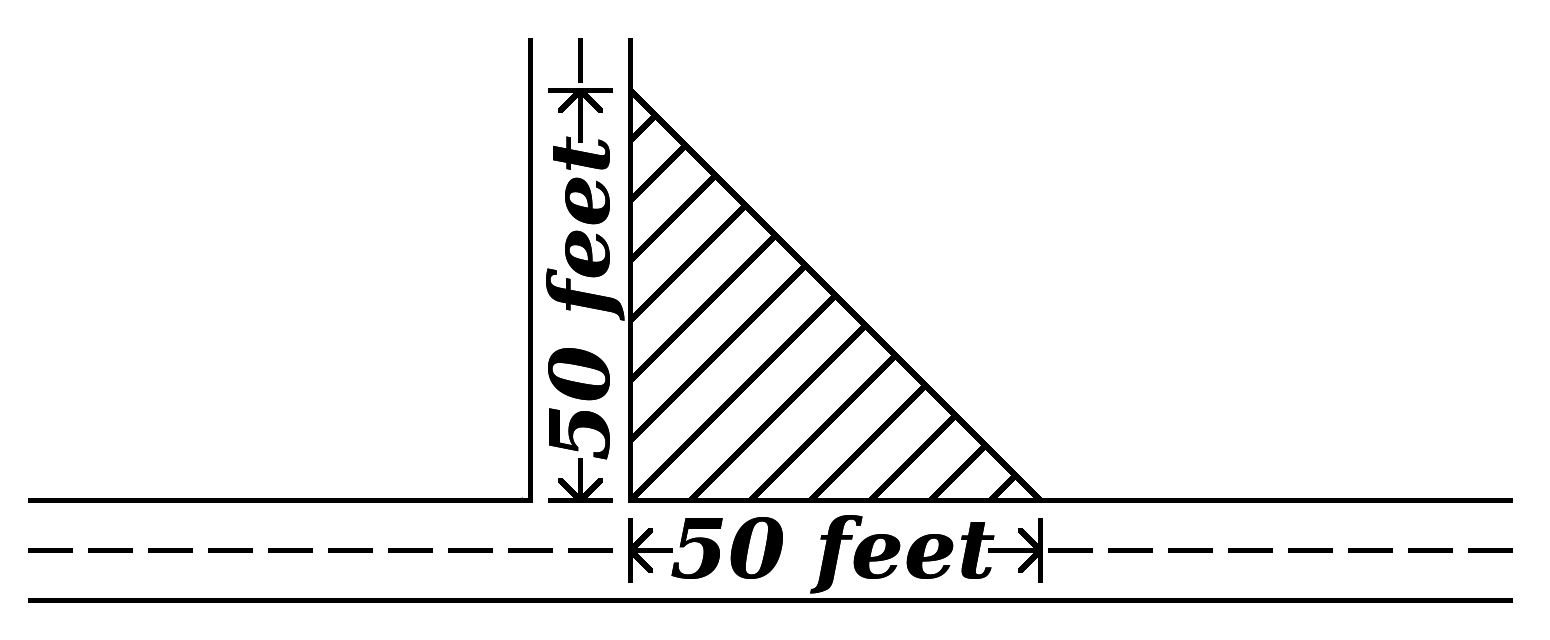
\includegraphics[width=\textwidth]{./images/citycode_fig1.jpg}
    \caption{No obstruction in shaded area of clean sight triangle.}
\end{figure}
\subsection{}
Whenever any street, alley, easement or public way is vacated by official action, the zoning district abutting the centerline of the said vacated area shall not be affected by the proceeding.\footnote{(‘83 Code, SEC. 11.70, Subd. 18)}
\section{Access Drives and Access}
\subsection{}
Access drives may not be placed closer than five feet to any side or rear lot line.  The number and types of access drives onto major streets may be controlled and limited in the interests of public safety and efficient traffic flow.
\subsection{}
Access drives onto county roads shall require a review by the County Engineer.  The County Engineer shall determine the appropriate location, size, and design of the access drives and may limit the number of access drives in the interest of public safety and efficient traffic flow.
\subsection{}
Access drives to principal structures which traverse wooded, steep, or open field areas shall be constructed and maintained to a width and base material depth sufficient to support access by emergency vehicles. The Zoning Administrator shall review all access drives (driveways) for compliance with accepted community access drive standards. All driveways shall have a minimum width of ten feet with a road strength capable of supporting emergency and fire vehicles.
\subsection{}
All lots or parcels shall have direct physical access for emergency vehicles along the frontage of the lot or parcel from either an existing dedicated public roadway, or an existing private roadway approved by the Council.\footnote{(‘83 Code, SEC. 11.70, Subd. 19)}
\section{Private Sewer Systems}
The standards as found in Minnesota Pollution Control Agency’s Standards for Sewage Treatment Systems (6 MCAR 4.8040) are hereby adopted by reference. If there are any inconsistencies between the standards found in this chapter and the state standards, or in 6 MCAR 4.8040 amended, the state standards shall govern.\footnote{(‘83 Code, SEC. 11.70, Subd. 20)}\footnote{\textbf{Note:} If a mobile home park is converted to another use requiring a variance or zoning change, the Planning Commission must give notice of hearing to each occupant. See M.S. \textsection 3270.095, as it may be amended from time to time.}\\
\section{Mobile Home Parks}
\subsection{Purpose}
The purposes of this section are to promote health, safety, order, convenience and general welfare by establishing minimum standards for mobile home parks, the location and use of mobile homes and the design, construction, alteration and arrangement of homes on said lots, authorizing the inspection of mobile home parks, and fixing penalties for violations thereof.
\subsection{Permits}
\subsubsection{}
It is unlawful for any person to place or maintain any mobile home park on any premises except in the R-2 and R-3 Zoning Districts.
\subsubsection{}
It is unlawful for any person to construct, alter, or extend any mobile home park or structures within the park that are permanent in nature within the limits of the city unless he or she holds a valid permit issued by the Building Inspector in the name of the person for the specific construction, alteration or extension proposed, where permanent means structures that are not on wheels or mobile.
\subsubsection{}
All applications for permits shall contain the following: name and address of applicants, location and legal description of the mobile home but not limited to the following: the area and dimensions of the tract of land; topography sketch of the land; the number, location and size of all mobile home lots; the location and width of internal streets and walkways, the location of water and sewer lines and riser pipes; plans and specifications of the water supply and refuse and sewage disposal facilities; plans and specifications of all buildings constructed or to be constructed within the mobile home park; the location and details of lighting and electrical systems; a landscaping plan; and park ground area and recreation equipment.
\subsection{Review of Applications}
The Planning Commission shall review all applications which shall include a lot layout map and shall hold the hearings as it may deem proper with respect thereto. The finding and recommendations of the Planning Commission shall be forwarded to the Council for appropriate action.
\subsection{Inspection of Mobile Home Parks}
\subsubsection{}
The Zoning Administrator is hereby authorized and directed to make the inspections as are necessary to determine satisfactory compliance with this chapter, including the power to enter at reasonable times upon any private or public property for said purposes.
\subsubsection{}
The Building Inspector, the Chief of Police, or their duly authorized representative, shall have the power to inspect the register containing a record of all residents of the mobile home park.
\subsubsection{}
It shall be the duty of every occupant of a mobile home park to give the owner thereof or his or her agent or employee access to any part of the mobile home park at reasonable times for the purpose of making the repairs or alterations as are necessary to effect compliance with this chapter.
\subsection{Environmental, Open Space and Access Requirements}
\subsubsection{General Requirements}
Condition of soil, ground water level, drainage, topography shall not create hazards to the property or the health and safety of the occupants. The site should not be exposed to objectionable smoke, noise, odors, or other adverse influences, and no portion subject to unpredictable or sudden flooding.
\subsubsection{Area}
Minimum total mobile park area shall be ten acres.
\subsubsection{Soil and Ground Cover Requirements}
Exposed ground surfaces in all parts of every mobile home park shall be paved or covered with stone, screenings or other solid material, or protected with a grass that is capable of preventing soil erosion and of eliminating objectionable dust.
\subsubsection{Site Drainage Requirements}
The ground surface in all parts of every mobile home park shall be graded and equipped to drain all surface water in a safe, efficient manner.
\subsubsection{Use Requirements}
\begin{enumerate}[{\indent}a)]
    \item No part of any park shall be used for non-residential purposes, except the uses that are required for the direct servicing and well being of park residents and for the management and maintenance of the park; and 
    \item Nothing contained in this subchapter shall be deemed as prohibiting the sale of a mobile home located on a mobile home stand and connected to the pertinent utilities.
\end{enumerate}
\subsubsection{Required Separation between Mobile Homes}
\begin{enumerate}[{\indent}a)]
    \item Mobile homes shall be separated from each other and from other buildings and structures by at least 15 feet. Mobile homes placed end-to-end must have minimum clearance of 15 feet; 
    \item An accessory structure such as an awning, cabana, storage cabinet, carport, windbreak, and porch which has an opaque top or roof, shall, for purposes of all separation requirements, be considered to be part of the mobile home; and 
    \item Minimum lot sizes shall not be less than 5,000 square feet.
\end{enumerate}
\subsubsection{Open Space}
A minimum of 500 square feet per mobile home shall be provided for definable play areas and open space within the mobile home park. The areas of open space and play area shall not be areas included within any setback nor shall they include any areas of less than 20 feet in length or width.
\subsubsection{Required Setbacks, Buffer Strips and Screenings}
\begin{enumerate}[{\indent}a)]
    \item All mobile homes shall be located at least 30 feet from any property boundary line abutting upon a public street or highway and at least 30 feet from other property boundary lines; 
    \item There shall be a minimum distance of 25 feet between the mobile home stand and abutting park street; and 
    \item All mobile home parks located adjacent to residential, recreational, commercial or industrial land uses shall provide screening such as fences, shrubs, trees, along the property boundary line separating the park and the uses, and shall be maintained by state license holder in a neat and orderly manner.
\end{enumerate}
\subsubsection{Cluster Development}
Cluster development shall be encouraged; in these cases the Planning Commission and Council may vary or modify the strict application and requirements of divisions (E)(6), (7) and (8) above, as applied herein to more readily accommodate this development concept.
\subsubsection{Maximum Density}
Notwithstanding the type of development concept used, the maximum density shall be six mobile homes per acre.
\subsubsection{Storage Buildings}
\begin{enumerate}[{\indent}a)]
    \item One storage building for storage of equipment and refuse is permitted by occupant; and 
    \item The storage buildings shall be designed of weather resistance material that will enhance the general appearance of the lot.
\end{enumerate}
\subsection{Park Street System and Car Parking}
\subsubsection{General Requirements}
All mobile home parks shall be provided with safe and convenient vehicular access from abutting public streets or roads to each mobile home lot.
\subsubsection{Internal Streets}
Surfaced roadways shall be of adequate width to accommodate anticipated traffic, and in any case shall meet the following requirements:
\begin{enumerate}[{\indent}a)]
    \item All park streets shall be a minimum of 30 feet in width from face of curb to face of curb.  Streets without curb shall be considered minor streets.
    \item Minor streets shall be a minimum of 18 feet in width and limited in length to 500 feet.
    \item Dead-end streets shall be provided at the closed end with a reasonable turning area.  All dead-end streets shall be marked with approved signs at the entrance.
\end{enumerate}
\subsubsection{Car Parking}
Off-street parking areas for the use of park occupants and guests. The areas shall be furnished at a rate of at least two car spaces for each mobile home lot, of which at least ${^1/_2}$ of the spaces may be in compounds. Driveways and parking lots shall be paved concrete or bituminous surface. At least one space will be provided on driveway.
\subsubsection{Required Illumination of Park Street Systems}
All parks shall be furnished with lighting units so spaced and equipped with luminaries placed at the mounting heights as will provide average levels of illumination.
\subsubsection{Street Construction and Design Standards}
\paragraph{Pavements}
All park streets shall be provided with a paved concrete or bituminous surface.
\paragraph{Intersections}
Within 50 feet of an intersection, streets shall be at right angles.
\subsection{Walks}
All mobile home stands shall be provided with safe, convenient, all-season pedestrian access of adequate width for indented use.
\subsection{Trees}
A minimum of one tree per lot is required. In open area and park area, a minimum of 20 trees per acre is required.
\subsection{Skirts}
All mobile homes shall have skirts around the entire mobile home made of metal, plastic, fiberglass or comparable, non-combustible material approved by the Building Inspector and shall be painted to match the appropriate mobile home so that it will enhance the general appearance thereof.
\subsection{Water and Sewage}
All mobile homes shall be serviced by the city water system, or a water system approved by the city, and by the city sanitary sewer system.
\subsection{Refuse Handling}
The storage, collection and disposal of refuse in the mobile home park shall be so conducted as to create no health hazards, rodent harborage, insect breeding, accident or fire hazards or air pollution, according to city regulations.
\subsection{Fire Protection}
\subsubsection{Litter, Rubbish, and the Like}
Mobile home parks shall be kept free of litter, rubbish and other inflammable material, and state license holder shall be held liable.
\subsubsection{Fire Extinguishers}
Portable fire extinguishers rated for Classes A, B and C fires shall be kept visible in service buildings and at other locations conveniently and readily accessible for use by all of the occupants and shall be maintained in good operating condition. Their capacity shall not be less than ten pounds.
\subsubsection{Fires}
Fires shall be made only in stoves, indoor approved incinerators, and other equipment intended for those purposes.
\subsubsection{Hydrants}
Fire hydrants shall be installed.  
\begin{enumerate}[{\indent}a)]
    \item The water supply system shall permit the operation of standard city fire hydrants; and 
    \item Fire hydrants shall be located within 300 feet of any mobile home, service building or other structure in the park.
\end{enumerate}
\subsection{Responsibilities of the Park Management}
\subsubsection{}
The person to whom a license for a mobile home park is issued shall operate the park in compliance with this chapter and shall provide adequate supervision to maintain the park, its facilities and equipment in good repair and in a clean and sanitary condition.
\subsubsection{}
The park management shall notify park occupants of all applicable provisions of this chapter and inform them of their duties and responsibilities under this chapter.
\subsubsection{}
It shall be the duty of the operator of the mobile home park to keep a register containing a record of all mobile home owners and occupants located within the park. The register shall contain the following information: The name and address of each mobile home occupant, the name and address of the owner of each mobile home and motor vehicle by which it is towed; the make, model, year and license number of each mobile home and motor vehicle, the state, territory or country issuing the license; and the date of arrival and departure of each mobile home.
\subsubsection{}
The park shall keep the register available for inspection at all times by law enforcement officers, public health officers, and other officials whose duty necessitates acquisition of the information in the register. The register record for each occupant registered shall not be destroyed for a period of three years of the registrant from the park.\footnote{(‘83 Code, SEC. 11.70, Subd. 21)}
\section{Off-Street Parking}
\subsection{Location}
All accessory off-street parking facilities required herein shall be located as follows:
\begin{enumerate}[{\indent}1)]
    \item Spaces accessory to one and two-family dwellings on the same lot as the principal use served.
    \item Spaces accessory to the multiple family dwellings on the same lot as the principal use served or within 200 feet of the main entrance to the principal building served.
    \item Spaces accessory to uses located in a business, within 800 feet of a main entrance to the principal building served.
    \item There shall be no off-street parking space within five feet of any street right-of-way.
    \item No off-street open parking area containing more than four parking spaces shall be located closer than five feet from an adjacent lot zoned or used for residential purposes.
\end{enumerate}
\subsection{General Provisions}
\begin{enumerate}[{\indent}1)]
    \item Access drives may be placed adjacent to property lines except that drives consisting of crushed rock, or other non-finished surfacing shall be no closer than five feet to any side or rear lot line.
    \item Each parking space shall not be less than nine feet wide and 20 feet in length.
    \item When required, accessory off-street parking facilities are provided elsewhere than on the lot in which the principal use served is located, they shall be in the same ownership or control, either by deed or long-term lease, as the property occupied by the principal use, and the owner of the principal use shall file a recordable document with the Council requiring the owner and his or her heirs and assigns to maintain the required number of off-street spaces during the existence of said principal use.
    \item Required off-street parking space in any district shall not be utilized for open storage of goods or for the storage of vehicles which are inoperable or for sale or rent.
    \item Parking shall not be allowed in areas not designated for off-street parking.
\end{enumerate}
\subsection{Design and Maintenance of Off-Street Parking Areas}
\subsubsection{Access}
Parking areas shall be designed so as to provide adequate means of access to a public alley or street. The driveway access shall not exceed 30 feet in width and shall be so located as to cause the least interference with traffic movement.
\subsubsection{Curbing and Landscaping}
All open off-street parking areas designed to have head-in parking along the property line shall provide a bumper curb not less than five feet from the side property line or a guard of normal bumper height not less than three feet from the side property line.  When said area is for six spaces or more, a curb or fence not over five feet in height shall be erected along the front yard setback line and grass or planting shall occupy the space between the sidewalk and curb or fence.
\subsubsection{Parking Space for Six or More Cars}
When a required off-street parking space for six cars or more is located adjacent to a residential district, a fence approved by the Building Official shall be erected along the residential district property line.
\subsubsection{Maintenance of Off-Street Parking Space}
It shall be the joint and several responsibility of the operator and owner of the principal use, uses and/or building to maintain, in a neat and adequate manner, the parking space, accessways, landscaping and required fences.
\subsubsection{Determination of Areas}
A parking space shall not be less than 300 square feet per vehicle of standing and maneuvering area.
\subsection{Other Parking in Residential Areas}
Parking in residential areas (off-street and on-street) shall be limited to the use of the residents of those homes. Except for short-term parking (eight hours or less), guest parking, and vehicles parked in a garage or carport, the number of vehicles parked on or in front of a residential lot shall not exceed one greater than the number of persons residing on the premises and having automobile driver’s licenses.
\subsection{Off-Street Spaces Required (One Space Equals 300 Square Feet)}
\subsubsection{One and Two-Family Residences}
Two spaces per dwelling unit.
\subsubsection{Multiple Dwellings}
One and one-half spaces per dwelling unit.
\subsubsection{Business and Professional Offices}
One space for each 200 square feet of gross floor space.
\subsubsection{Medical and Dental Clinics}
Five spaces for doctor or dentist, plus one space for each employee.
\subsubsection{Hospitals and Sanitoriums}
At least one parking space for each three hospital beds, plus one space for each four employees, other than doctors, plus one parking space for each resident and regular staff doctor.
\subsubsection{Educational Institutions}
\paragraph{Pre-Schools and Elementary Schools}
One space for each two employees.
\paragraph{Junior and Senior High Schools}
One space for each two faculty and full-time employees plus one space for each seven students.
\paragraph{Colleges and Universities}
Same as for high school except one space for each five students.
\paragraph{Auditoriums, Stadiums}
One space for each six seats.
\subsubsection{Drive-In Food Establishments}
One space for each 15 square feet of gross floor space in building allocated to drive-in operation.
\subsubsection{Bowling Alley}
Six spaces for each alley, plus additional spaces as may be required herein for related uses such as a restaurant.
\subsubsection{Automobile Service Station}
At least two off-street parking spaces plus four off-street parking spaces for each service stall.
\subsubsection{Hotel or Motel}
One space per rental unit plus one space per full-time employee.
\subsubsection{Retail Store}
At least one off-street parking space for each 250 square feet of gross floor area.
\subsubsection{Restaurants, Cafes, Bars, Taverns, Night Clubs}
At least one space for each three seats based on capacity design.
\subsubsection{Undertaking Establishments}
Eight spaces for each chapel or parlor, plus one space for each funeral vehicle maintained on the premises. Aisle space shall also be provided off the street for making up a funeral procession.
\subsubsection{Industrial, Warehouse, Storage, Handling of Bulk Goods}
At least one space for each employee on maximum shift or one space for each 2,000 square feet of gross floor area, whichever is larger.
\subsubsection{Churches, Chapels, Temples, Synagogues}
One parking space for each six seats.
\subsubsection{Uses not Specifically Noted}
As determined by the Council following review by the Planning Commission.
\subsubsection{}
Within the Central Business District (C-1), the Zoning Administrator may authorize a number of parking spaces lower than the number generally required. When determining the number of parking spaces required, the Zoning Administrator shall require the property owner or operator to identify the time and days of operation of the subject use, the maximum number of employees and the expected number of clients or customers. In addition to the information provided by the property owner or operator, the Zoning Administrator shall consider the characteristics of existing like land uses, the number and characteristics of the businesses in the area of the subject use and the availability of additional private parking development. A record of the decision of the Zoning Administrator shall be kept on file in the office of the City Building Official.
\subsection{Off-Street Loading and Unloading Areas}
\subsubsection{Location}
All required loading berths shall be off-street and shall be located on the same lot as the building or use to be served. A loading berth shall be located at least 25 feet from the intersection of two street rights-of-way and at least 50 feet from a residential district unless within a building.  Loading berths shall not occupy the required front yard space.
\subsubsection{Size}
Unless otherwise specified in this chapter, a required loading berth shall be not less than 12 feet in width, 50 feet in length and 14 feet in height, exclusive of aisle and maneuvering space.\footnote{(Ord. 537, effective 7-1-83)}
\subsubsection{Required Loading Spaces}
Determined by the Building Official.\footnote{(Ord. 42, 2nd Series, effective 4-23-87)}
\subsubsection{Access}
Each required loading berth shall be located with appropriate means of vehicular access to a street or public alley in a manner which will least interfere with traffic.
\subsubsection{Surfacing}
All loading berths and accessways shall be improved with a durable material to control the dust and drainage.
\subsubsection{Accessory Use}
Any space allocated as a loading berth or maneuvering area so as to comply with the terms of this chapter shall not be used for the storage of goods, inoperable vehicles or be included as a part of the space requirements necessary to meet the off-street parking area.
\subsubsection{}
In connection with any structure which is to be erected or substantially altered, and which requires the receipt or distribution of materials or merchandise by trucks or similar vehicles, there shall be provided off-street loading space.
\subsubsection{}
Where noise from loading or unloading activity is audible in a residential district, the activity shall terminate between the hours of 7:00 p.m. and 7:00 a.m.\footnote{(‘83 Code, SEC. 11.70, Subd. 22)}
\section{Auto Service Station Standards}
\subsection{Lot Size}
A service station site shall be a minimum of 20,000 square feet in size.
\subsection{Setbacks}
The building or buildings shall be set back at least 35 feet from the street right-of-way. Near residential districts, the service station buildings, signs, and pumps shall be a minimum of 25 feet from adjoining property. In commercial areas, the structures shall be set back at least ten feet from adjoining property.
\subsection{Curbs and Gutters}
Curbs and gutters shall be installed on all streets giving access to the station. There shall be a six inch curb along all interior driveways.
\subsection{Fencing and Screening}
When adjacent to residential property, there shall be a screening fence. When adjacent to commercial property, there shall be a bumper-type fence about 18 inches high between the station and the adjacent commercial property.
\subsection{Vehicles}
No vehicles shall be parked on the premises other than those utilized by employees or awaiting service. No vehicle shall be parked or be waiting service longer than 15 days.
\subsection{Exterior Storage}
Exterior storage besides vehicles shall be limited to service equipment and items offered for sale. Exterior storage of items offered for sale shall be within yard setback and shall be located in containers such as the racks, metal trays, and similar structures designed to display merchandise.
\subsection{Screening}
All areas utilized for the storage or disposal of trash, debris, discarded parts, and similar items shall be fully screened.  All structures and grounds shall be maintained in orderly, clean and safe manner.
\subsection{Architecture}
The station shall be of a design that is compatible with the surroundings.
\subsection{Outdoor Displays}
The storage of used tires, batteries, and other items for sale outside the building shall be controlled; the items shall be displayed in specially designed containers and be limited to one or two areas well back from the right-of-way street line. Junk cars, empty cans, and other unsightly material will not be permitted in an area subject to public view.
\subsection{Other Activities}
\subsubsection{}
Business activities not listed in the definition of service stations and not incidental to the business in this chapter are not permitted on the premises of a service station unless a conditional use permit is obtained specifically for the business. The activities include, but are not limited to, the following:
\begin{enumerate}[{\indent}a)]
    \item Automatic car and truck wash; 
    \item Rental of vehicles, equipment, or trailers; and 
    \item General retail sales.
\end{enumerate}
\subsubsection{}
Gas pumps located at and a part of other types of business establishments shall require a conditional use permit.\footnote{(‘83 Code, SEC. 11.70, Subd. 23)}\footnote{Penalty, see 152.999}
\section{Drive-In Business Standards}
The following standards shall apply to drive-in businesses in all districts.
\subsection{Drainage System}
The entire area of any drive-in business shall have a drainage system approved by the City Engineer.
\subsection{Surface}
The entire area other than that occupied by structures or planting shall be surfaced with a hard surface material which will control dust and drainage.
\subsection{Fence or Screen}
A fence or screen of acceptable design not over six feet in height or less than four feet shall be constructed along the property line abutting a residential district and the fence or screen shall be adequately maintained.
\subsection{General}
\begin{enumerate}[{\indent}1)]
    \item Any drive-in business serving food or beverages may also provide, in addition to vehicular service areas, indoor food and beverage service seating area.
    \item The hours of operation shall be set forth as a condition of any building permit for drive-in business.
    \item Each drive-in business serving food may have outside seating.
    \item Each food or beverage drive-in business shall place refuse receptacles at all exits as well as one refuse receptacle per ten vehicle parking spaces within the parking area.
\end{enumerate}
\subsection{Locations}
\begin{enumerate}[{\indent}1)]
    \item No drive-in business serving food or beverage shall be located within 100 feet of a public or parochial school, church or any residential dwelling unit.
    \item No drive-in shall be located on any street other than one designated as a thoroughfare or business service road in the Comprehensive Plan.
\end{enumerate}
\subsection{Site Plan\footnote{(‘83 Code, SEC. 11.70, Subd. 24)}\footnote{(Ord. 537, effective 7-1-83)}}
\begin{enumerate}[{\indent}1)]
    \item The site plan shall clearly indicate suitable storage containers for all waste material.  All commercial refuse containers shall be screened.
    \item A landscaping plan shall be included and shall set forth complete specifications for plant materials and other features.
    \item Adequate area shall be designated for snow storage so that clear visibility shall be maintained from the property to any public street.
    \item The design of any structure shall be compatible with other structures in the surrounding area.
    \item Electronic devices such as loudspeakers, automobile service order devices, drive-in theater car speakers and similar instruments shall not be located within 300 feet of any residential unit.
    \item No service shall be rendered, deliveries made, or sales conducted within the required front yard; customers served in vehicles shall be parked to the sides and/or rear of the principal structure.
    \item No access drive shall be within 50 feet of intersecting street curb lines.
    \item In the case of a drive-in theater, a solid fence not less than eight feet in height and extending at least to within two feet of the ground shall be constructed around the property.
    \item The lighting shall be designed so as to have no direct source of light visible from the public right-of-way or adjacent land in residential use.
\end{enumerate}


\section{Signs}
\subsection{Purpose}
The purpose of this section is to provide for necessary visual communication, to preserve and promote a pleasant physical environment, to protect public and private property, and to encourage safety upon the streets and highways within the city for regulating the structure, size, location, height, lighting, and the erection and maintenance of all outdoor signs and sign structures within the city.
\subsection{Signs Requiring No Permit}
The following signs are authorized everywhere within the city and shall not require a permit for their erection or maintenance:
\begin{enumerate}[{\indent}1)]
    \item Public signs.
    \item Memorial signs.
    \item Real estate signs.
    \item Signs that are not visible from any road or from any residential district.
\end{enumerate}
\subsection{Prohibited Signs}
It is unlawful for any person to erect or maintain any sign which is prohibited or is not specifically authorized under this section including, but not limited to:
\begin{enumerate}[{\indent}1)]
    \item Signs that, by reason of position, shape, color, or illumination, would interfere with the proper function of traffic signs or signals.
    \item Signs that resemble any official marker erected by a government agency or that display the words as “Stop" or “Danger" and are not placed by a governmental agency or its agent. L
    \item Flashing signs, except where specifically authorized under this section.
    \item Billboard signs.
    \item Advertising signs,ie'xcept where specifically authorized under this section.
    \item Except as specifically authorized by conditional use permit under provisions contained elsewhere in this section, off-premise signs.
    \item Roof signs.
    \item Projecting signs.
    \item Portable signs, except Where specifically authorized under this section.
    \item Temporary signs.
    \item Changeable copy signs, except where specifically authorized under this section.
    \item Any sign which is operated or maintained in conjunction with sound.
\end{enumerate}
\subsection{Historic District}
\subsubsection{Authorized Signs\footnote{(Ord. 85, 2nd Series, effective 7-17-93)}}
The following signs are authorized in the Historic District and require a permit for their erection or maintenance:
\begin{enumerate}[{\indent}a)]
    \item Awning signs that are identification signs.
    \item Marquee signs that are identification signs.
    \item Wall signs that are identification signs.
\end{enumerate}
\subsubsection{Performance Standards}
\paragraph{Size and Location}
Maximum sign surface height shall be 36 inches and sign length shall be limited to 50\% of the associated building face.\footnote{(Ord. 90, 2nd Series, effective 5-14-94)}
\paragraph{Materials}
Materials used for the sign structure should have a reasonable degree of consistency and reflect a sense of concern for the visual amenities within the Historic District, yet encourage creativity and opportunity for effective communication.
\paragraph{Design Review}
Signs requiring a permit may be submitted to the Planning Commission, the Crookston 2000 Design Team, or other appropriate group for review and comment.  Permits may be withheld until sign plans are consistent with design review recommendations.
\subsection{Residential Districts (R-1, R-2, and R-3)}
\subsubsection{Authorized Signs}
The following signs are authorized in the R-1, R-2, and R-3 Zoning Districts and require a permit for their erection or maintenance:
\begin{enumerate}[{\indent}a)]
    \item Home occupation signs that are either wall signs or grounds signs.
    \item Identification signs that are ground signs.
\end{enumerate}
\subsubsection{Performance Standards}
Ground signs shall have a maximum height of three feet and an area of 2 ½ feet for home occupation signs and a maximum height of nine feet and an area of 25 feet for identification signs and both types of signs must be set back from property lines at least ten feet.
\subsection{Central Business District (C-1)}
\subsubsection{Authorized Signs}
The following signs are authorized in that portion of the C-1 Zoning District which is not within the Historic District and require a permit for their erection or maintenance:
\begin{enumerate}[{\indent}a)]
    \item Awning signs.
    \item Marquee signs.
    \item Wall signs.
    \item Ground signs.
    \item Pole signs.
    \item Flashing sign, except those which outside of the message area.
    \item Changeable copy signs.
    \item Off-premise signs when authorized by conditional use permit upon a finding of the Council, among other required findings, that such off-premise sign promotes the public health, safety, and general welfare.
\end{enumerate}
\subsubsection{Performance Standards}
\paragraph{Size and Location}
Requirements for wall signs shall be the same as for the Historic District.  Ground signs may be placed on parcels having minimum public street frontage of 100 feet and minimum building set back of 25 feet.  Ground signs shall have maximum sign area of 50 square feet and height of nine feet.
\paragraph{Pole Signs}
Pole signs may be considered only when because of obstruction of sight lines or for other reasons a ground sign is not feasible.  If allowed, pole signs shall have a maximum sign area of 50 square feet and height of ten feet above street level to bottom of sign.
\paragraph{Changeable Copy, Flashing or Illuminated Signs}
Only one changeable copy or flashing sign shall be allowed per business, lot or parcel. Nighttime intensity must be reduced to 50\% of daytime intensity for illuminated signs which are illuminated during both the daytime and nighttime.
\subsection{Highway Business District (C-2), Shopping Center District (C-3), Heavy Industry District (I-1), Light Industry District (I-2), and Institutional District (IN)}
\subsubsection{}
The following signs are authorized in the C-2, C-3, I-1, I-2 and IN Zoning Districts and a permit is required for their erection or maintenance:
\begin{enumerate}[{\indent}a)]
    \item Awning signs.
    \item Marquee signs.
    \item Wall signs.
    \item Ground signs.
    \item Pole signs.\footnote{(Ord. 85, 2nd Series, effective 7-17-93)}
    \item Portable signs that are advertising signs located on the premises to which they have reference.\footnote{(Ord. 93, 2nd Series, effective 9-17-94)}
    \item Flashing signs, except those which “flash" outside of the message area.
    \item Changeable copy signs.
    \item Off-premise signs when authorized by conditional use permit upon a finding of the Council, among other required findings, that such off-premise sign promotes the public health, safety, and general welfare.
\end{enumerate}
\subsubsection{Performance Standards}
\paragraph{Size and Location\footnote{(Ord. 85, 2nd Series, effective 7-17-93)}}
Requirements for wall signs shall be the same as for the Historic District, except maximum sign surface height shall be one-third of building height. Requirements for ground and pole signs are as follows:
\begin{center}
    \begin{tabular}{| c | >{\centering\arraybackslash}m{2.5cm} | c | >{\centering\arraybackslash}m{2.5cm} | >{\centering\arraybackslash}m{2.5cm} |}
    \hline
    \emph{\textbf{Speed Zone}} & \emph{\textbf{Setback from Center of Right-of-Way}} & \emph{\textbf{Max. Sq. ft.}} & \emph{\textbf{\mbox{Max. Height} \mbox{(in ft.)} \mbox{Ground Sign}}} & \emph{\textbf{Height \mbox{(in ft.)} \mbox{Pole Sign}}}\\
    \hline
    30 & 100 ft. \mbox{or less} & 75 & 9 & min. 10; \mbox{max. 20}\\
    \hline
    30 & more than \mbox{100 ft.} & 100 & 9 & min. 10; \mbox{max. 20}\\
    \hline
    45 & 100 ft. \mbox{or less} & 100 & 9 & min. 12; \mbox{max. 25}\\
    \hline
    45 & more than \mbox{100 ft.} & 125 & 11 & min. 12; \mbox{max. 25}\\
    \hline
    55 & 100 ft. \mbox{or less} & 125 & 11 & min. 12; \mbox{max. 30}\\
    \hline
    55 & more than \mbox{100 ft.} & 150 & 11 & min. 12; \mbox{max. 30}\\
    \hline
\end{tabular}
\end{center}
\paragraph{Number}
Wall signs are limited to one per building face. Only one ground sign or pole sign will be allowed per business or lot, except that a total of two ground or pole signs will be allowed if the lot involved has at least 200 lineal feet of frontage.\footnote{(Ord. 90, 2nd Series, effective 5-14-94)}
\paragraph{Portable Signs}
Portable signs may be permitted for each special event for up to 15 continuous days for a grand opening and up to seven continuous days for other special events, including, but not limited to, open houses and special sales. The sign placement dates will be stated on the permit. Applicants are limited to ten portable sign permits per calendar year. It is unlawful for the applicant to which a portable sign permit is issued to maintain or fail to remove a portable sign after the permit time has expired.\footnote{(Ord. 93, 2nd Series, effective 9-17-94)}
\paragraph{Changeable Copy, Flashing or Illuminated Signs}
Only one changeable copy or flashing sign shall be allowed per business, lot or parcel. Nighttime intensity must be reduced to 50\% of daytime intensity for illuminated signs which are illuminated during both the daytime and nighttime.
\subsection{Farm Residence District (FR)}
Except for signs which are otherwise authorized, any signs erected or maintained in the FR Zoning District must have a conditional use permit for the erection and maintenance.
\subsection{Nonconforming Signs}
\subsubsection{Continued}
An existing sign which is lawful at the time of the adoption of a relevant part of this section may be continued, even if the sign does not conform to the regulations of this section, except as provided below.
\subsubsection{Extension}
A nonconforming sign may not be enlarged or changed so as to increase its nonconformity.
\subsubsection{Relocation}
A nonconforming sign may not be moved unless it then conforms to the requirements of this section.
\subsubsection{Vacation/Change of Ownership}
If the premises upon which a nonconforming sign is located is abandoned or vacated or if the ownership of the premises or nonconforming sign changes, the nonconforming sign must be removed or brought into full compliance with this section.
\subsubsection{Repairs/Maintenance}
Normal maintenance of a nonconforming sign is authorized and required, including necessary non-structural repairs and incidental alterations which do not extend or intensify the nonconformity. Repairs costing in excess of 50\% of the nonconforming sign’s replacement cost are not authorized. Any improvements to the parcel of land to which a nonconforming sign relates which cost over \$10,000 or more than 50\% of the market value of the existing improvements thereon shall require that the nonconforming sign is removed or brought into compliance with this section.
\subsubsection{Inspection}
The enforcing officer may make inspections of all nonconforming signs and may enter upon or in the premises at reasonable hours for inspection purposes.
\subsection{Maintenance/Inspection}
All signs must be properly maintained so as to remain legible and free of peeling paint and loose or missing components. No sign shall be misleading to the public, such as, for example, a sign referring to a business which is no longer on the premises. The enforcing officer may make inspections of all signs and may enter upon or in the premises at reasonable hours for inspection purposes.
\subsection{Abatement}
If the enforcing officer finds that any sign has been erected or is being maintained in violation of this section or that any sign is inadequately maintained or presents a safety hazard, the enforcing officer will give written notice of the violation to the installer of the sign and to the owner or manager of the property upon which the sign exists. If, after receiving notice, the sign is not removed or altered as required, the sign shall be deemed a public health or safety hazard and may be abated by the city under SEC. 94.01 of the city code.\footnote{(Ord. 85, 2nd Series, effective 7-17-93)}\footnote{(‘83 Code, SEC. 11.70, Subd. 25)  Penalty, see 152.999}
\section{Home Occupations}
\subsection{Definition} A \textbf{HOME OCCUPATION} is any gainful occupation or profession engaged in by the occupant of a dwelling at or from the dwelling when carried on within a dwelling unit or accessory structure.
\subsection{General Regulations\footnote{(‘83 Code, SEC. 11.70, Subd. 26)}\footnote{Penalty, see 152.999}}
Customary home occupations shall be allowed in the R-1, R-2 and R-3 Districts if they meet the following conditions:
\begin{enumerate}[{\indent}1)]
    \item Not more than 25\% of the gross floor area of the residence is used for this purpose.
    \item Only articles made or originating on the premises shall be sold on the premises, unless the articles are incidental to a permitted commercial service.
    \item No articles for sale shall be displayed so as to be visible from any street.
    \item No person is employed other than a member of the household residing on the premises.
    \item No mechanical or electrical equipment is used if the operation of the equipment interferes unreasonably with the desired quiet residential environment of the neighborhood and the health and safety of the residents is endangered.
    \item The occupation does not generate more than two customer/client vehicles at one time.
    \item The occupation must provide off-street parking for vehicles generated by the occupation.
    \item A person having a home occupation shall provide proof of meeting the above seven requirements if complaints are received by the Council.
\end{enumerate}
\section{Manufactured Homes\footnote{(‘83 Code, SEC. 11.70, Subd. 27)  (Ord. 537, effective 7-1-83)}}
Manufactured homes shall be permitted in the R-1, R-2 and R-3 Districts, provided they meet the following minimum standards:
\begin{enumerate}[{\indent}A)]
    \item Exceeds 24 feet in width.
    \item Has a minimum floor area of 800 square feet.
    \item The dwelling is placed on a permanent foundation.
    \item All other requirements of law and city code provisions are met.
\end{enumerate}
\section{Satellite Dish Antennas\footnote{(Ord. 27, 2nd Series, effective 3-20-86)}\footnote{(‘83 Code, SEC. 11.70, Subd. 28)}\footnote{Penalty, see 152.999}}
Satellite dish antennas shall meet the following minimum standards:
\begin{enumerate}[{\indent}A)]
    \item No satellite dish antenna or portion thereof shall be constructed:
        \begin{enumerate}[{\indent\indent}1)]
            \item In any front yard or within that portion of any side yard which is forward of the front line extended of any existing building upon the lot or parcel involved;
            \item Within the side yard or rear yard set back requirements for accessory structures; 
            \item Upon the roof of any residential dwelling for four or fewer families, private garage, or other structure accessory to the residential dwelling; or 
            \item To exceed the height of 35 feet or the top of the principal structure on the lot upon which it is located, whichever is less.
        \end{enumerate}
    \item Wiring between the satellite dish antenna and a receiver shall be placed at least eight inches beneath the surface of the ground.
    \item Satellite dish antennas shall be bonded to a grounding rod and shall be designed to withstand a wind force as required by the building code.
    \item Satellite dish antennas which are mounted on the roof of a building or structure must be approved by a registered engineer or architect.
\end{enumerate}
\section{Bed and Breakfast Inns\footnote{(Ord. 37, 2nd Series, effective 9-16-86)}\footnote{(‘83 Code, SEC. 11.70, Subd. 29)}\footnote{Penalty, see 152.999}}
Bed and breakfast inns shall meet the following minimum standards:
\begin{enumerate}[{\indent}A)]
    \item Employees shall be limited to the following:
        \begin{enumerate}[{\indent\indent}1)]
            \item Members of the household residing on the premises; and 
            \item One person in a part-time capacity.
        \end{enumerate}
    \item Signs must comply with the sign requirements for home occupations.
    \item On-site, off-street parking must be provided as follows: 
        \begin{enumerate}[{\indent\indent}1)]
            \item One space for each lodging room; and 
            \item One space for the owner.
        \end{enumerate}
    \item The establishment must comply with State of Minnesota Health and Building/Fire Code requirements.
\end{enumerate}

\subchapter{ADMINISTRATION AND ENFORCEMENT}

\setcounter{section}{194}
\section{Enforcing Officer\footnote{(‘83 Code, SEC. 11.15, Subd. 1)}}
The Zoning Administrator and/or Building Official shall enforce this chapter and shall perform the following duties:
\begin{enumerate}[{\indent}A)]
    \item Issue occupancy, building and other permits, and make and maintain records thereof.
    \item Conduct inspections of buildings and use of land to determine compliance with the terms of this chapter.
    \item Maintain permanent and current records of this chapter, including but not limited to, all maps, amendments, and conditional uses, variances, appeals and applications therefor.
    \item Receive, file and forward all applications for appeals, variances, conditional uses or other matters to the designated official bodies.
    \item Notify the City Attorney of any violations of this chapter for appropriate action.
\end{enumerate}
\section{Appeals and Board of Zoning Appeals (See also SEC. 32.130 and SEC. 32.131)}
\subsection{}
A Board of Zoning Appeals is hereby established, which shall consist of the Council, vested with the administrative authority as hereinafter provided.
\subsection{}
The Board of Zoning Appeals shall act upon all questions as they may arise in the administration of this chapter, including the interpretation of zoning maps, and it shall hear and decide appeals from and review any order, requirement, decision, or determination made by the Zoning Administrator. The appeal may be taken by any person, firm, or corporation aggrieved or by any officer, department, board or bureau of the city. The Board of Zoning Appeals shall also have the power to grant variances to the provisions of this chapter under certain conditions indicated in SEC.152.200 of this chapter. No use variances; a use different than that allowed in the zoning district, shall be issued by the Board of Zoning Appeals.
\subsection{}
Meetings by the Board of Zoning Appeals shall be held within the time and upon the notice to interested parties as is provided in this chapter and its adopted rules for the transaction of its business. The Board shall, within 60 days after receiving a request for a variance, refer the proposed variance to the Planning Commission for review and comment. After receiving the comments of the Planning Commission, the Board shall make its order deciding the matter, and shall serve a copy of the order upon the appellant or petitioner by mail. Any party may appear at the meeting in person or by agent or attorney. The Board of Zoning Appeals may reverse or affirm wholly or partially, or may modify the order, requirement, decision, or determination as in its opinion ought to be made and to that end shall have all the powers of the officer from whom the appeal was taken and may issue or direct the issuance of a permit. The reasons for the decision shall be stated and recorded.  The decision of the Board shall not be final and any person having an interest affected by the decision shall have the right to appeal to District Court in the county in which the land is located on questions of law and fact. A vote of the majority of the Board of Zoning Appeals shall be necessary to reverse any decision of an administrative official of the city or to decide in favor of the applicant.\footnote{(‘83 Code, SEC. 11.15, Subd. 2)}
\section{Powers and Duties of Planning Commission (See also SEC. 32.120 and SEC. 32.121)}
\subsection{}
The Planning Commission shall have all the powers and duties defined or granted in the statutes and the city code relating to planning, zoning and subdivision regulations and shall act in an advisory capacity to the Council in all of these areas.\footnote{(‘83 Code, SEC. 2.51, Subd. 2)}
\subsection{}
The Planning Commission shall provide assistance to the Council and Zoning Administrator in the administration of this chapter and the recommendation of the Planning Commission shall be advisory in nature. Specifically, the Planning Commission shall review, hold public hearings, and make recommendations to the Council on all applications for zoning amendments, variances, and conditional use permits using the criteria in SEC. 152.198 through SEC. 152.200 of this chapter.\footnote{(‘83 Code, SEC. 11.15, Subd. 3)}
\section{Zoning Amendments}
\subsection{Criteria for Granting Zoning Amendments}
The Council may adopt amendments to this chapter and the zoning map in relation both to land uses within a particular district or to the location of the district line. The amendments shall not be issued indiscriminately, but shall only be used as a means to reflect changes in the goals and policies of the city as reflected in the Comprehensive Plan or changes in conditions in the city.
\subsection{Kinds of Amendments}
\begin{enumerate}[{\indent}1)]
    \item A change in a district’s boundary (rezoning).
    \item A change in a district’s regulations.
    \item A change in any other provision of this chapter.
\end{enumerate}
\subsection{Initiation of Proceedings}
Proceedings for amending this chapter shall be initiated by at least one of the following three methods:
\begin{enumerate}[{\indent}1)]
    \item By petition of an owner or owners of property which is proposed to be rezoned, or for which district regulation changes are proposed.
    \item By recommendation of the Planning Commission.
    \item By action of the Council.
\end{enumerate}
\subsection{Required Exhibits for Rezoning or District Regulation Changes Initiated by Property Owners}
The following exhibits shall be required unless waived by the Planning Commission or Zoning Administrator.
\begin{enumerate}[{\indent}1)]
    \item A plat map showing property owner’s names and addresses within 350 feet of the outer boundaries of the property in question.
    \item A boundary survey and preliminary building and site development plan.
\end{enumerate}
\subsection{Procedure\footnote{(‘83 Code, SEC. 11.15, Subd. 4)}}
The procedure for a property owner to initiate a rezoning or district regulation change applying to this property is as follows:
\begin{enumerate}[{\indent}1)]
    \item The property owner or his or her agent shall meet with the Zoning Administrator to explain his or her situation, learn the procedures, and obtain an application form.
    \item The applicant shall file the completed application form together with the required exhibits with the Zoning Administrator and shall pay a filing fee as established by the Council.
    \item The Zoning Administrator shall transmit the application and required exhibits to the Planning Commission and shall notify all property owners within the affected zone and within 350 feet of the outer boundaries of the property in question; however, failure of any property owner to receive the notification shall not invalidate the proceedings.
    \item The Planning Commission shall set the date for a public hearing and shall have notices of the hearing published in the legal newspaper at least once, not less than ten days and not more than 30 days prior to said hearing. The Council may waive the mailed notice requirements for a city-wide amendment to this chapter initiated by the Planning Commission or Council.
    \item The Planning Commission shall hold the public hearing and then shall recommend within 60 days, one of three actions: approval, denial or conditional approval.
    \item The Planning Commission shall transmit its recommendations to the Council for its official action within 60 days after holding the public hearing.
    \item The Council shall act upon the application within 60 days after receiving the recommendation of the Planning Commission.
    \item No application of a property owner for an amendment to the text of this chapter or the zoning map shall be considered by the Planning Commission within the one-year period following a denial of the request, except the Planning Commission may permit a new application, if in the opinion of the Planning Commission, new evidence or a change of circumstances warrant it.
\end{enumerate}
\section{Conditional Use Permits}
\subsection{Criteria for Granting Conditional Use Permits}
In granting a conditional use permit, the Council shall consider the advice and recommendations of the Planning Commission and the effect of the proposed use on the Comprehensive Plan and upon the health, safety, and general welfare of occupants of surrounding lands. Among other things, the Council shall make the following findings where applicable.
\begin{enumerate}[{\indent}1)]
    \item The use will not create an excessive burden on existing parks, schools, streets and other public facilities and utilities which serve or are proposed to serve the area.
    \item The use will be sufficiently compatible or separated by distance or screening frown adjacent residentially zoned or used land so that existing homes will not be depreciated in value and there will be no deterrence to development of vacant land.
    \item The structure and site shall have an appearance that will not have an adverse effect upon adjacent residential properties.
    \item The use, in the opinion of the Council, is reasonably related to the overall needs of the city and to the existing land use.
    \item The use is consistent with the purposes of this chapter and the purposes of the zoning district in which the applicant intends to locate the proposed use.
    \item The use is not in conflict with the Comprehensive Plan of the city.
    \item The use will not cause traffic hazard or congestion.
    \item Adequate utilities, access roads, drainage and necessary facilities have been or will be provided.
\end{enumerate}
\subsection{Additional Conditions}
\subsubsection{}
In permitting a new conditional use or the alteration of an existing conditional use, the Council may impose, in addition to these standards and requirements expressly specified by this chapter, additional conditions which the Council considers necessary to protect the best interest of the surrounding area or the community as a whole. These conditions may include, but are not limited to, the following:
\begin{enumerate}[{\indent}a)]
    \item Increasing the required lot size or yard dimension.
    \item Limiting the height, size or location of buildings.
    \item Controlling the location and number of vehicle access points.
    \item Increasing the street width.
    \item Increasing the number of required off-street parking spaces.
    \item Limiting the number, size, location or lighting of signs.
    \item Required diking, fencing, screening, landscaping or other facilities to protect adjacent or nearby property.
    \item Designating sites for open space.
    \item Establishing a time limit for the conditional use.
\end{enumerate}
\subsubsection{}
The Zoning Administrator shall maintain a record of all conditional use permits issued including information on the use, location, and conditions imposed by the Council; time limits, review dates, and the other information as may be appropriate.
\subsection{Required Exhibits for Conditional Use Permits}
The following exhibits shall be required unless waived by the Planning Commission or Zoning Administrator.
\begin{enumerate}[{\indent}1)]
    \item A plat map showing property owner’s names and addresses within 350 feet of the outer boundaries of the property in question.
    \item A boundary survey and preliminary building and site development plan.
\end{enumerate}
\subsection{Procedure\footnote{(‘83 Code, SEC. 11.15, Subd. 5)}\footnote{\textbf{Note:} If a mobile home park is converted to another use requiring a variance or zoning change, the Planning Commission must give notice of hearing to each occupant. See M.S. \textsection 327C.095, as it may be amended from time to time.}}
The procedure for obtaining a conditional use permit is as follows:
\begin{enumerate}[{\indent}1)]
    \item The property owner or his or her agent shall meet with the Zoning Administrator to explain his or her situation, learn the procedures and obtain an application form.
    \item The applicant shall file the completed application form together with the required exhibits with the Zoning Administrator and shall pay a filing fee as established by the Council.
    \item The Zoning Administrator shall transmit the application to the Planning Commission and shall notify all property owners within 350 feet of the outer boundaries of the property in question; however, failure of any property owner to receive the notification shall not invalidate the proceedings.
    \item The Zoning Administrator shall set the date for a public hearing and shall have notice of the hearing published at least once in the legal newspaper, not less than ten days and not more than 30 days prior to said hearing.
    \item The Planning Commission shall hold the public hearing and then shall study the application to determine possible adverse effects of the proposed special use and to determine what additional requirements may be necessary to reduce the adverse effects and recommend one of three actions:  approval, denial, or conditional approval.
    \item The Planning Commission shall transmit, within 60 days, its recommendation to the Council for its official action.
    \item The Council shall take appropriate action on the request for a conditional use permit within 60 days of receiving the recommendations by the Planning Commission. If it grants the conditional use permit, the Council may impose conditions (including time limits) it considers necessary to protect the public health, safety and welfare and the conditions may include a time limit for the use to exist or operate.
    \item Where a conditional use permit has been issued pursuant to the provisions of this chapter, the permit shall become null and void without further action by the Planning Commission or the Council unless work thereon commences within one year of the date of granting the conditional use. A conditional use permit shall be deemed to authorize only one particular use and shall expire if that use shall cease for more than 12 consecutive months.
    \item In the event that the applicant violates any of the conditions set forth in this permit, the Council shall have the authority to revoke the conditional use permit.
\end{enumerate}
\section{Variances}
\subsection{Criteria for Granting Variances}
A variance to the provisions of this chapter may be issued by the Board of Zoning Appeals to provide relief to the landowner in those cases where this chapter imposes undue hardship or practical difficulties to the property owner in the use of his or her land.  No use variances may be issued.  A variance may be granted only in the event that the following circumstances exist:
\begin{enumerate}[{\indent}1)]
    \item Exceptional or extraordinary circumstances apply to the property which do not apply generally to other properties in the same zone or vicinity, and result from lot size or shape, topography, or other circumstances over which the owners of property since enactment of this chapter have had no control.
    \item The literal interpretation of the provisions of this chapter would deprive the applicant of rights commonly enjoyed by other properties in the same district under the terms of this chapter.
    \item That the special conditions or circumstances do not result from the actions of the applicant.
    \item That granting the variance requested will not confer on the applicant any special privilege that is denied by this chapter to owners of other lands, structures or buildings in the same district.
    \item That the variance requested is the minimum variance which would alleviate the hardship.  Economic conditions alone shall not be considered a hardship.
    \item The variance would not be materially detrimental to the purposes of this chapter, or to other property in the same zone.
    \item The proposed variance will not impair an adequate supply of light and air to adjacent property, or substantially increase the congestion of the public streets, or increase the danger of fire, or endanger the public safety, or substantially diminish or impair property values within the neighborhood. The Board of Zoning Appeals may impose the restrictions and conditions upon the premises benefitted by a variance as may be necessary to comply with the standards established by this chapter, or to reduce or minimize the effect of the variance upon other properties in the neighborhood, and to better carry out the intent of the variance.
\end{enumerate}
\subsection{Required Exhibits for Variances}
The following exhibits shall be required unless waived by the Planning Commission or Zoning Administrator.
\begin{enumerate}[{\indent}1)]
    \item A plat map showing property owner’s names and addresses within 350 feet of the outer boundaries of the property in question.
    \item A boundary survey and preliminary building and site development plan.
\end{enumerate}
\subsection{Procedures\footnote{(‘83 Code, SEC. 11.15, Subd. 6)}}
The procedure for obtaining a variance from the regulations of this chapter are as follows:
\begin{enumerate}[{\indent}1)]
    \item The property owner or his or her agent shall meet with the Zoning Administrator to explain his or her situation, learn the procedures and obtain an application form.
    \item The applicant shall file the completed application form together with the required exhibits with the Zoning Administrator and shall pay a filing fee as established by the Council.
    \item The Zoning Administrator shall transmit the application to the Board of Zoning Appeals and shall notify all property owners within 350 feet of the outer boundaries of the property in question; however, failure of any property owner to receive the notification shall not invalidate the proceedings.
    \item The Board shall transmit the application for a variance to the Planning Commission for review and comment. Within 30 days after receiving the application the Planning Commission shall submit its recommendations to the Board of Appeals.
    \item The Board shall study the application and recommendations of the Planning Commission and shall make a decision within 60 days, one of three actions: approval, denial or conditional approval.
    \item No application by a property owner for a variance shall be submitted to the Board of Zoning Appeals within a six-month period following a denial of such a request, except the Board of Zoning Appeals may permit a new application if, in the opinion of the Board of Zoning Appeals, new evidence or change of circumstances warrant it.
    \item The Board of Zoning Appeals may revoke a variance if any conditions established by the Board as part of granting the variance request are violated.
\end{enumerate}
\section{Enforcement Provisions and Procedures}
\subsection{Enforcing Officer}
It shall be the duty of the Zoning Administrator and/or Building Official to cause the provisions of this chapter to be properly enforced through the proper legal channels.
\subsection{Building Permit}
Applications for building permits shall be accompanied by the following exhibits unless waived by the Planning Commission:
\begin{enumerate}[{\indent}1)]
    \item Plat map of an area including the property in question and 100 feet beyond its outer boundaries showing existing utilities, lot boundaries and dimensions, buildings, easements, foliage, and topography and waterways if pertinent. Soil tests may be included if pertinent.
    \item Preliminary building and site development plan showing building’s location, dimensional parking and loading arrangement, vehicular and pedestrian access and egress, surface drainage plan, landscaping, utility plan, screening, size and location of all signs, building floor plans of all floors, elevations of all sides of buildings, sections and outline material specifications as appropriate.
\end{enumerate}
\subsection{Procedure}
\begin{enumerate}[{\indent}1)]
    \item Persons requesting a building permit shall fill out a building permit form available from the Building Official.
    \item Completed building permit forms and a fee as may be established by resolution of the Council shall be submitted to the Building Official.  If the proposed development conforms in all respects to this chapter, a building permit shall be issued by the Building Official within a period of 60 days.
    \item If the proposed development involves a zoning amendment, variance, or conditional use permit, the application, together with a building permit, shall be submitted either to the Planning Commission or Board of Zoning Appeals for review and appropriate action according to the procedures set forth in SEC. 152.198 through SEC. 152.200 of this chapter.
\end{enumerate}
\subsection{Violations} Each day that a violation of this chapter is permitted to exist shall constitute a separate offense. Violation of any condition of a conditional use permit may result in immediate termination of the permit by the Council, following public hearing. Notice and public hearing of violations and termination proceedings on all non-conforming, any conditional, incompatible, accessory or special uses or home occupation uses, notice of hearing shall be given by the Council to the interested party or parties by certified mail or in lieu thereof by one legal published notice at least ten days before the hearing date, which notice shall be given by the Council within a reasonable time.\footnote{(Ord. 537, effective 7-1-83)}\footnote{(‘83 Code, SEC. 11.15, Subd. 7)}

\setcounter{section}{998}
\section{Penalty}
Every person violates a section, division, or provision of this chapter when he or she performs an act thereby prohibited or declared unlawful, or fails to act when the failure is thereby prohibited or declared unlawful, and upon conviction thereof, shall be punished as for a misdemeanor except as otherwise stated in specific provisions hereof. The penalty which may be imposed for any crime which is a misdemeanor under this code, including Minnesota Statutes specifically adopted by reference, shall be a sentence of not more than 90 days or a fine of not more than \$1,000, or both.  The costs of prosecution may be added. A separate offense shall be deemed committed upon each day during which a violation occurs or continues.\footnote{(‘83 Code, SEC. 11.99)  (Ord. 537, effective 7-1-83)}

\begin{landscape}
\section*{Appendix: Table of Lot Area, Width and Setbacks for Land Use Districts\footnote{(‘83 Code, SEC. 11.56)  (Ord. 537, effective 7-1-83)}}
\addcontentsline{toc}{section}{Appendix: Table of Lot Area, Width and Setbacks for Land Use Districts}
    \begin{center}
        \begin{tabular}{| c | >{\centering\arraybackslash}m{3cm} | c | c | >{\centering\arraybackslash}m{3.5cm} | >{\centering\arraybackslash}m{2.5cm} | >{\centering\arraybackslash}m{2.5cm} | >{\centering\arraybackslash}m{2.5cm} |}
    \hline
    \emph{\textbf{Symbol}} & \emph{\textbf{Use District}} & \emph{\textbf{Lot Area}} & \emph{\textbf{Lot Width}} & \emph{\textbf{Front Yard Set-Back from Road Right-of-Way}} & \emph{\textbf{Side Yard}} & \emph{\textbf{Rear Yard}} & \emph{\textbf{Height}}\\
    \hline
    FR & Farm Residence & 1 acre & 200 feet & \mbox{70 ft. - state highway} \mbox{50 ft. - county road} \mbox{25 ft. - city street} & 10 feet & 50 feet & \mbox{2 ${^1/_2}$ stories}, \mbox{35 ft.} except for silos, grain, elev., etc.\\
    \hline
    R-1 & Single-Family Residential & 7,500 sq. ft. & 70 feet & Same as FR District & 5 feet & 18 feet & \mbox{2 ${^1/_2}$ stories,} \mbox{35 ft.}\\
    \hline
    R-2 & One and Two Family Residential & 6,000 sq. ft. & 50 feet & Same as FR District & 5 feet & 18 feet & \mbox{2 ${^1/_2}$ stories,} \mbox{35 ft.}\\
    \hline
    R-3 & Multi-Family Residential & 7,500 sq. ft. & 75 feet & Same as FR District & 15 feet & 35 feet & \mbox{4 stories,} \mbox{40 ft.}\\
    \hline
    C-1 & Central Business District & No Minimum & No Minimum & 10 feet & 50 ft. \mbox{from Res. Dist.} & 15 feet & \mbox{4 stories,} \mbox{45 ft.}\\
    \hline
    C-2 & Highway Commercial & No Minimum & No Minimum & \mbox{130 ft. - state highway} \mbox{110 ft. - county road} \mbox{90 ft. - local street} & \mbox{a. 20 ft.} \mbox{b. 50 ft.} \mbox{from Res. Dist.} & \mbox{a. 35 ft.} \mbox{b. 50 ft.} \mbox{from Res. Dist.} & \mbox{2 ${^1/_2}$ stories,} \mbox{35 ft.}\\
    \hline
    C-3 & Shopping Center & & & \mbox{70 ft. - state highway} \mbox{50 ft. - county road} \mbox{30 ft. - city street} & \mbox{a. 20 ft.} \mbox{b. 50 ft.} \mbox{from Res. Dist.} & \mbox{a. 35 ft.} \mbox{b. 50 ft.} \mbox{from Res. Dist.} & \mbox{2 ${^1/_2}$ stories,} \mbox{35 ft.}\\
    \hline
    I-1 & Heavy Industrial & 40,000 sq. ft. & 150 feet & Same as I-2 District & Same as I-2 District & Same as I-2 Dist. & \mbox{3 stories,} \mbox{40 ft.}\\
    \hline
    I-2 & Light Industrial & 20,000 sq. ft. & 100 feet & \mbox{70 ft. - state highway} \mbox{50 ft. - county road} \mbox{25 ft. - local street} & \mbox{a. 30 ft.} \mbox{b. 75 ft.} \mbox{from Res. Dist.} & \mbox{a. 50 ft.} \mbox{b. 75 ft.} \mbox{from Res. Dist.} & \mbox{3 stories,} \mbox{40 ft.}\\
    \hline
    IN & Institutional & None & & 50 ft. & & & \mbox{2 ${^1/_2}$ stories}\\
    \hline
    FP & Floodplain Overlay District & \multicolumn{6}{c|}{SAME AS UNDERLYING DISTRICT}\\
    \hline
    \end{tabular}
    \end{center}
\end{landscape}
